%\documentclass[french]{report}

% 14pt
%\documentclass[a4paper,14pt,oneside,fullcap,chkrefs,webpdf64,m3L,cmr,mathcenter,noSciVerse,amsmath]{extbook}

% 12pt
\documentclass[a4paper,12pt,oneside,fullcap,chkrefs,webpdf64,m3L,cmr,mathcenter,noSciVerse,amsmath]{extbook}

\title{Traduction logique et résolution de problèmes -- Application à la planification}
\author{Maël Valais}
\date{Septembre 2018}

\usepackage[T1]{fontenc}
\usepackage[utf8]{inputenc}
\usepackage[french]{babel}
\usepackage{csquotes}
\usepackage{lmodern}
\usepackage[backend=biber,style= alphabetic,date=long,maxbibnames=5,language=french]{biblatex}
\bibliography{biblio}

\usepackage[all]{xy}
\usepackage{minitoc}
\usepackage{appendix}
\usepackage{blindtext}
\usepackage{longtable}
\usepackage{titlesec}
\usepackage{scalefnt}
\usepackage{booktabs} % for a nice table (\toprule, \bottomrule)
\usepackage{pdfpages}
\usepackage{amsthm}
\usepackage{graphicx}
\usepackage[intlimits]{amsmath}
%\usepackage{url} CLASHES WITH amsmath + intlimits
\usepackage{caption}
\usepackage{subcaption}
\usepackage{pgfplots}
\usepackage[european resistor, european voltage, european current]{circuitikz}
\usetikzlibrary{arrows,shapes,positioning}
\usetikzlibrary{decorations.markings,decorations.pathmorphing,decorations.pathreplacing}
\usetikzlibrary{calc,patterns,shapes.geometric}
\usepackage{rotating}
%\usepackage{slashbox}
\usepackage{times}
\usepackage{amssymb}
\usepackage{mathtools}
\usepackage{color}
\usepackage{makecell}
\usepackage{lastpage}
\usepackage{datetime}
\usepackage{eurosym}
\usepackage{algorithmic}
\usepackage[ruled,vlined]{algorithm2e}
\usepackage{latexsym}
\usepackage{lscape}
\usepackage{calc}
\usepackage{multirow}
\usepackage{array}
\usepackage{setspace}
\usepackage{enumitem}
\usepackage{import}

\usepackage{fancyhdr}
\setstretch{1.3}
\renewcommand{\headrulewidth}{1pt}

\fancyhead[LE,RO]{\thepage}
\fancyhead[LO]{\leftmark }
\fancyhead[RE]{\rightmark }
\fancyfoot[LE,RO]{}
\fancyfoot[LO,C,RE]{}

\pagestyle{fancy}
\usepackage[includefoot,nomarginpar,
top=25mm,bottom=10mm,
head=5mm,headsep=7mm,
footskip=13mm,
hmargin=25mm,bindingoffset=10mm]{geometry}

\definecolor{couleurlien}{RGB}{0,0,101}
 \usepackage[
 pdftex,
 colorlinks,
 hyperindex,
 plainpages=false,
 bookmarksopen,
 bookmarksnumbered,
 pdfusetitle,
 linkcolor=couleurlien,
 citecolor=black,
 filecolor=magenta,
 urlcolor=couleurlien
 ]{hyperref}

\titleformat
{\chapter}
[display]
{}
{ \rule{\textwidth}{2pt}
\vspace{-5ex}
\centering
\MakeUppercase{\large{C}\normalsize{hapitre} \ \large\thechapter}}
%{0.05ex}
{0.5ex}
{
\rule{\textwidth}{0.5pt}
\centering
\bfseries\Large
}
[
\vspace{-2.3ex}
\rule{\textwidth}{2pt}
]
\setcounter{secnumdepth}{2}
\setcounter{tocdepth}{2}
\setcounter{minitocdepth}{1}
\setcounter{minitocdepth}{1}

\newcommand\hel[1]{{\color{green} #1}}
\newcommand\zei[1]{{\color{blue} #1}}

\renewcommand{\ref}[1]{\hypersetup{linkcolor=red}
\ref{#1}
\hypersetup{linkcolor=red}}

%%% MACROS


\newcommand{\touist}{{\sc \texttt {TouIST}}\xspace}
\newcommand{\touistplan}{{\sc \texttt {TouISTPlan}}\xspace}
\newcommand{\satoulouse}{{\sc \texttt {SAToulouse}}\xspace}
\newcommand{\panda}{{\sc \texttt {Panda}}\xspace}
%\newcommand{\touist}{\textsc{TouIST}\xspace}
%\renewcommand{\satoulouse}{\textsc{SAToulouse}\xspace}

\newcommand{\pre}[1]{\mathit{Pre}(#1)}
\newcommand{\cond}[1]{\mathit{Cond}(#1)}
\newcommand{\add}[1]{\mathit{Add}(#1)}
\newcommand{\del}[1]{\mathit{Del}(#1)}
\newcommand{\constr}[1]{\mathit{Constr}(#1)}
\newcommand{\events}[1]{\mathit{Events}(#1)}

\newcommand{\codrule}[1]{\textit{#1}}
\newcommand{\codage}[1]{$$#1$$}
\newcommand{\ifthen}[3]{\left(\begin{array}{l|l}{#1}\hookrightarrow{#2} & {#3}\end{array}\right)}
\newcommand{\biget}[1]{\stackrel{\bigwedge}{_{#1}}~}
\newcommand{\bigou}[1]{\stackrel{\bigvee}{_{#1}}~}
\newcommand{\causal}[1]{\stackrel{#1}{\to}}
%\newcommand{\txt}[1]{\mathrm{#1}}
\newcommand{\prop}[1]{\small\texttt{#1}}

\newcommand{\step}[1]{S_{#1}}
\newcommand{\instep}[2]{(#1 \in \step{#2})}
\newcommand{\Needs}[2]{\mathit{Needs}(\step{#1},#2)}
\newcommand{\Adds}[2]{\mathit{Adds}(\step{#1},#2)}
\newcommand{\Dels}[2]{\mathit{Dels}(\step{#1},#2)}
\newcommand{\Linksteps}[3]{\mathit{Link}(\step{#1},#2,\step{#3})}
\newcommand {\openstep}[2] {\textit{open}_{#1,\step{#2}}} % open (in step)

%\newcommand{\bigexists}[1]{\stackrel{\exists}{_{#1}}~}
\newcommand\ScaleExists[1]{\vcenter{\hbox{\scalefont{#1}$\exists$}}}
\newcommand\ScaleForall[1]{\vcenter{\hbox{\scalefont{#1}$\forall$}}}

\DeclareMathOperator*\bigexists{%
  \vphantom\sum
  \mathchoice{\ScaleExists{2}}{\ScaleExists{1.4}}{\ScaleExists{1}}{\ScaleExists{0.75}}}
\DeclareMathOperator*\bigforall{%
  \vphantom\sum
  \mathchoice{\ScaleForall{2}}{\ScaleForall{1.4}}{\ScaleForall{1}}{\ScaleForall{0.75}}}

\newcommand{\suchthat}{\,\mid\,}

% Added by Mael
\newcommand {\Cond}[1] {\mathit{Pre}(#1)}
\newcommand {\Add}[1] {\mathit{Add}(#1)}
\newcommand {\Del}[1] {\mathit{Del}(#1)}
\renewcommand {\a} {a} % an action
\renewcommand {\b} {a'} % an other action
\newcommand {\otheraction} {a''} % yet an other action
\newcommand {\A} {\mathcal{A}} % the set of actions
\let\O\undefined % just to make sure I don't use \O inadvertedly
\newcommand {\F} {\mathcal{F}} % the set of fluents
\newcommand {\f} {f} % a fluent
\newcommand {\noop}[2] {\textit{noop}_{#1,#2}} % noop
\newcommand {\noopSingle}[1] {\textit{noop}_{#1}} % noop
\newcommand {\open}[2] {\textit{open}_{#1,#2}} % open
\newcommand {\openSingle}[1] {\textit{open}_{#1}} % open
\newcommand {\openSet} {\Delta} % open
%\newcommand {\depth} {\textit{depth}}
\newcommand {\depth} {k}
\newcommand {\length} {\textit{length}}
\newcommand {\X} {X} % set of all variables
\renewcommand {\S} {S} % one state
\newcommand {\I} {I} % initial set of fluents
\newcommand {\G} {G} % goal
\newcommand{\Bigforall}[1] {\bigwedge\limits_{\substack{#1}}}
\newcommand{\BigforallTwo}[2] {\Bigforall{#1}^{#2}}
\newcommand{\Bigexists}[1] {\bigvee\limits_{\substack{#1}}}
\newcommand{\BigexistsTwo}[2] {\Bigexists{#1}^{#2}}
\newcommand{\leftselect}[1] {\textit{left}(#1)}
\newcommand{\rightselect}[1] {\textit{right}(#1)}

\newcommand {\mael}[1] {{\color{olive}[\underline{Maël}: #1]}}
\newcommand {\fred}[1] {{\color{purple}[\underline{Fred}: #1]}}
\newtheorem{definition}{Définition}


%%% MACROS NIM

% Typo
\newcommand{\vs}{\emph{vs.}\@\xspace}
\newcommand{\guill}[1]{\emph{#1}}
\newcommand{\etc}{\emph{etc.}\@\xspace}
\newcommand{\warning}[1]{\textcolor{red}{#1}}

% sémantique
\newcommand{\interpret}[1][NIL]{%
    \ifthenelse{\equal{#1}{NIL}}{\mathscr{I}}{\mathscr{I}\Big ( #1 \Big )}%
}

% Logique
\newcommand{\limp}{\rightarrow}
\newcommand{\lequiv}{\leftrightarrow}
\newcommand{\IMPL}[0]{\longrightarrow}
\newcommand{\AND}[0]{\wedge}
\newcommand{\OR}[0]{\vee}
\newcommand{\NOT}[0]{\neg}
\newcommand{\FALSE}[0]{\perp}
\newcommand{\TRUE}[0]{\top}
\newcommand{\IFF}[0]{\leftrightarrow}
\newcommand{\ufb}[0]{\mbox{$\stackrel{?}{=}$}} % unifiable
\newcommand{\set}[1]{\{#1\}}
\newcommand{\atL}[2]{{\Large \geqslant}_{#1}^{#2}}
\newcommand{\atM}[2]{{\Large \leqslant}_{#1}^{#2}}
\newcommand{\exact}[2]{{\Large \#}_{#1}^{#2}}


% macro du \game
\newcommand{\game}{jeu de Nim\xspace}
\newcommand{\nbAllumettes}{\mathit{NA}}
\newcommand{\nbJoueurs}{\mathit{NJ}}
\newcommand{\matchesSet}{A}
\newcommand{\turnsSet}{T}
\renewcommand{\turn}[2][0]{\mathit{tour\_de\_}#1(#2)}
\newcommand{\rest}[2]{\mathit{reste}(#1, #2)}
\newcommand{\takes}[2][2]{\mathit{prend\_2}(#1)}
\newcommand{\lost}[1][0]{#1\_\mathit{perd}}

% MACROS exemple du Gripper

\newcommand{\gripperpick}[3]{\mathit{PICK}(\mathit{ball}_{#1},\mathit{room}_{#2},#3)}
\newcommand{\gripperdrop}[3]{\mathit{DROP}(\mathit{ball}_{#1},\mathit{room}_{#2},#3)}
\newcommand{\grippermove}[2]{\mathit{MOVE}(\mathit{room}_{#1},\mathit{room}_{#2})}

% MACROS TLP-GP

\newcommand{\Link}[3]{\mathit{Link}(#1,#2,#3)}

\usepackage{madoko2}

% Disable ligatures, e.g., \texttt{--directory=dir} where
% the hyphens '--' are turned into '—' (ligature)
\usepackage{microtype}
\DisableLigatures[-]{family=tt*}


%%%%%%%%%%%%%%%%%%%%%%%%%%%%%%%%%%%%%%%%%%%%%%%%%%
\usepackage{soul}
\usepackage{amsfonts}
\usepackage{proof}
\usepackage{wrapfig}
\usepackage{multicol,multirow,booktabs,array}
\usepackage{cleveref} % \cref{} va mettre "Figure " devant la référence
\usepackage{placeins} % \FloatBarrier
\usepackage{graphicx}
\usepackage{tikz}
\usepackage{comment}

\usepackage{alltt}
\usepackage{listings}
\renewcommand{\ttdefault}{txtt} % to resolve a problem with bold fonts in alltt
\lstset{escapeinside={<@}{@>}}
\lstset{basicstyle=\ttfamily}
\lstdefinelanguage{pddl}
{
    keywords={
        define,
    },
    morekeywords={[2]
        domain,
        problem,
        requirements,
        predicates,
        types,
        objects,
        action,
        init,
        goal,
    },
    morekeywords={[3]
        parameters,
        vars,
        precondition,
        effect,
    },
    morekeywords={[4]
        forall,
        or,
        and,
        not,
        when,
        =,
        exists,
        imply,
    },
    comment=[l]{\;},
    sensitive=true
}[keywords, comments]

\lstdefinelanguage[mapl]{pddl}[]{pddl}
{
    morekeywords={[2]
      sensor,
    },
    morekeywords={[3]
      sense,
      replan,
    },
    morekeywords={[4]
      KIF,
    },
}

\usepackage{proof}
\inferLineSkip=4pt  % increase spacing between lines; default is 2pt



% For putting verbatim in tabular
% http://tex.stackexchange.com/questions/140616/how-to-typeset-latex-code-inside-a-table-environment
\newcolumntype{V}[1]{>{\topsep=0pt\@minipagetrue}p{#1}<{\vspace{-\baselineskip}}}

\newtheorem{exo}{Exercice}
\newtheorem{rem}{Remarque}

% redefine existing green color
\newcommand{\brightgreen}[1]{{\color{green}#1}}
\definecolor{darkgreen}{rgb}{0,0.7,0}
\newcommand{\green}[1]{{\color{darkgreen}#1}}

\newcommand{\red}[1]{{\color{red}#1}}
\newcommand{\blue}[1]{{\color{blue}#1}}
\definecolor{grey}{rgb}{0.5,0.5,0.5}
\newcommand{\grey}[1]{{\color{grey}#1}}
\newcommand{\black}[1]{{\color{black}#1}}

%\renewcommand{\emph}[1]{{\color{red}#1}}


% Logique

\newcommand{\IMPLL}[0]{\Longrightarrow} % another implication, to make
                                % a difference with reduction relations
\newcommand{\BIGAND}[1]{\bigwedge_{#1}}
\newcommand{\BIGOR}[1]{\bigvee_{#1}}
\newcommand{\BIGANDC}[2]{\bigwedge_{#1|#2}} % bigand with constraint
\newcommand{\BIGORC}[2]{\bigvee_{#1|#2}} % bigor with constraint

\begin{document}
\tableofcontents

%%%%%%%%%%%%%%%%%%%%
% INTRODUCTION
%%%%%%%%%%%%%%%%%%%%
\chapter{Introduction}
\fred{Intro à faire}

\section{Introduction générale au domaine}

\fred{La compilation de problèmes en logique bla bla résolution avec des solveurs bla bla}

\section{Le cadre de travail}

\subsection{Les solveurs pour les logiques classiques}

\subsubsection{SAT : satisfaction de formules booléennes}

\subsubsection{SMT : SAT Modulo Theories}
%\subsubsection{SMT : SAT Modulo Theories}

Certains probl\`emes combinatoires n\'ecessitent n\'eanmoins de traiter des calculs sur les nombre naturels ou r\'eels. Ceci peut \^etre fait en utilisant seulement la logique propositionnelle (par exemple, $2+3=5$ pourrait \^etre cod\'e par $add_{2,3,5}$), mais c'est tr\`es inconfortable \`a moins qu'il n'y ait que quelques additions \`a faire. Ne parlons m\^eme pas des op\'erations de multiplication ou plus complexes. L'id\'ee derri\`ere la gen\`ese de SMT a \'et\'e de combiner des solveurs SAT avec un solveur arithm\'etique dans le but d'am\'eliorer le traitement de la partie arithm\'etique du raisonnement. Dans de nombreux cas, ceci n'am\'eliorera pas seulement l'efficacit\'e du solveur, mais permettra aussi d'exprimer les contraintes arithm\'etiques des probl\`emes d'une mani\`ere radicalement plus compacte.

Pensez au jeu de Kamaji\footnote{\texttt{http://fr.wikipedia.org/wiki/Kamaji}}  o\`u le joueur doit grouper des nombres adjacents dans une grille de sorte que leur somme soit \'egale \`a un nombre fixe. R\'esoudre le jeu n\'ecessite essentiellement un raisonnement logique mais a aussi besoin d'un peu d'arithm\'etique (addition).


Si $x_{i,j}$ pour chaque case $(i,j)$ est un entier et $G(i,j,i,k)$ repr\'esente le fait que les cases $(i,j)$ \`a $(i,k)$ de la ligne $i$ forment un groupe, la contrainte de somme pourrait \^etre exprim\'ee par :
$$\sum_{m\in E}x_{i,m}=N$$
o\`u $N$ est le nombre fixe et $E$ est $\{j,j+1,\ldots,k\}$. La logique propositionnelle pure n'est certainement pas adapt\'ee pour de telles phrases !

\subsubsection{QBF : formules booléennes quantifiées}
Quantified Boolean Formula (QBF) est connu comme étant le problème de référence pour la classe de complexité PSPACE (\cite{Stockmeyer:1973:WPR:800125.804029}). C'est une extension de la logique propositionnelle permettant de quantifier sur les variables propositionnelles. 

Par exemple, $\forall p \exists q.p \leftrightarrow q$ se lit : pour toute valeur de vérité de $p$, il existe une valeur de vérité de $q$ tel que $p \leftrightarrow q$ est vrai. Cette formule est vraie (il suffit de choisir la même valeur pour $q$ que pour $p$). Alors que  $\exists p \forall q.p \lor q$ ne l'est pas. Ainsi, une formule booléenne quantifiée est toujours SOIT vraie SOIT fausse. 

De fait, à toute formule QBF peut être associée une formule propositionnelle sans variables car par définition : 
$\forall p.\Phi$ est vraie ssi $\Phi_{[p:=\top]} \wedge \Phi_{[p:=\bot]}$ l'est, et $\exists p.\Phi$ est vraie ssi $\Phi_{[p:=\top]} \vee \Phi_{[p:=\bot]}$. 

La formule QBF peut être exponentiellement plus compacte que la formule propositionnelle correspondante. 

Par exemple à la formule $\forall p \exists q.p \leftrightarrow q$ correspond la formule propositionnelle \\
$\Big ( (\top \leftrightarrow \top)\vee (\top \leftrightarrow \bot) \Big ) \wedge \Big ( (\bot \leftrightarrow \top)\vee (\bot \leftrightarrow \bot) \Big )$

\subsection{La planification par compilation automatique}
%%%%%%%%%%%%%%%%%%%%%%%%%%%%%%%
% PLANIFICATION : ETAT DE L'ART
%%%%%%%%%%%%%%%%%%%%%%%%%%%%%%%

En Intelligence Artificielle, la \emph{planification} est un processus cognitif qui consiste \`a g\'en\'erer automatiquement, au travers d'une proc\'edure formelle, un r\'esultat articul\'e sous la forme d'un syst\`eme de d\'ecision int\'egr\'e appel\'e \emph{plan}. Le plan est g\'en\'eralement sous la forme d'une collection organis\'ee d'\emph{actions} et il doit permettre \`a l'univers d'\'evoluer de l'\emph{\'etat initial} \`a un \'etat qui satisfait le \emph{but}. Dans le cadre classique, le plus restrictif, on consid\`{e}re les actions comme des transitions instantan\'{e}es sans prendre en compte le temps.

\fred{Intro planif. temporelle}

%La planification par satisfaction de base de clauses (planification SAT) a \'et\'e introduite avec le planificateur SATPLAN \cite{kautzS92_planning_sat}. Dans cette approche, on travaille directement sur un ensemble fini de variables propositionnelles. Deux actions identiques pouvant appara\^{i}tre \`a des endroits diff\'erents d'un m\^{e}me plan doivent pouvoir \^{e}tre diff\'{e}renci\'{e}es et on leur associe donc des propositions diff\'erentes. Comme on ne conna\^{i}t pas \`a l'avance la longueur d'un plan solution d'un probl\`eme, on ne peut pas cr\'eer un codage unique permettant de le r\'esoudre puisqu'il faudrait cr\'eer une infinit\'e de variables propositionnelles pour repr\'esenter toutes les actions de tous les plans possibles. La solution la plus commune consiste alors \`a cr\'eer un codage repr\'esentant tous les plans d'une longueur $k$ fix\'ee. La base de clause ainsi obtenue est donn\'ee en entr\'ee \`a un solveur SAT qui retourne, lorsqu'il existe, un mod\`ele de cette base. Le d\'ecodage de ce mod\`ele permet alors d'obtenir un plan-solution. Si la r\'esolution du codage ne donne pas de mod\`ele, la valeur de $k$ est augment\'ee et le processus r\'eit\'er\'e. Pour la compl\'etude du proc\'ed\'e, tous ces mod\`eles doivent correspondre exactement \`a tous les plans solutions d'une longueur fix\'ee du probl\`eme.

\fred{bla bla planification générale (approches espaces d'états, espaces de plans, graphplan)}

Une des approches algorithmiques pour la synthèse de plans est la compilation automatique (c'est-à-dire, la transformation) de problèmes de planification. Dans le planificateur \textsc{Satplan}~\cite{KS92}, un problème de planification est compilé en une formule propositionnelle dont les modèles, correspondant aux plans-solutions, peuvent être trouvés en utilisant un solveur SAT.
L'approche SAT recherche un plan solution de longueur fixe $k$. En cas d'échec cette longueur est augmentée avant de relancer la recherche d'une solution. Dans le cadre classique, décider s'il existe une solution est PSPACE-complet, mais la décision de l'existence d'une solution de taille polynomiale par rapport à la taille du problème est NP-complete \cite{DBLP:journals/ai/Bylander94}.
Cette approche par compilation bénéficie directement des améliorations des solveurs SAT\footnote{\url{http://www.satcompetition.org/}}. L'exemple le plus marquant est le planificateur \textsc{Blackbox}~\cite{KS98a,KS99} (et ses successeurs \textsc{Satplan}'04~\cite{KAU04} et \textsc{Satplan}'06~\cite{KSH06}). Ces planificateurs ont obtenu la première place dans la catégorie planificateur optimal (en termes de nombre d'étapes du plan) des compétitions internationales de planification\footnote{\url{http://www.icaps-conference.org/index.php/Main/Competitions}} IPC-2004 et IPC-2006. Ce résultat était inattendu car ces planificateurs étaient essentiellement des mises à jour de \textsc{Blackbox} et n'incluaient aucune réelle nouveauté: l'amélioration des performances était principalement due aux progrès du solveur SAT sous-jacent.


%In the temporal framework, the complexity is EXPSPACE-complete in the general case, but it is PSPACE-complete when searching for a fixed-size solution \cite{DBLP:conf/aips/Rintanen07}.\\
%Despite the constant progress of SAT solvers, SAT planners have been largely supplanted in terms of resolution time by heuristic search planners. The winners of IPC-2014 are IBaCoP \cite{DBLP:journals/jair/CenamorRF16} (sequential-satisfycing track) which is based on a portfolio approach that define different ways to combine simple base heuristic planner, and SymBA* \cite{DBLP:journals/ai/TorralbaAKE17} (sequential-optimal track) also based on heuristic search.
%}

De nombreuses améliorations de cette approche originale ont été proposées depuis lors, notamment via le développement de codages plus compacts et plus efficaces~\cite{KS96,EMW97,MK98a,MK99,RIN03,RHN04,RHN06,DBLP:conf/aips/2008}. % mettre les références plus récentes
Suite à ces travaux, de nombreuses autres techniques similaires pour le codage de problèmes de planification ont été développées: Programmation Linéaire (LP) \cite{DBLP:conf/ijcai/WolfmanW99}, Problèmes de Satisfaction de Contraintes (CSP) \cite{DBLP:journals/ai/DoK01}, SAT Modulo Theories (SMT) \cite{DBLP:journals/ai/ShinD05,DBLP:conf/ictai/MarisR08,DBLP:conf/aaai/Rintanen15}. Plus récemment, une approche QBF (Quantified Boolean Formulas) a été proposée par \cite{DBLP:conf/aaai/Rintanen07,DBLP:conf/ecai/CashmoreFG12}.


Actuellement, les solveurs SAT surpassent les solveurs QBF et l'approche SAT est la plus efficace car les solveurs et les codages ont été grandement améliorés depuis 1992. Cependant, au cours de la dernière décennie, l'approche QBF a suscité un intérêt croissant. L'évaluation compétitive QBFEVAL\footnote{\url{http://www.qbflib.org/index_eval.php}} des solveurs QBF est désormais un événement lié à la conférence internationale SAT et les solveurs QBF s'améliorent régulièrement. QBFEVAL'16 comptait plus de participants que jamais et les articles relatifs à QBF y représentaient 27\% de tous les articles publiés à SAT'16. % (faire pour 2017, Fred: il y a un bien moins en 2017, il vaut mieux garder 2016).
Certaines techniques prometteuses telles que le raffinement d'abstraction guidé par contre-exemple (CEGAR)~\cite{DBLP:journals/jacm/ClarkeGJLV03,DBLP:conf/ijcai/JanotaM15,DBLP:journals/ai/JanotaKMC16,DBLP:conf/fmcad/RabeT15} ont été adaptées à la résolution QBF.
Pour des codages SAT / QBF comparables, l'approche QBF présente également l'avantage de générer des formules plus compactes \cite{DBLP:conf/ecai/CashmoreFG12}.
Actuellement, même si l'approche QBF n'est pas aussi efficace que l'approche SAT, elle mérite l'intérêt de la communauté.

\section{Présentation de la thèse}

Dans cette thèse, nous nous sommes intéressés aux codages de problèmes en logique et tout particulièrement aux codages et à la résolution automatique de problèmes de planification en utilisant des solveurs.

Dans le chapitre~\ref{chap:codages}, nous présentons tout d'abord les langages logiques que nous allons utiliser et 
nous nous plaçons dans un premier temps dans le cadre classique de la planification. Nous présentons des codages SAT de référence dans les espaces d'états \cite{KS92,KS95} et dans les espaces de plans \cite{MK99} avant d'introduire un nouveau codage dans les espaces de plans basé sur le découpage des liens causaux en modélisant la notion de condition ouverte. Nous présentons ensuite un codage QBF de référence basé sur l'utilisation d'une représentation d'arbre compact et des actions No-ops comme frame-axiomes \cite{DBLP:conf/ecai/CashmoreFG12,DBLP:phd/ethos/Cashmore13}. Nous introduisons alors deux nouveaux codages QBF compacts inspirés par les codages SAT précédemment introduits. Enfin, nous nous plaçons dans le cadre étendu de la planification temporelle et détaillons un codage SMT de référence \cite{MarisRegnier08} avant d'en présenter une adaptation plus compacte basée sur le découpage des liens causaux que nous avons proposé pour la planification classique.

Dans le chapitre~\ref{chap:touist} \fred{$\rightarrow$ Maël}
Nous comparons ensuite les performances des codages QBF de référence de problèmes de planification présentés dans la section~\ref{chap:codages:qbf:reference} et de nos nouveaux codages introduits dans la section~\ref{chap:codages:qbf:nouveaux}. Après avoir présenté le module TouISTPlan et les problèmes de planification de référence issus de différentes compétitions internationales de planification (IPC), nous montrons que nos codages sont plus efficace en terme de temps de résolution.



%%%%%%%%%%%%%%%%%%%%
% CHAPITRE : CODAGES
%%%%%%%%%%%%%%%%%%%%
\chapter{Codages logiques de problèmes}

\section{Définition des langages utilisés}
\subsection{Logique propositionnelle (SAT)}

{\color{red}
%Les codages d'un problème de planification sous forme de base de clauses seront formalisés par des règles de réécriture. Ces règles seront exprimées par rapport à un problème de planification $\Pi=\langle F, A, I, B\rangle$ et un entier $k\geq 0$ qui représentera le nombre de niveaux des plans produits. Nous utiliserons également les sous-ensembles de $F$ suivants~: $F_p = \bigcup_{a\in   A} \mathrm{Prec}(A)$, $F_a = \bigcup_{a\in A} \mathrm{Add}(A)$, $F_d = \bigcup_{a\in A} \mathrm{Del}(A)$ dénotant respectivement les ensembles de fluents se trouvant en précondition, en ajout et en retrait des actions. Les règles des codages seront parfois exprimées sous forme non clausale pour des raisons de compacité, mais la transformation sous forme de clauses est immédiate.

Soient $A=\{a_1, \ldots, a_n\}$ un ensemble fini quelconque et $f$ une règle de
réécriture.  Pour une action $a\in A$, soit $P[a]$ une propriété que peut (ou
non) vérifier $a$. Soit $P_A=\{a\in A \suchthat P[a]\
\mathrm{vraie}\}=\{b_1,\ldots,b_m\}$~:
\begin{itemize}
\item $\biget{a\in A} f(a)$ dénote $F=f(a_1) \land\ldots\land f(a_n)$. Si $A=\emptyset$, alors $F=\top$.
\item $\bigou{a\in A} f(a)$ dénote $F=f(a_1) \lor\ldots\lor f(a_n)$. Si $A=\emptyset$, alors $F=\bot$.
\item $\biget{a\in A \suchthat P[a]} f(a)$ dénote $F=f(b_1) \land\ldots\land f(b_m)$. Si $P_A=\emptyset$, alors $F=\top$.
\item $\bigou{a\in A \suchthat P[a]} f(a)$ dénote $F=f(b_1) \lor\ldots\lor f(b_m)$. Si $P_A=\emptyset$, alors $F=\bot$.
\end{itemize}

Pour deux formules $F_1$ et $F_2$ et une propriété $P$, la règle de réécriture
« si $P$ est satisfaite, alors $F_1$ sinon $F_2$ » sera notée
$\ifthen{P}{F_1}{F_2}$.
}


\subsection{Extensions de la logique propositionnelle (QBF, SMT)}

\section{Un exemple de codage : le jeu de Nim}
\subsection{Description du jeu de Nim}
Le principe du \game est le suivant : on dispose au départ d'un nombre $\nbAllumettes$ non nul d'allumettes
% IL EST IMPORTANT DE SPECIFIER QUE LE NB D'ALLUMETTES EST NON NUL CAR NOTRE DEF DE 0_PERD NE DEFINIT CETTE NOTION QUE POUR t>0 !!!
et un nombre $\nbJoueurs$ de joueurs peuvent prendre $1$ ou plusieurs allumette(s). Le joueur qui perd est celui qui, le premier, ne peut plus prendre d'allumette.\footnote{Il existe différentes variantes de ce jeu, notamment en faisant varier les nombres d'allumettes et de joueurs, mais également en faisant varier les actions possibles ou en introduisant des contraintes (par exemple, on ne peut pas prendre le même nombre d'allumettes que le joueur précédent).} Le nombre de tours de jeu possibles est au plus égal à celui des allumettes (à minima, chaque joueur ne prend à chaque tour qu'une seule allumette). Ainsi, l'ensemble des indices des tours possibles est $\turnsSet = \{ 0, ..., \nbAllumettes \}$ où $0$ est l'indice de l'état initial. De même, l'ensemble des nombres possibles d'allumettes encore disponibles est $\matchesSet = \{ 0, 1, ..., \nbAllumettes \}$.

Afin de simplifier au maximum le langage utilisé, nous modélisons ici une variante où $\nbAllumettes = 4$ et $\nbJoueurs = 2$. Les joueurs sont notés $0$ et $1$ et c'est au tour de $0$ de jouer au tour $t$ ssi $\turn{t}$ est vrai (considérant que si ce n'est pas le tour de $0$ alors c'est celui de $1$). De plus, $\rest{t}{n}$ est vrai ssi au tour $t$ il reste $n$ allumettes.

Ainsi, l'état initial du jeu est le suivant : 
\begin{gather}
\rest{0}{\nbAllumettes} \land \turn{0}
\label{eq:initialState}
\end{gather}
indiquant qu'au tour $0$ il y a encore $\nbAllumettes$ de disponible et que c'est au tour de $0$ de jouer.

Dans la version présentée ici du \game, on limite également le nombre des actions possibles à deux : un joueur peut prendre soit $1$ allumette, soit $2$ allumettes. Ainsi, $\takes{t}$ est vrai ssi un agent prend $2$ allumettes au tour $t$ (considérant ainsi que $\takes{t}$ est faux ssi il n'en prend qu'une). 

Ainsi :
\begin{align}
%\begin{split} TODO
\bigwedge_{\substack{t \in \turnsSet%\\
n \in \matchesSet%\\
n \geq 2}}
    \bigg ( & \Big ( \rest{t}{n} \land \takes{t} \limp%\\
    & \hspace{1.5cm}\rest{t+1}{n-2} \ \Big ) \; \land \\
    & \Big ( \rest{t}{n} \land \neg \takes{t} \limp %\\
    & \hspace{1.5cm}\rest{t+1}{n-1} \Big ) \bigg )
%\end{split}
\end{align}
capture le fait que si au tour $t$ il reste au moins $2$ allumettes et qu'un joueur en prend $2$ alors au tour suivant il en reste $2$ de moins, et que si il n'en prend qu'une alors au tour suivant il en reste $1$ de moins.

En revanche, si au tour $t$ il reste exactement $1$ allumette, alors nécessairement le joueur en prendra $1$ et il en restera $0$ au tour suivant :
\begin{gather}
\bigwedge_{t \in \turnsSet}
    \Big (\rest{t}{1} \limp \neg \takes{t} \land \rest{t+1}{0}\Big )
\end{gather}

Notre modèle spécifie ensuite que :
\begin{align}
& \bigwedge_{t \in \turnsSet}
    \bigvee_{n \in \matchesSet}
        \rest{t}{n} \\
& \bigwedge_{\substack{t \in \turnsSet\\ n1, n2 \in \matchesSet\\ n1 \neq n2}}
    \Big ( \rest{t}{n1} \limp \neg\rest{t}{n2} \Big )
\end{align}
La première formule stipule qu'à chaque tour $t$ il existe au moins un nombre $n$ d'allumettes restant, et la seconde que ce nombre est unique.

\begin{figure*}
\centering
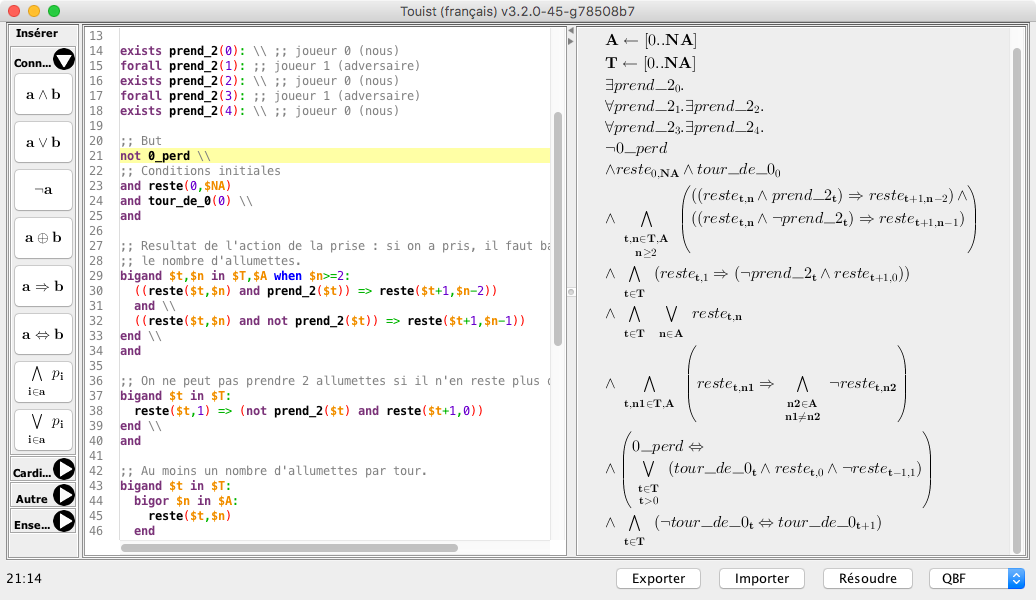
\includegraphics[width=0.9\textwidth]{Pictures/touistScreenshot}
\caption{Capture d'écran de \touist avec le \game. Le fichier est disponible à l'adresse \url{https://github.com/maelvalais/allumettes}}
\label{fig:touistScreenshot}
\end{figure*}

Il faut maintenant définir quand un joueur a perdu :
\begin{gather}
\begin{split}
\lost \lequiv \bigvee_{\substack{t \in \turnsSet\\ t > 0}} & \bigg ( \turn{t} \land \rest{t}{0} %\land \\
%    &  \Big ( \rest{t-1}{1} \lor \rest{t-1}{2} \Big 
\bigg )
\end{split}
\end{gather}
signifie que le joueur $0$ a perdu ssi il existe un tour $t$ où il reste $0$ allumettes alors qu'à l'instant d'avant il y en avait au moins une.

Finalement, à chaque tour $t$, ce n'est pas au joueur $0$ de jouer ssi c'est à lui de jouer au tour suivant :
\begin{gather}
\bigwedge_{t \in \turnsSet \setminus \{ \nbAllumettes \} } \Big (
    \neg \turn{t} \lequiv \turn{t+1}
\Big )
\label{eq:turnChange}
\end{gather}


\subsection{Formalisation d'une stratégie gagnante à l'aide de QBF}
Dans cette section, nous allons présenter à l'aide de notre exemple du \game l'extension de \touist à QBF.

Le langage de QBF permet d'exprimer naturellement et de manière concise l'existence de stratégies gagnantes ainsi que décrit dans \cite{DBLP:series/txtcs/KroeningS16}. Les coups du joueur 0 (pour lequel on cherche une stratégie gagnante) seront existentiellement quantifiés alors que ceux de son adversaire seront universellement quantifiés. (On cherche les coups du joueur $0$ qui le mèneront à la victoire quels que soient les coups joués par le joueur $1$.)

\touist a été étendu pour être compatible avec le solveur QBF \emph{Quantor 3.2} \cite{Biere:2004:RE:2103144.2103150}. La sélection de ce prouveur dans \touist autorise \emph{de facto} l'utilisation des quantificateurs $\forall$ et $\exists$ (respectivement définis par \verb+exists+ et \verb+forall+ dans \touist).

\begin{figure}
\centering
\tikzset{%
    prend1/.style={->,dotted,very thick,>=latex},
    prend2/.style={->,very thick,>=latex}%
}

\begin{tikzpicture}
% définition des noeuds
\node (t0) at (0.5,0) {4};
\node (t11) at (-1,-1) {2};
\node (t12) at (2,-1) {3};
\node (t21) at (-2,-2) {0};
\node (t22) at (0,-2) {1};
\node (t23) at (1,-2) {1};
\node (t24) at (3,-2) {2};
\node (t31) at (0,-3) {0};
\node (t32) at (1,-3) {0};
\node (t33) at (2,-3) {0};
\node (t34) at (4,-3) {1};
\node (t4) at (4,-4) {0};
% 0 joue
\draw[prend2] (t0)--(t11);
\draw[color=red][prend1] (t0)--(t12);
% 1 joue
\draw[prend2] (t11)--(t21);
\draw[prend1] (t11)--(t22);
\draw[color=red][prend2] (t12)--(t23);
\draw[color=red][prend1] (t12)--(t24);
% 0 joue
\draw[prend1] (t22)--(t31);
\draw[color=red][prend1] (t23)--(t32);
\draw[color=red][prend2] (t24)--(t33);
\draw[prend1] (t24)--(t34);
% 1 joue
\draw[prend1] (t34)--(t4);
\end{tikzpicture}

\caption{Solutions pour le \game (4 all./2 joueurs), en rouge : stratégie gagnante du joueur 0}
\label{fig:solutions}
\vspace{-0.5cm}\end{figure}

\tikzset{%
    prend1/.style={->,dotted,very thick,>=latex},
    prend2/.style={->,very thick,>=latex}%
}


\figurename~\ref{fig:solutions} présente l'ensemble exhaustif des solutions de notre exemple. La racine de l'arbre représente le nombre initial d'allumettes, et chaque flèche l'action de retirer $1$ (\tikz{\draw[prend1] (0,0) -- (1,0)}) ou $2$ (\tikz{\draw[prend2] (0,0) -- (1,0)}) allumette(s). Au bout de la flèche, le nombre d'allumettes après exécution de l'action concernée. D'après cette figure, on voit que si le joueur $0$ commence (ce qui est imposé par (\ref{eq:initialState})) et qu'il retire une seule allumette (il en reste donc 3) on voit qu'il a une stratégie gagnante : 
\begin{itemize}
\item si le joueur $1$ retire ensuite $2$ allumettes il en restera $1$ seule que le joueur $0$ peut retirer pour gagner (puisque le joueur $1$ ne pourra ensuite plus retirer d'allumette) ;

\item si le joueur $1$ retire une seule allumette, il en restera  $2$ et le joueur $0$ pourra au coup suivant les retirer en un seul coup et le joueur $1$ perd.
\end{itemize}

Nous tirons parti de QBF pour écrire cette stratégie dans \touist. Si on note $\Phi$ la conjonction des formules (\ref{eq:initialState}) à (\ref{eq:turnChange}) alors la recherche d'une stratégie gagnante pour le joueur $0$ s'écrit simplement :
\vspace{-0.2cm}
\begin{align}
\begin{split}
&\exists \takes{0}
\forall \takes{1}\\
&\qquad\exists \takes{2}
\forall \takes{3} \\
&\quad\exists \takes{4}\text{ . }\neg \lost \land \Phi
\end{split}
\end{align}

\noindent
Autrement dit, on cherche à satisfaire le fait qu'il existe une action du joueur $0$ au tour $0$ telle que quelle que soit l'action du joueur $1$ au tour $1$, il existe une action du joueur $0$ au tour $2$, telle que pour toute action du joueur $1$ au tour $3$ il existe une action du joueur $0$ (qui sera donc le dernier à jouer) telle que le joueur $0$ ne perd pas et que les contraintes inhérentes au \game soient satisfaites.

% \warning{[DOMI : ] Je ne suis pas sûr de ce qui suit car je n'arrive pas à faire fonctionner le prog des allumettes avec la dernière version de \touist (ça plante).}

L'exécution du programme dans \touist indique que cette formule est vraie, ce qui signifie l'existence d'une stratégie gagnante pour le joueur $0$. Le solveur retourne la valeur des (ici une seule) variables existentielles correspondant au prochain coup du joueur $0$. À ce stade, le joueur adverse doit fournir son coup qui fixe la valeur des variables universelles correspondant à ses possibles prochains coups. On exécute alors de nouveau le programme modifié de la façon suivante (de manière à prendre en compte le calcul de la valuation de $\takes{0}$) :
\begin{align*}
\begin{split}
&\exists \takes{0}
\exists \takes{1}\\
&\qquad\exists \takes{2}
\forall \takes{3} \\
&\quad\exists \takes{4}\text{ . }\neg \lost \land c_0 \land c_1 \land  \Phi
\end{split}
\end{align*}
où $c_0$ est soit $\takes{0}$ soit $\neg \takes{0}$ en fonction du coup du joueur $0$, et similairement pour $c_1$ en fonction du coup choisi par l'adversaire. La  situation après ces deux coups est la nouvelle situation initiale pour le solveur et la recherche du coup suivant du joueur $0$... jusqu'à sa victoire ! On réitère ce processus jusqu'à ce que toutes les variables aient reçu une valeur. 
%On obtient alors :
%\begin{gather*}
%\interpret[\takes{0}] = 0, 
%\interpret[\takes{1}] = 1 
%\interpret[\takes{2}] = 0
%\end{gather*}
%qui se lit : pour que le joueur $0$ gagne il doit prendre $1$ allumette, le joueur $1$ en prend $2$, puis le joueur $0$ en prend $1$.

%\section{Codages SAT}
%\subsection{Un exemple de codage : le jeu de Nim}

%\chapter{Planification par satisfaction de formules logiques}
%\section{Planification par compilation}
\section{Planification classique par satisfaction de formules logiques}
%



%%%%%%%%%%%%%%%%%%%%%%%%%%%%%%%%%%%%%%%%%%%%%%%%%%%%%%%
%%%%%%%%%%%%%%%%%%%%%%%%%%%%%%%%%%%%%%%%%%%%%%%%%%%%%%%
%\subsection{Classical STRIPS Planning}
\subsection{Définitions préliminaires}
%%%%%%%%%%%%%%%%%%%%%%%%%%%%%%%%%%%%%%%%%%%%%%%%%%%%%%%
%%%%%%%%%%%%%%%%%%%%%%%%%%%%%%%%%%%%%%%%%%%%%%%%%%%%%%%

%In SAT planning, each copy of the variable set $X$ is indexed, making the writing of transitions easy; let $P$ and $Q$ two formulas and $x_i$ and $x_{i+1}$ two copies of one variable

\begin{definition}
Un \emph{problème de planification classique} STRIPS est un triplet $\langle \F, \I, \A , \G \rangle$ où $\F$ est un ensemble fini de \emph{fluents} (propositions atomiques), $\I \subseteq \F$ est l'ensemble initial de fluents, $\G \subseteq \F$ est l'ensemble des fluents buts et $\A$ est l'ensemble des actions.
Une action $\a \in \A$ est un triplet $\langle \Cond{\a}, \Add{\a}, \Del{\a} \rangle$ où

\begin{itemize}
\item $\Cond{\a} \subseteq \F$ est l'ensemble des fluents requis pour exécuter $\a$ (%les 
\emph{préconditions} de $\a$),
\item $\Add{\a} \subseteq \F$ et $\Del{\a} \subseteq \F$ sont les ensembles de fluents respectivement ajoutés et supprimés par l'action $\a$ (%les 
\emph{ajouts} et %les 
\emph{retraits} de $\a$).
\end{itemize}
\end{definition}


\fred{Ensemble des variables d'actions $X_{\A}$}


\fred{A revoir:}
Nous allons montrer que pour l'approche QBF, au-delà des améliorations sur les solveurs, d'autres travaux doivent être menés pour mettre au point des codages plus performants. Comme nous l'avons indiqué plus haut, cela a été réalisé pour SAT avec des améliorations significatives. Nous présentons ici deux nouveaux codages d'arbres compacts CTE (Compact Tree Encoding) de problèmes de planification en QBF: CTE-EFA basé sur des frame-axiomes explicatifs dans un espace d'états, et CTE-OPEN basé sur des liens de causalité dans un espace de plans. \fred{dans le chapitre EXPERIMENTATIONS:} Nous les comparons au codage de l'état de l'art CTE-NOOP basé sur des actions No-op et proposé dans \cite{DBLP:conf/ecai/CashmoreFG12}. En termes de temps d'exécution par rapport aux problèmes de référence, CTE-EFA et CTE-OPEN sont toujours plus efficaces que CTE-NOOP.


%\begin{itemize}
%\item QBFEVAL’16: largest number of participants ever.
%\item QBF proof systems: theoretical frameworks of solving techniques.
%\item CDCL (clause learning) and expansion: orthogonal solving approaches.
%\item QBF solving by counterexample guided abstraction refinement (CEGAR) [CGJ+03, JM15b, JKMSC16, RT15].
%\item New approaches, e.g., Skolem function computation [RS16].
%\item 10 QBF-related papers at SAT 2016 conference (27\%).
%\end{itemize}

%The QBF approach seems to have several advantages: for comparable SAT / QBF encodings, the size of the generated formulas is more compact \cite{DBLP:conf/ecai/CashmoreFG12}, 

%QBF is a young field of research \cite{DBLP:conf/aaai/CadoliGS98} compared to SAT 
%\begin{itemize}
%\item progrès actuels des solveurs QBF (Qell 10 fois plus rapide sur planning-CTE (qu'est ce que ça veut dire ?) que rareqs, rareqs qui est 2 fois plus rapide que depqbf, chercher refs)
%\item ordre de performance des codages SAT (NOOP+GP, EFA, OPEN) et QBF (EFA, OPEN, NOOP) diffère
%\end{itemize}


%{\color{blue}
%At the time being the SAT approach is actually the best as SAT solvers and encodings have been greatly improved since 1992. So, it would be useless to compare QBF solvers to SAT solvers: the result of the contest is known in advance \cite{DBLP:phd/ethos/Cashmore13}. We believe that, nevertheless, QBF approach to automated planning deserves the interest of the community before it proves to be faster than SAT approach. Our paper shows that beyond the implementation of solvers, further work has to be done on the encodings.

%"Since the first complete QBF solver was presented decades after the first complete engine to solve SAT, research in this field remains at its infancy. compared to SAT (1960s), QBF still is a young field of research"
%}









%%%%%%%%%%%%%%%%%%%%%%%%%%%%%%%%%%%%%%%%%%%%%%%%%%%%%%%%%%%%%%%%%%%%%%%%%%%%%%%%
%%%%%%%%%%%%%%%%%%%%%%%%%%%%%
% PLANIFICATION SAT
%%%%%%%%%%%%%%%%%%%%%%%%%%%%%
\subsection{Codages SAT de référence pour la planification classique}
%

%
% codage SAT-EFA
%
%\subsection{Codage SAT de référence dans les espaces d'états}

\fred{Présenter le codage KS92,95 SAT-EFA classique}

\fred{Attention, ici copier/coller ouvrage SAT 2008 Maris, Régnier, Vidal}
{\color{red}

\subsubsection{Codage dans les espaces d'états avec frame-axiomes explicatifs}

\begin{figure}\label{steps:sat}
\begin{footnotesize}
%(a)\\[1em]

\fred{Rajouter la figure que j'ai enlevée ici !!!}
%   \xymatrix@C=0.1pc@R=1pc{
%   \text{S}_{0} (\textit{Init}) \ar@{->}[r] & \fbox{$x_{1}\equiv$ S$_{1}$} \ar@{>}[r]  & \fbox{$x_{2}\equiv$ S$_{2}$} \ar@{>}[r] & \fbox{$x_{3}\equiv$ S$_{3}$} \ar@{>}[r] & \fbox{$x_{4}\equiv$ S$_{4}$}
%   \ar@{>}[r] & \fbox{$x_{5}\equiv$ S$_{5}$} \ar@{>}[r] & \fbox{$x_{6}\equiv$ S$_{6}$} \ar@{>}[r] & \fbox{$x_{7}\equiv$ S$_{7}$} \ar@{>}[r] & \text{S}_{8} (\textit{Goal})
%   }
\end{footnotesize}
\vspace{1em}
\caption{Transitions of an 8-step plan in SAT/SMT encoding}
\end{figure}


Les codages dans les espaces d'états sont basés sur les transitions entre les étapes successives du plan en partant de l'état initial pour arriver au but.
%Le parallélisme y est codé grâce à la notion d'indépendance entre actions simultanées. 
Pour conserver les fluents non affectés par les actions qui doivent être exécutées dans une étape du plan, on va coder la notion de frame-axiome.
Nous décrivons d'abord la technique la plus efficace en termes de compacité et
de temps de résolution \cite{MK99} qui utilise des frame-axiomes explicatifs.
Nous présentons ensuite une variation de ce codage utilisant des actions
particulières appelées no-ops \cite{KMS96}.
Les règles du codage dans les espaces d'états produisent des propositions de la
forme $a(i)$ qui représentent le fait que l'action $a$ est appliquée à un niveau
$i$ du plan ssi $a(i)$ a la valeur de vérité vrai, et des propositions de la
forme $f(i)$ qui représentent le fait que le fluent $f$ est présent au niveau
$i$ ssi $f(i)$ a la valeur de vérité vrai. Le présence de $f$ au niveau $i$
signifie qu'il est présent après l'application successive de toutes les
actions associées à des propositions qui sont vraies, du niveau 1 jusqu'au
niveau $i$. Ce codage comporte cinq règles~:

\begin{enumerate}
\item \codrule{état initial et but~:} les fluents de l'état initial sont vrais au
  niveau $0$, ceux qui n'en font pas partie sont faux au niveau $0$, et les
  fluents du but sont vrais au niveau $k$.
  \codage{\noindent\left[\biget{f \in I} f(0) \right] \land \left[\biget{f \in (F \setminus I)}\neg f(0) \right] \land \left[\biget{f \in B}f(k) \right]}
\item \label{codage:ee2} \codrule{Préconditions et effets des actions~: } si une
  action appartient au plan, alors ses préconditions sont vérifiées et
  ses effets sont produits.\codage{\biget{i \in [1,k]} \biget{a \in A} \left[
      a_i \Rightarrow \left( \biget{f \in \mathrm{Prec}(a)} f(i-1) \right) \land
      \left( \biget{f \in \mathrm{Add}(a)} f(i) \right) \land \left( \biget{f
          \in \mathrm{Del}(a)} \neg f(i) \right) \right]}
\item \label{codage:ee3} \codrule{Frame-axiomes explicatifs de retrait~:} si un
  fluent devient faux entre deux niveaux successifs du plan, alors une action au
  moins qui le retire doit avoir été appliquée. Il faut que le fluent existe à
  un instant donné, il doit donc appartenir à $I$ ou à $F_a$. Il lui faut aussi
  pouvoir être retiré par une action, il doit donc aussi appartenir à $F_d$.
 \codage{\biget{i \in [1,k]} \biget{f \in ((I \cup F_a) \cap F_d)} \left[ f(i-1) \land \neg f(i) \Rightarrow \bigou{a \in A \suchthat f \in \mathrm{Del}(a)} a(i) \right]}
\item \label{codage:ee4} \codrule{Frame-axiomes explicatifs d'ajout~:} si un
  fluent devient vrai entre deux niveaux successifs du plan, alors une action au
  moins qui l'établit doit avoir été appliquée.  Il faut que le fluent puisse ne
  pas exister à un instant donné, donc ne pas appartenir à $I$ ou appartenir à
  $F_d$. Il lui faut aussi pouvoir être ajouté par une action donc appartenir à
  $F_a$.
  \codage{\biget{i \in [1,k]} \biget{f \in (((F \setminus I) \cup F_d) \cap F_a)} \left[\neg f(i-1) \land f(i) \Rightarrow \bigou{a \in A | f \in \mathrm{Add}(a)} a(i) \right]}
\item \label{codage:ee5} \codrule{Interférences~:} deux actions non
  indépendantes ne peuvent pas être exécutées au même niveau. Les effets
  contradictoires sont déjà pris en compte par la règle \ref{codage:ee2}~; il
  suffit donc d'interdire à un même niveau les actions uniquement interférentes.
  \codage{\biget{i \in [1,k]} \biget{\{a_m, a_n\} \subseteq A \suchthat m < n \land (a_m\|_e a_n) \land \lnot (a_m\|_i a_n)} \left[ \neg a_m(i) \lor \neg a_n(i) \right]}
\end{enumerate}

}

%
% codage SAT-MK99-ESPACES-DE-PLAN
%
\subsection{Codages SAT de référence dans les espaces de plans}

\fred{Présenter les codages MK99 espaces de plans}

\fred{Attention, ici copier/coller ouvrage SAT 2008 Maris, Régnier, Vidal}
{\color{red}
Ces codages ne traduisent plus seulement les transitions qui s'opèrent entre
niveaux successifs du plan, mais expriment maintenant les relations de causalité
entre les actions qui le constituent. Dans les espaces d'états, l'application
des actions est envisagée séquentiellement~: une action ne peut apparaître à un
niveau du plan que lorsque ses préconditions sont satisfaites au niveau
précédent.  Dans les espaces de plans, une action apparaît à un niveau du plan
parce qu'une action d'un niveau antérieur (pas forcément le niveau précédent)
établit ses préconditions et qu'une action qui suit requiert un de ses effets.
L'existence de différents codages découle de la traduction des différentes
stratégies de recherche utilisées dans les espaces de plans. Ces codages restent
moins performants, en termes de compacité et de temps de résolution, que le
meilleur codage dans les espaces d'états (celui avec frame-axiomes explicatifs)
\cite{MK99}.

Dans tous ces codages, les ensembles d'actions indépendants qui peuvent faire
partie d'un plan sont associés à des symboles d'étapes. Un ordre sur ces étapes
détermine un ordre total pour l'exécution des ensembles d'actions indépendants.
Deux étapes particulières sont créées~: l'étape $p_0$ qui représente l'état
initial du problème, et l'étape $p_{k+1}$ qui représente le but du problème. Ces
deux étapes ne contiendront aucune action. Elles sont équivalentes aux actions
fictives $Start$ et $End$ qui servent à initialiser un plan partiel et sont généralement
utilisées en planification dans les espaces de plans partiels. Pour prendre en
compte ces deux étapes, l'ensemble $F_a$ des fluents présents dans les ajouts
des actions est augmenté des fluents de l'état initial $I$. De même, l'ensemble
$F_p$ des fluents présents dans les préconditions des actions est augmenté des
fluents du but $B$. On peut produire des codages produisant moins de clauses en
considérant les actions $Start$ et $End$ comme des cas particuliers
\cite{Vid01}, mais pour des raisons de compacité dans l'écriture des codages
nous les présentons ici de manière intégrée aux autres actions.

Les règles des codages dans les espaces de plans produisent les propositions
suivantes, pour une action $a$, un fluent $f$, et deux étapes $p$ et $q$~:

\begin{itemize}
\item $(a \in p)$ est vraie ssi l'action $a$ appartient à l'étape $p$.
\item $\mathrm{Adds}(p, f)$, est vraie ssi l'étape $p$ contient une action qui ajoute le
  fluent $f$.
\item $\mathrm{Needs}(p, f)$ est vraie ssi l'étape $p$ contient une action qui a $f$ en
  précondition.
\item $\mathrm{Dels}(p, f)$ est vraie ssi l'étape $p$ contient une action qui retire le
  fluent $f$.
\item $p \causal{f} q$ représente un lien causal et est vraie ssi l'étape
  $p$ produit le fluent $f$ qui est une précondition de l'étape $q$.
\item $p \prec q$ est vraie ssi l'étape $p$ précède l'étape $q$~; toutes les actions
  associées à $p$ doivent donc être exécutées avant celles associées à $q$.
  Ces propositions traduisent un ordre partiel sur les étapes.
\end{itemize}


\subsubsection{Partie commune des codages dans les espaces de plans}

Elle permet d'établir une correspondance entre toutes les actions disponibles et
celles qui font partie des étapes des plans solutions. Elle est constituée
de cinq règles~:

\begin{enumerate}
\item \codrule{état initial et but~: } l'étape $p_0$ produit l'état
  initial du problème, et l'étape $p_{k+1}$ requiert les buts.
  \codage{\left[ \biget{f \in I}\mathrm{Adds}(p_0,f)\right] \land \left[ \biget{f \in (F\setminus I)}\lnot\mathrm{Adds}(p_0,f)\right] \land \left[ \biget{f \in B} \mathrm{Needs}(p_{k+1},f)\right]\label{codage:epcom1}}
\item \codrule{Correspondance action/étape~:} si une étape ajoute, retire, ou a
  pour précondition un fluent, alors cette étape peut correspondre à n'importe
  quelle action qui a le même comportement vis-à-vis de ce fluent. Inversement,
  si une action appartient à une étape, ses préconditions, ajouts et retraits
  sont vrais.

  \codage{\biget{i \in [1,k]} \biget{f \in F_a} \left[ \mathrm{Adds}(p_i,f) \Leftrightarrow \bigou{a \in A | f \in \mathrm{Add}(a)} (a \in p_i) \right]\label{codage:epcom2}}
  \codage{\biget{i \in [1,k]} \biget{f \in F_d} \left[ \mathrm{Dels}(p_i,f) \Leftrightarrow \bigou{a \in A | f \in \mathrm{Del}(a)} (a \in p_i) \right]\label{codage:epcom3}}
  \codage{\biget{i \in [1,k]} \biget{f \in F_p} \left[ \mathrm{Needs}(p_i,f) \Leftrightarrow \bigou{a \in A | f \in \mathrm{Prec}(a)} (a \in p_i) \right]\label{codage:epcom4}}
\item \codrule{Exclusions mutuelles~: } deux actions qui ne sont pas indépendantes ne peuvent appartenir à une même étape.
  \codage{\biget{i \in [1,k]} \biget{ \{a_m, a_n\} \subseteq A \suchthat m < n \land \lnot(a_m\|a_n)} \left[\neg (a_m \in p_i) \lor \neg(a_n \in p_i) \right]\label{codage:epcom5}}
\end{enumerate}

\subsubsection{Codage par liens causaux, protection d'intervalles et ordre partiel}

La production des préconditions se fait par le codage direct des liens causaux.
La proposition $p \causal{f} q$ traduit le fait que l'étape $p$ produit le fluent
$f$, précondition de l'étape $q$. La protection de $f$ dans l'intervalle compris
entre les deux étapes se fait par promotion (l'étape menaçant $f$ est placée
avant $p$), ou par rétrogradation (l'étape menaçant $f$ est placée après $q$).
L'ordre d'exécution des étapes  est donné par une relation de précédence de
la forme $p \prec q$. Les quatre règles suivantes sont ajoutées à la partie commune~:

\begin{enumerate}
\item \codrule{Production des préconditions~:} chaque fluent est supporté par un lien
  causal entre l'étape qui le produit et l'étape
  qui l'utilise en tant que précondition.
  \codage{\biget{i \in [1,k+1]} \biget{f\in F_p} \left[ \mathrm{Needs}(p_i, f) \Rightarrow \ifthen{f \in F_a}{\bigou{j \in [0, k] \suchthat j \neq i} p_j \causal{f} p_i}{\bot} \right]}
\item \codrule{Liens causaux~:} un lien causal supportant un fluent $f$ entre
  deux étapes $p_i$ et $p_j$ implique que $p_i$ ajoute $f$, que $p_j$ a pour
  précondition $f$, et que $p_i$ précède $p_j$.
  \codage{\biget{i \in [0,k]} \biget{j \in [1,k+1]\suchthat i\neq j} \biget{f\in (F_p \cap F_a)} \left[ p_i \causal{f} p_j \Rightarrow\left( \mathrm{Adds}(p_i, f) \land \mathrm{Needs}(p_j,f)\land p_i \prec p_j  \right) \right]}
\item \codrule{Protection d'intervalles~:} si un lien causal supporte le
  fluent $f$ entre une étape $p_i$ et une étape $p_j$, et si une étape $p_q$
  retire $f$, alors $p_q$ doit précéder $p_i$ (promotion) ou $p_j$ doit précéder
  $p_q$ (rétrogradation).
  \codage{\biget{i \in [0,k]} \biget{j \in [1,k+1]\suchthat i\neq j} \biget{q \in [1,k]\suchthat q\neq i \land q\neq j} \biget{f\in (F_p \cap F_a \cap F_d)} 
  \left[ \begin{array}{l}p_i \causal{f} p_j \land \mathrm{Dels}(p_q, f) \Rightarrow\\ \left( p_q \prec p_i \lor p_j \prec p_q \right) \end{array} \right]}
\item \codrule{Propriétés de la relation de précédence~:} transitive et
  antisymétrique. L'irréflexivité est codée dans les autres règles par le biais
  des indices des étapes.
  \codage{\biget{i \in [0,k+1]} \biget{j \in [0,k+1]\suchthat i\neq j} \biget{q \in [0,k+1]\suchthat q\neq i \land q\neq j} \left( \left( p_i \prec p_j \land p_j \prec p_q \right) \Rightarrow p_i \prec p_q \right)}
  \codage{\biget{i \in [0,k]} \biget{j \in [i+1,k+1]\suchthat i\neq j} \lnot \left( p_i \prec p_j \right) \lor \lnot \left( p_j \prec p_i \right)}
\end{enumerate}

\subsubsection{Codage par liens causaux, protection d'intervalles et étapes contiguës}

Ce codage simplifie le précédent dans lequel plusieurs modèles correspondent au
même plan solution, à la numérotation des étapes près. Les étapes doivent
maintenant suivre un ordre prédéfini d'indice croissant, ce qui rend inutile la
relation de précédence. La protection d'intervalles ne nécessite plus la
promotion ou la rétrogradation avec un ordre partiel sur les étapes, mais se
réalise en interdisant qu'une étape comprise dans un intervalle défini par un
lien causal ne le menace. Les deux règles suivantes sont ajoutées à la partie
commune~:

\begin{enumerate}
\item \codrule{Production des préconditions~:} chaque fluent est supporté par un
  lien causal entre l'étape qui le produit et l'étape qui l'utilise en tant que
  précondition.
  \codage{\biget{i \in [1,k]} \biget{f\in F_p} \left[ \mathrm{Needs}(p_i, f) \Rightarrow \ifthen{f \in F_a}{\bigou{j \in [1, i-1]} p_j \causal{f} p_i}{\bot}\right]}
\item \codrule{Liens causaux et protection d'intervalles~:} la présence d'un lien
  causal supportant un fluent $f$ entre deux étapes $p_i$ et $p_j$
  implique que $p_i$ ajoute $f$ et que $p_j$ a pour précondition
  $f$. De plus, une étape qui retire $f$ ne peut s'insérer entre $p_i$ et
  $p_j$.
  \codage{\biget{i \in [1,k-1]} \biget{j \in [i+1,k]} \biget{f\in (F_p \cap F_a)} \left[ \begin{array}{l} p_i \causal{f} p_j \Rightarrow \mathrm{Adds}(p_i, f) \land \mathrm{Needs}(p_j,f) \land \\ \ifthen{f \in F_d}{\biget{q\in [i+1,j-1]} \lnot \mathrm{Dels}(p_q, f)}{\top} \end{array}\right]}
\end{enumerate}

\subsubsection{Codage du \enquote{chevalier blanc}}

Ce codage est actuellement le plus compact des codages dans les espaces de plans
en nombre de variables et de clauses produites~; il est également le plus
performant par son temps de résolution. Il exprime directement les liens
causaux~: si une étape requiert un fluent, c'est qu'une étape précédente doit
l'avoir créé. On n'utilise ainsi que les variables déjà présentes dans la partie
commune. La protection d'intervalles se réalise en codant la technique du
\enquote{chevalier blanc} introduite par le planificateur \textsc{Tweak}
\cite{Cha87}. Les deux règles suivantes sont ajoutées à la partie commune~:


\begin{enumerate}
\item \codrule{Production des préconditions~:} la précondition d'une étape d'un niveau
  $i$ doit être ajoutée par une étape précédente.
  \codage{\biget{i \in [1,k+1]} \biget{f\in F_p} \left[ \mathrm{Needs}(p_i, f) \Rightarrow \ifthen{f \in F_a}{\bigou{j \in [0, i-1]} \mathrm{Adds}(p_j, f)}{\bot} \right]}

\item \codrule{Chevalier blanc~:} si une étape a pour précondition le fluent $f$
  au niveau $i$, et qu'une autre le retire au niveau $j$ avant que la première
  puisse l'utiliser, alors il doit y avoir une troisième étape qui rétablit $f$
  à un niveau $q$ tel que $j < q < i$.
  \codage{\biget{i \in [3,k+1]} \biget{j \in [1,i-2]} \biget{f \in (F_p \cap F_d)} \left[ \begin{array}{l}\mathrm{Needs}(p_i, f) \land \mathrm{Dels}(p_j, f) \Rightarrow\\ 
        \ifthen{f \in F_a}{\bigou{q \in [j+1,i-1]} \mathrm{Adds}(p_q,f)}{\bot}\end{array} \right]}
\end{enumerate}


}

%
% codage SAT-OPEN
%
\subsection{Nouveau codage SAT dans les espaces de plans}

\fred{A ajouter: complexité en espace meilleure par rapport à MK99}

Les codages SAT dans les espaces de plans existants introduits par \cite{DBLP:conf/aaai/MaliK99} se r\'{e}f\`{e}rent tous \`{a} trois \'{e}tapes index\'{e}es (pas n\'{e}cessairement cons\'{e}cutives) du plan.
Dans notre nouveau codage, nous allons nous r\'{e}f\'{e}rer seulement \`{a} deux \'{e}tapes cons\'{e}cutives.
Pour chaque action $\a\in\A$ et chaque \'{e}tape $i$, nous cr\'{e}ons une variable propositionnelle $\a_{i}$ pour d\'{e}terminer qu'une instance de $\a$ doit \^{e}tre planifi\'{e}e \`{a} l'\'{e}tape $i$.
Pour chaque fluent $\f\in\F$ et chaque \'{e}tape $i$, nous cr\'{e}ons une variable propositionnelle $\open{\f}{i}$ pour exprimer que $\f$ se maintient \`{a} l'\'{e}tape pr\'{e}c\'{e}dente $i-1$ et doit \^{e}tre prot\'{e}g\'{e} au moins jusqu'\`{a} l'\'{e}tape $i$.

\begin{figure}[hb!]\centering
	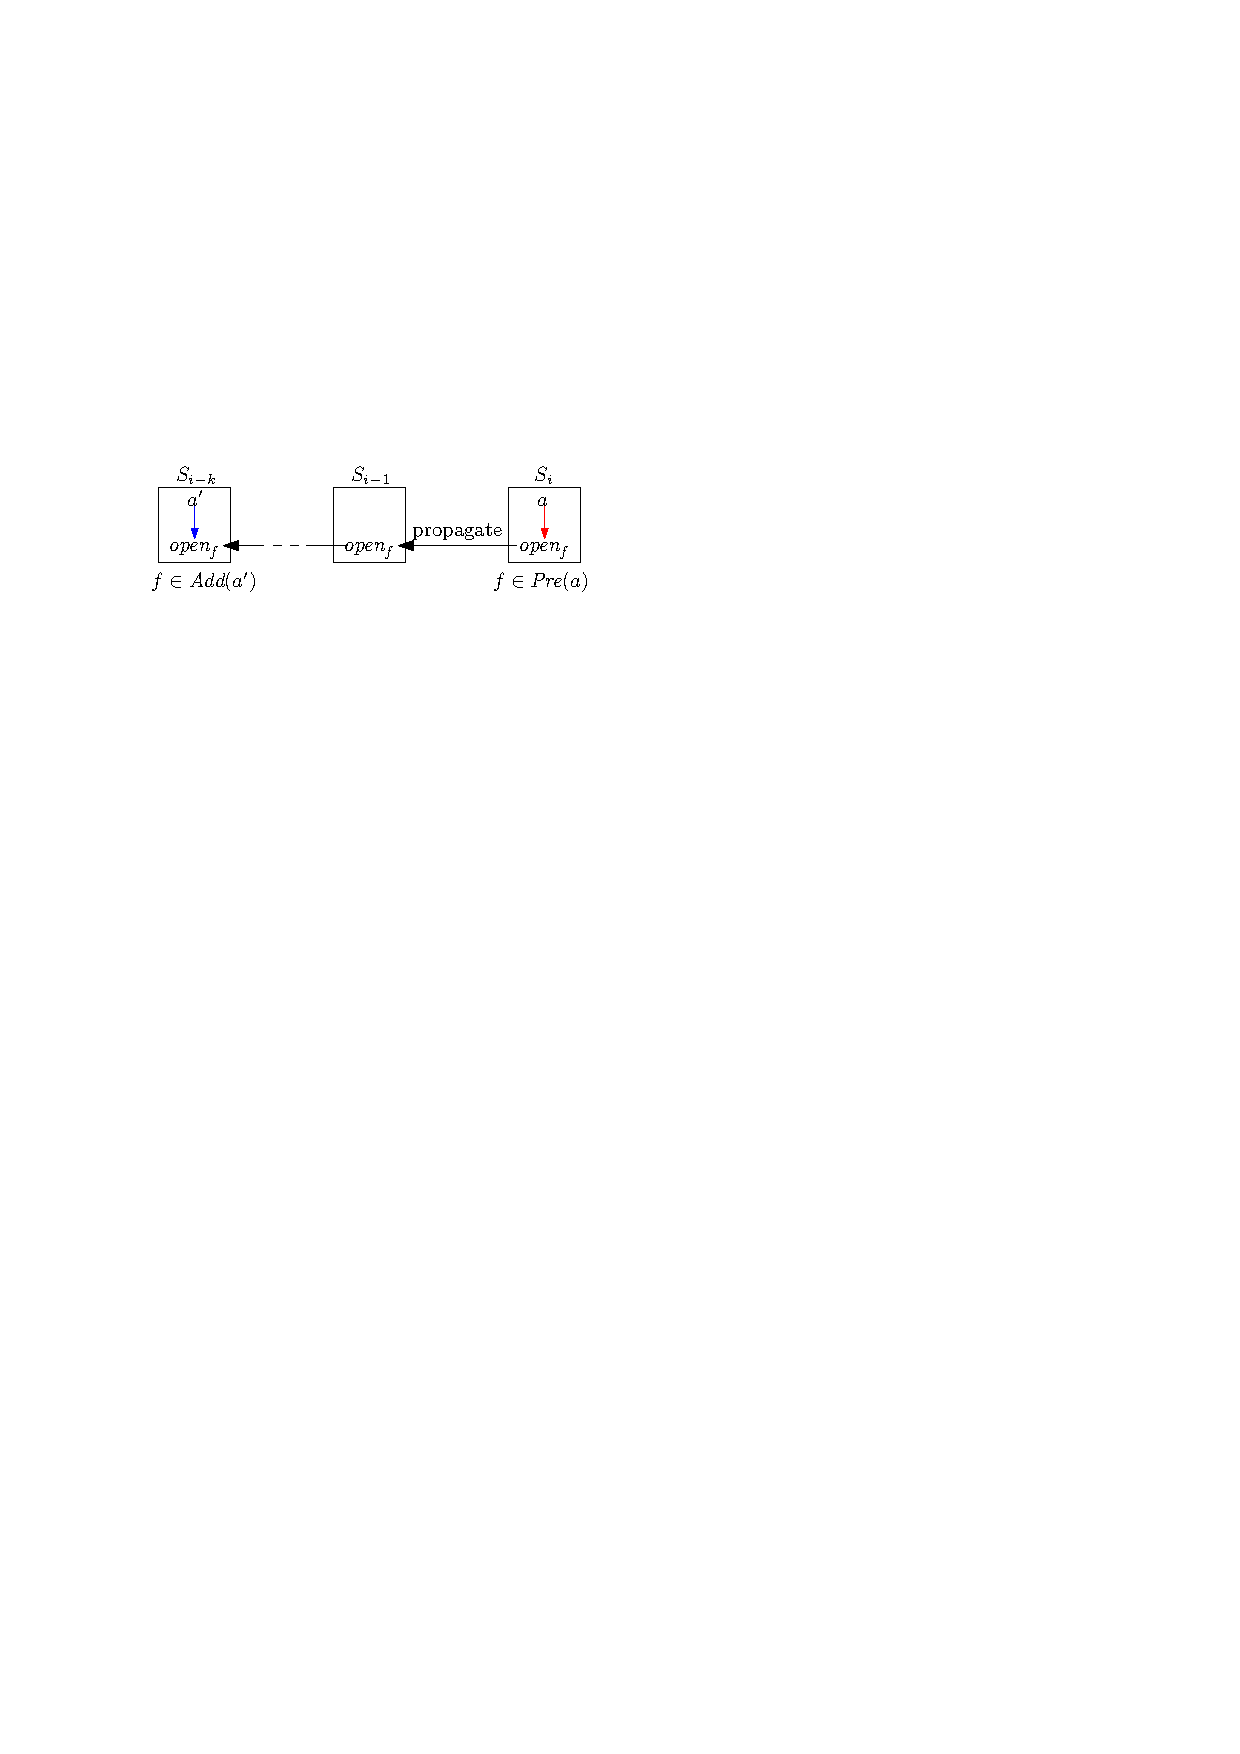
\includegraphics[width=.4\textwidth]{figures/transitions}
    \caption{Lien causal: l'action $a'$ produit $\f$ \`{a} l'\'{e}tape $S_{i-k}$ pour l'action $\a$ qui n\'{e}cessite $\f$ \`{a} l'\'{e}tape $S_{i}$.}
    \label{fig:causal-link}
\end{figure}

Dans la figure~\ref{fig:causal-link}, la variable $f$ est une \textit {condition ouverte} \`{a} l'\'{e}tape $\S_i$, impliquant que $\f\in\I$ ou une action $a'$ qui ajoute $\f$ est ex\'{e}cut\'{e}e dans une \'{e}tape pr\'{e}c\'{e}dente $\S_{i-k}$.
Les conditions ouvertes doivent \^{e}tre propag\'{e}es vers l'arri\`{e}re jusqu'\`{a} l'\'{e}tat initial ou une \'{e}tape dans laquelle elles sont ajout\'{e}es par une action.




%\paragraph*{SAT Encodings for Classical Planning}
%%\begin{figure}\label{steps:sat}
%%\begin{tiny}
%%%(a)\\[1em]
%%  \xymatrix@C=0.1pc@R=1pc{
%%  \text{S}_{0} (\textit{Init}) \ar@{>}[r] & \fbox{$x_{1}\equiv$ S$_{1}$} \ar@{>}[r]  & \fbox{$x_{2}\equiv$ S$_{2}$} \ar@{>}[r] & \fbox{$x_{3}\equiv$ S$_{3}$} \ar@{>}[r] & \fbox{$x_{4}\equiv$ S$_{4}$}
%%  \ar@{>}[r] & \fbox{$x_{5}\equiv$ S$_{5}$} \ar@{>}[r] & \fbox{$x_{6}\equiv$ S$_{6}$} \ar@{>}[r] & \fbox{$x_{7}\equiv$ S$_{7}$} \ar@{>}[r] & \text{S}_{8} (\textit{Goal}) \\
%%  }
%%\end{tiny}
%%%(b)\\[1em]
%%%   \hspace{0.8em}\xymatrix@C=0pc@R=1pc{
%%%   & & & & & \fbox{$x_{2}\equiv$ S$_{4}$} \ar@{.}[lld] \ar@{.}[rrd] \ar@/^1pc/[rdd] & & & & \\
%%%   & & & \fbox{$x_{1}\equiv$ S$_{2}$} \ar[rd] & & & & \fbox{$x_{1}\equiv$ S$_{6}$} \ar[rd] & & \\
%%%   \text{S}_{0} (\textit{Init}) \ar@{>}[rr] & & \fbox{$x_{0}\equiv$ S$_{1}$} \ar[ru]  & & \fbox{$x_{0}\equiv$ S$_{3}$} \ar@/^1pc/[ruu] & &  \fbox{$x_{0}\equiv$ S$_{5}$} \ar[ru] & & \fbox{$x_{0}\equiv$ S$_{7}$} \ar@{>}[rr] & & \text{S}_{8} (\textit{Goal}) \\
%%%  }
%%\vspace{1em}
%%\caption{Transitions of an 8-steps plan in SAT/SMT encoding}
%%\end{figure}
%  Each step $i$ is associated with:\hfill
%  \begin{itemize}
%    \item a set of propositional variables for actions $\{a_{i}^{1},a_{i}^{2}\ldots,a_{i}^{m}\}$
%    \item a set of propositional variables for open conditions $\{open_{f^1,i},open_{f^2,i},\ldots,open_{f^n,i}\}$ %which determine their value in state $x_{i-1}$
%  \end{itemize}


%\begin{frame}{SAT Encoding: open conditions}
%Given a propositional formula $\varphi$, $\textit{open}_{\varphi} = \textit{NNF}_{\textit{open}}(+1,\varphi)$ with:\\[0.8em]
%\begin{itemize}
%  \item $\textit{NNF}_{\textit{open}}(+1,f) = \textit{open}_{f}$
%  \item $\textit{NNF}_{\textit{open}}(-1,f) = \textit{open}_{\neg f}$\\[0.8em]
%  \item $\textit{NNF}_{\textit{open}}(+1,\neg \varphi) = \textit{NNF}_{\textit{open}}(-1,\varphi)$
%  \item $\textit{NNF}_{\textit{open}}(-1,\neg \varphi) = \textit{NNF}_{\textit{open}}(+1,\varphi)$\\[0.8em]
%  \item $\textit{NNF}_{\textit{open}}(+1,\varphi_{1} \wedge \varphi_{2}) = \textit{NNF}_{\textit{open}}(+1,\varphi_{1}) \wedge \textit{NNF}_{\textit{open}}(+1,\varphi_{2})$
%  \item $\textit{NNF}_{\textit{open}}(-1,\varphi_{1} \wedge \varphi_{2}) = \textit{NNF}_{\textit{open}}(-1,\varphi_{1}) \vee \textit{NNF}_{\textit{open}}(-1,\varphi_{2})$\\[0.8em]
%   \item $\textit{NNF}_{\textit{open}}(+1,\varphi_{1} \vee \varphi_{2}) = \textit{NNF}_{\textit{open}}(+1,\varphi_{1}) \vee \textit{NNF}_{\textit{open}}(+1,\varphi_{2})$
%   \item $\textit{NNF}_{\textit{open}}(-1,\varphi_{1} \vee \varphi_{2}) = \textit{NNF}_{\textit{open}}(-1,\varphi_{1}) \wedge \textit{NNF}_{\textit{open}}(-1,\varphi_{2})$\\[0.8em]
%\end{itemize}
%\end{frame}


%\paragraph*{SAT Encoding: open conditions, then propagate or close}

Dans la suite, nous donnons notre codage pour une longueur de plan fix\'{e}e $\length$. Une borne sup\'{e}rieure pour $\length$ est le nombre total d'\'{e}tats possibles, soit $2^{\mid\F\mid}$.

\paragraph*{Conditions ouvertes}

Si une action $\a$ est ex\'{e}cut\'{e}e dans une \'{e}tape du plan, alors chaque condition de $\a$ doit \^{e}tre une condition ouverte \`{a} cette \'{e}tape (c'est-\`{a}-dire qu'un lien causal est requis pour cette condition).


\begin{small}
\begin{multline*}
~\\[-3em]
\bigwedge\limits_{\substack{\mathbf{i}\in [1..\mathbf{\length}]}}\bigwedge\limits_{\substack{\mathbf{\a}\in \mathbf{\A}}}\left(\mathbf{\a}_{\mathbf{i}} \Rightarrow \bigwedge\limits_{\substack{\mathbf{\f}\in \pre{\mathbf{\a}}}}open_{\mathbf{\f},\mathbf{i}}\right)\hfill\\[-2em]
%%%
\end{multline*}
\end{small}

Dans la derni\`{e}re \'{e}tape du plan menant au but tous les fluents du but doivent \^{e}tre des conditions ouvertes ou ajout\'{e}es par des actions ex\'{e}cut\'{e}es dans cette \'{e}tape.

\begin{small}
\begin{multline*}
~\\[-3em]
\bigwedge\limits_{\substack{\mathbf{\f}\in \mathbf{\G}}}\left(open_{\mathbf{\f},\mathbf{\length}} \vee \bigvee\limits_{\substack{\mathbf{\a}\in \mathbf{\A}\\\mathbf{\f} \in \add{\mathbf{\a}}}}\mathbf{\a}_{\mathbf{\length}}\right)\hfill\\[-2em]
%%%
\end{multline*}
\end{small}

\paragraph*{Propagation et fermeture}

Aucune condition ne doit rester ouverte dans la premi\`{e}re \'{e}tape du plan si elle n'est pas fournie dans l'\'{e}tat initial.
%$\bigwedge_{\mathbf{\f}\in \mathbf{\F}\setminus \mathbf{I}}\neg open_{\mathbf{\f},1}$

\begin{small}
\begin{multline*}
~\\[-3em]
\bigwedge\limits_{\substack{\mathbf{\f}\in \mathbf{\F}\setminus \mathbf{I}}}\neg open_{\mathbf{\f},1}\hfill\\[-2em]
%%%
\end{multline*}
\end{small}

Toute condition ouverte dans une \'{e}tape doit soit rester ouverte soit \^{e}tre ajout\'{e}e (ferm\'{e}e) par une action \`{a} l'\'{e}tape pr\'{e}c\'{e}dente.

\begin{small}
\begin{multline*}
~\\[-3em]
\bigwedge\limits_{\substack{\mathbf{i}\in [2..\mathbf{\length}]}}\bigwedge\limits_{\substack{\mathbf{f}\in \mathbf{\F}}}\left(open_{\mathbf{\f},\mathbf{i}} \Rightarrow \left(open_{\mathbf{\f},\mathbf{i} - 1} \vee \bigvee\limits_{\substack{\mathbf{\a}\in \mathbf{\A}\\\mathbf{\f} \in \add{\mathbf{\a}}}}\mathbf{\a}_{\mathbf{i} - 1}\right)\right)\hfill\\[-2em]
%%%
\end{multline*}
\end{small}


%\paragraph*{SAT Encoding: protect open conditions and prevent negative interactions (mutex)}

\paragraph*{Protection des conditions ouvertes}

Une condition ouverte dans une \'{e}tape donn\'{e}e ne peut pas \^{e}tre supprim\'{e}e \`{a} l'\'{e}tape pr\'{e}c\'{e}dente. Cela garantit de ne rompre aucun lien de causalit\'{e} dans le plan.
\begin{small}
\begin{multline*}
~\\[-3em]
\bigwedge\limits_{\substack{\mathbf{i}\in [2..\mathbf{\length}]}}\bigwedge\limits_{\substack{\mathbf{\f}\in \mathbf{\F}}}\left(open_{\mathbf{\f},\mathbf{i}} \Rightarrow \bigwedge\limits_{\substack{\mathbf{\a}\in \mathbf{\A}\\\mathbf{\f} \in \del{\mathbf{\a}}}}\neg \mathbf{\a}_{\mathbf{i} - 1}\right)\hfill\\[-3em]
%%%
\end{multline*}
\end{small}

\paragraph*{Pr\'{e}vention des interactions n\'{e}gatives}

Si une action supprime un fluent qui est n\'{e}cessaire ou est ajout\'{e} par une autre action, alors ces deux actions ne peuvent pas \^{e}tre ex\'{e}cut\'{e}es toutes les deux dans une m\^{e}me \'{e}tape.

\begin{small}
\begin{multline*}
~\\[-3em]
\bigwedge\limits_{\substack{\mathbf{i}\in [1..\mathbf{length}]}}\bigwedge\limits_{\substack{\mathbf{\a}\in \mathbf{\A}}}\bigwedge\limits_{\substack{\mathbf{f}\in \left(\add{\mathbf{\a}}\cup\pre{\mathbf{\a}}\right)}}\bigwedge\limits_{\substack{\mathbf{\b}\in \mathbf{\A}\\\mathbf{\a} \neq \mathbf{\b} \wedge \mathbf{f} \in \del{\mathbf{\b}}}}\left(\neg \mathbf{\a}_{\mathbf{i}} \vee \neg \mathbf{\b}_{\mathbf{i}}\right)\hfill\\[-3em]
\end{multline*}
\end{small}


Dans la section suivante, nous présentons une version plus compacte de ce nouveau codage qui utilise le langage QBF. Nous \'{e}tendons ensuite ce codage SAT pour la planification classique en un codage SMT pour la planification temporelle en temps continu.




%%%%%%%%%%%%%%%%%%%%%%%%%%%%%%%%%%%%%%%%%%%%%%%%%%%%%%%%%%%%%%%%%%%%%%%%%%%%%%%%
%%%%%%%%%%%%%%%%%%%%%%%%%%%%%
% PLANIFICATION QBF
%%%%%%%%%%%%%%%%%%%%%%%%%%%%%
\subsection{Codages QBF de référence pour la planification classique}\label{chap:codages:qbf:reference}
%

Deux approches différentes de la planification QBF ont été proposées par \cite{DBLP:conf/ecai/CashmoreFG12}:
Le codage plat ou \textit{Flat Encoding} (FE), qui a été introduit par \cite{DBLP:conf/lpar/Rintanen01} et le codage d'arbre compact ou \textit{Compact Tree Encoding} (CTE)  %\citeauthor{DBLP:conf/ecai/CashmoreFG12} ont montré dans
\cite{DBLP:conf/ecai/CashmoreFG12} %que les codages d'arbres compacts 
qui surpasse le codage plat.
Ces deux codages de planification utilisent la structure de branchement de QBF pour réutiliser un seul ensemble de clauses qui décrit une seule étape dans le plan. Les deux affectations possibles de chaque variable universelle y représentent la première et la seconde moitié du plan réparties autour de cette branche. Les affectations de chaque ensemble existentiel représentent des choix d'action dans une seule étape.

\begin{figure}[h]\label{steps2}
\begin{footnotesize}
(a)\\[1em]
  \xymatrix@C=0.1pc@R=1pc{
  \text{S}_{0} (\textit{Init}) \ar@{>}[r] & \fbox{$x_{1}\equiv$ S$_{1}$} \ar@{>}[r]  & \fbox{$x_{2}\equiv$ S$_{2}$} \ar@{>}[r] & \fbox{$x_{3}\equiv$ S$_{3}$} \ar@{>}[r] & \fbox{$x_{4}\equiv$ S$_{4}$}
  \ar@{>}[r] & \fbox{$x_{5}\equiv$ S$_{5}$} \ar@{>}[r] & \fbox{$x_{6}\equiv$ S$_{6}$} \ar@{>}[r] & \fbox{$x_{7}\equiv$ S$_{7}$} \ar@{>}[r] & \text{S}_{8} (\textit{Goal}) \\
  }
  ~\\[3em]
(b)\\[-1em]
   \hspace{0.8em}\xymatrix@C=0pc@R=1pc{
   & & & & & \fbox{$x_{2}\equiv$ S$_{4}$} \ar@{.}[lld] \ar@{.}[rrd] \ar@/^1pc/[rdd] & & & & \\
   & & & \fbox{$x_{1}\equiv$ S$_{2}$} \ar[rd] & & & & \fbox{$x_{1}^{\prime}\equiv$ S$_{6}$} \ar[rd] & & \\
   \text{S}_{0} (\textit{Init}) \ar@{>}[rr] & & \fbox{$x_{0}\equiv$ S$_{1}$} \ar[ru]  & & \fbox{$x_{0}^{\prime}\equiv$ S$_{3}$} \ar@/^1pc/[ruu] & &  \fbox{$x_{0}^{\prime\prime}\equiv$ S$_{5}$} \ar[ru] & & \fbox{$x_{0}^{\prime\prime\prime}\equiv$ S$_{7}$} \ar@{>}[rr] & & \text{S}_{8} (\textit{Goal}) \\
  }
\vspace{2em}
 \end{footnotesize}
\caption{Transitions pour un plan en 8 étapes : (a) codage SAT/SMT et (b) codage d'arbre compact QBF (CTE)}
\end{figure}


%
% codage QBF-FE (Flat Encoding)
%


\subsubsection{Principe des codages plats QBF}

\fred{Schéma de principe}


%
% codage CTE-NOOP
%


%In their paper, \citeauthor{DBLP:conf/ecai/CashmoreFG12} also give a correctness proof that applies to any CTE encoding implementing any transition function. In the following, we stay in this 


\subsubsection{Codages d'arbres compacts QBF avec actions No-op}


%\noindent A \textit{state} $\S$ is a valuation of the fluent set $\F$.
\begin{figure} \centering\mbox{
 \xymatrix@C=0.6pc@R=1.2pc{ %changer @C=0.55pc pour article en double colonne
    & & & & \X_i \ar@{-}[llld]_{b_i=\bot} \ar@{-}[rrrd]^{b_i=\top} \ar@*{[blue]}@/^1.5pc/[rddddd]_{\color{blue} \rightselect{i}} & \\
    & \X_{i-1} \ar@{.}[ld] \ar@{-}[rd]^{b_{i-1}=\top} & & &  & & & \X_{i-1} \ar@{-}[ld]_{b_{i-1}=\bot} \ar@{.}[rd]\\
    & & \X_{i-2}  \ar@{.}[ld]_{b_{i-2}=\bot} \ar@{.}[rddd]_>>>>>{b_{\{i-2, \ldots, 1\}}=\top} & & & & \X_{i-2} \ar@{.}[lddd]^>>>>>{b_{\{i-2, \ldots, 1\}}=\bot} \ar@{.}[rd]^{b_{i-2}=\top} & &\\
    & & & & & & & & & \\
    & & & & & & & & & \\
    & & & \X_{0} \ar@*{[red]}@/^1.5pc/[ruuuuu]_{\color{red} \leftselect{i}} & & \X_{0} & \\
 } }
\caption{Les deux types de transitions possibles dans un CTE suivant la structure de branchement d'une QBF: $\X_0\rightarrow \X_i$ ({\color{red}d'une feuille vers un n\oe ud à gauche}) et $\X_i\rightarrow \X_0$ ({\color{blue}d'un n\oe ud vers une feuille à droite}). Notons que $i$ fait référence à n'importe quel niveau (excepté pour le niveau feuille), pas seulement la racine.} \label{fig:plantree}
\end{figure}

% \mael{Peut-être ajouter des définition
% \begin{itemize}
% \item A state $\S$ is defined as a subset of $\F$,
% \item A \emph{compound action} $\hat{\a}$ is a set of actions,
% \item A \emph{plan} is a sequence of states $\S_0, \dots, \S_n$ such that 
% \[ \displaystyle \forall_{i = 1}^{n} \S_{i-1} = (\S_i \setminus \cup_{\a \in \hat{\a}} \Del{\a}) \cup_{\a \in \hat{\a} \Add{\a}} \text{and} \S_{i-1}\]
% \item An action $A$ is \emph{applicable} iff from a state $S$
% \end{itemize}

% }

Tous les codages QBF étudiés dans cet article utilisent des variables propositionnelles pour les actions. Le codage d'arbre compact proposé dans \cite{DBLP:conf/ecai/CashmoreFG12} est basé sur le \textit{graphe de planification} introduit dans \cite{BF97} et utilise des actions No-op supplémentaires comme frame-axiomes. Nous nommerons ce codage CTE-NOOP.
Chaque action étant considérée comme une variable propositionnelle, nous définissons un ensemble de variables propositionnelles $\X$, donné par $\X = \A \cup \{\noopSingle{f}\mid \f\in\F\}$.

Dans une formule CTE, il faut pouvoir sélectionner deux étapes consécutives du plan afin de définir des transitions (Figure~\ref{fig:plantree}). Pour chaque profondeur $i$ de l'arbre, $\X_i$ dénote une copie de l'ensemble des variables $\X$.

Pour CTE-NOOP, il existe une seule variable $\a_{i}\in X_{i}$ pour chaque action et une seule variable $\noop{\f}{i}\in X_{i}$ (action No-op) pour chaque fluent utilisée pour déterminer une transition dans le plan. A la même profondeur $i$, la valeur de ces variables dépend du n\oe ud (correspondant à une étape du plan) sélectionné par les valeurs des variables universelles de branchement supérieures $b_{i+1}\ldots b_{\depth}$. Pour plus de détails, on pourra se reporter aux explications données dans les transparents en ligne\footnote{\url{https://www.irit.fr/~Frederic.Maris/documents/coplas2018/slides.pdf}}.

Une limite supérieure à la longueur du plan est $2^{k+1}-1$, où $k$ est le nombre d'alternances de quantificateurs dans la formule booléenne quantifiée associée au problème de planification. Dans le cas d'un CTE, $k$ est aussi la profondeur de l'arbre compact. Le nombre d'états possibles pour un problème de planification donné est limité par $2^{\mid \F \mid}$. Ainsi, l'existence d'un plan peut être déterminée en utilisant un codage QBF linéaire avec au plus $k=\mid \F \mid$.



\paragraph*{Quantificateurs}

%In a CTE formula, we want to select two consecutive steps in order to define transitions (Figure~\ref{fig:plantree}).
Pour chaque profondeur $i$ de l'arbre, $\X_i$ dénote une copie de l'ensemble des variables $\X$. Il existe une seule variable $\a_{i}\in X_{i}$ pour chaque action utilisée pour déterminer la dernière transition dans le plan et une seule variable $\noop{\f}{i}\in X_{i}$ pour chaque action No-op correspondant au maintien du fluent $\f$. A la même profondeur~$i$, la valeur de ces variables dépend du n\oe ud (correspondant à une étape du plan) sélectionné par les valeurs des variables universelles de branchement supérieures $b_{i+1}\ldots b_{\depth}$.

\begin{small}
\[
\begin{matrix}
\displaystyle \bigexists_{\a \in \A} \a_{\depth}. \bigexists_{\f\in \F} \noop{\f}{\depth}.%\\
\displaystyle {\bigforall b_{\depth}.}\\
\displaystyle \bigexists_{\a \in \A} \a_{\depth-1}. \bigexists_{\f\in \F} \noop{\f}{\depth-1}.%\\
\displaystyle {\bigforall b_{\depth-1}.}\\
\displaystyle \dots\\ 
%\dots
\displaystyle \bigexists_{\a \in \A} \a_{1}. \bigexists_{\f\in \F} \noop{\f}{1}.%\\
\displaystyle {\bigforall b_{1}.}%\\
\displaystyle \bigexists_{\a \in \A} \a_{0}. \bigexists_{\f\in \F} \noop{\f}{0}.
\end{matrix}
\]
\end{small}\\

Dans ce qui suit, un \textit{n\oe ud} désigne maintenant un n\oe ud qui n'est pas une feuille. % et $\depth$ est la profondeur de l'arbre.
Le prédécesseur d'un n\oe ud au niveau $i$ est la feuille la plus à droite du sous-arbre gauche. Le successeur d'un noeud au niveau $i$ est la feuille la plus à gauche du sous-arbre droit.
Afin de sélectionner ces transitions, nous introduisons l'opérateur feuille-vers-n\oe ud $\leftselect{i}$ défini comme:
%\begin{scriptsize}
\[\leftselect{i} \equiv \neg b_{i} \wedge \BigforallTwo{j=1}{i-1} b_{j}.\]
%\end{scriptsize}
Symétriquement, nous introduisons l'opérateur n\oe ud-vers-feuille $\rightselect{i}$ défini comme:
%\begin{scriptsize}
\[\rightselect{i} \equiv b_{i} \wedge \BigforallTwo{j=1}{i-1} \neg b_{j}.\]
%\end{scriptsize}


\paragraph*{Première étape du plan}

Une action ne peut pas être exécutée dans la première étape du plan si l'ensemble de ses préconditions ne sont pas présentes dans l'état initial du problème. De même, une action No-op d'un fluent $\f$ ne peut pas être exécutée dans cette première étape si le fluent $\f$ n'est pas dans l'état initial.

\begin{small}
\[
\begin{matrix}
\BigforallTwo{i=1}{\depth} \neg b_{i} \Rightarrow \left( \left(\Bigforall{\substack{\a \in \A\\\neg \left(\Cond{\a}\subseteq \I\right)}} \neg \a_{0} \right)
\wedge \left(\Bigforall{\f\in \left(\F\setminus \I\right)}\neg \noop_{\f,0}\right)\right)\\
\end{matrix}
\]
\end{small}\\

\paragraph*{Dernière étape du plan}

Dans la dernière étape du plan, tous les buts doivent être produits par une action (dans $\A$ ou No-op).

\begin{small}
\[
\begin{matrix}
\BigforallTwo{i=1}{\depth} b_{i} \Rightarrow \Bigforall{\f\in \G}\left(\left(\Bigexists{\substack{\a\in\A\\ \f \in \Add{\a}}} \a_{0}\right) \vee \noop{\f}{0}\right)
\end{matrix}
\]
\end{small}\\

\paragraph*{Préconditions des actions}

Si une action est exécutée dans une étape du plan alors chacune de ses préconditions doit être produite à l'étape précédente par une action (dans $\A$ ou No-op).

\begin{small}
\[
\begin{matrix}
\BigforallTwo{i=1}{\depth} \Bigforall{\a\in\A} \Bigforall{\f\in \Cond{\a}} \left(\left(\a_{i} \wedge \leftselect{i} \right) \Rightarrow \left(\noop{\f}{0} \vee \bigvee\limits_{\substack{\b \in \A \\ \f \in \Add{\b}}} \b_{0}\right)\right)\\
\BigforallTwo{i=1}{\depth} \Bigforall{\a\in\A} \Bigforall{\f\in \Cond{a}}\left(\left(\a_{0} \wedge \rightselect{i} \right) \Rightarrow \left(\noop{\f}{i} \vee \bigvee\limits_{\substack{\b \in \A \\ \f \in \Add{\b}}} \b_{i}\right)\right)
\end{matrix}
\]
\end{small}\\

De même, si une action No-op est exécutée dans une étape du plan alors le fluent correspondant doit être produit à l'étape précédente par une action (dans $\A$ ou No-op).

\begin{small}
\[
\begin{matrix}
\BigforallTwo{i=1}{\depth} \Bigforall{\f\in \F} \left(\left(\noop{\f}{i} \wedge \leftselect{i} \right) \Rightarrow \left(\noop{\f}{0} \vee \bigvee\limits_{\substack{\a \in \A \\ \f \in \Add{\a}}} \a_{0}\right)\right)\\
\BigforallTwo{i=1}{\depth}\Bigforall{\f\in \F}\left(\left(\noop{\f}{0} \wedge \rightselect{i} \right) \Rightarrow \left(\noop{\f}{i} \vee \bigvee\limits_{\substack{\a \in \A \\ \f \in \Add{\a}}} \a_{i}\right)\right)
\end{matrix}
\]
\end{small}\\

\paragraph*{Prévention des interactions négatives}

Si une action supprime un fluent qui est nécessaire ou est ajouté par une autre action, alors ces deux actions ne peuvent pas être exécutées toutes les deux dans une même étape. De même, une action qui détruit un fluent $\f$ ne peut être exécutée à une même étape que l'action No-op de $\f$.
%\begin{scriptsize}
\[ \BigforallTwo{i=0}{\depth} \Bigforall{\a \in \A} \Bigforall{\f\in \left(\Add{\a} \cup \Cond{\a}\right)} \Bigforall{\b \in \A \\ \a \neq \b \\ \f \in \Del{\b}}\left(\neg \a_{i} \vee \neg \b_{i}\right) \]
%\end{scriptsize}

\[ \BigforallTwo{i=0}{\depth} \Bigforall{\a\in \A} \Bigforall{\f \in \Del{\a}}\left(\neg \noop{\f}{i} \vee \neg \a_{i}\right) \]


%\begin{multline*}
%\displaystyle\mathop{\exists \mathbf{A}_{2}}_{\mathbf{A}\in \mathbf{O}} .\displaystyle\mathop{\exists Noop_{\mathbf{f},2}}_{\mathbf{f}\in \mathbf{F}} .\exists b_{2}. \displaystyle\mathop{\exists \mathbf{A}_{1}}_{\mathbf{A}\in \mathbf{O}} .\displaystyle\mathop{\exists Noop_{\mathbf{f},1}}_{\mathbf{f}\in \mathbf{F}} .\exists b_{1}. \displaystyle\mathop{\exists \mathbf{A}_{0}}_{\mathbf{A}\in \mathbf{O}} .\displaystyle\mathop{\exists Noop_{\mathbf{f},0}}_{\mathbf{f}\in \mathbf{F}}.\\
%
%\bigwedge\limits_{\substack{\mathbf{A}\in \mathbf{O}\\\neg \left(\mathbf{Cond}_{\mathbf{A}}\subseteq \mathbf{I}\right)}}\left(\neg \mathbf{A}_{0} \vee \left(\bigvee\limits_{\substack{\mathbf{i}\in [1..\mathbf{depth}]}}b_{\mathbf{i}}\right)\right)\\
%
% \wedge \bigwedge\limits_{\substack{\mathbf{f}\in \left(\mathbf{F}\setminus \mathbf{I}\right)}}\left(\neg Noop_{\mathbf{f},0} \vee \left(\bigvee\limits_{\substack{\mathbf{i}\in [1..\mathbf{depth}]}}b_{\mathbf{i}}\right)\right)\\
%
% \wedge \bigwedge\limits_{\substack{\mathbf{f}\in \mathbf{G}}}\left(\left(\bigvee\limits_{\substack{\mathbf{A}\in \mathbf{O}\\\mathbf{f} \in \mathbf{Add}_{\mathbf{A}}}}\mathbf{A}_{0}\right) \vee Noop_{\mathbf{f},0} \vee \left(\bigvee\limits_{\substack{\mathbf{i}\in [1..\mathbf{depth}]}}\neg b_{\mathbf{i}}\right)\right)\\
%
% \wedge \bigwedge\limits_{\substack{\mathbf{i}\in [1..\mathbf{depth}]}}\bigwedge\limits_{\substack{\mathbf{A}\in \mathbf{O}}}\bigwedge\limits_{\substack{\mathbf{f}\in \mathbf{Cond}_{\mathbf{A}}}}\left(\neg \mathbf{A}_{\mathbf{i}} \vee \left(\bigvee\limits_{\substack{\mathbf{B}\in \mathbf{O}\\\mathbf{f} \in \mathbf{Add}_{\mathbf{B}}}}\mathbf{B}_{0}\right) \vee Noop_{\mathbf{f},0} \vee b_{\mathbf{i}} \vee \left(\bigvee\limits_{\substack{\mathbf{j}\in [1..\mathbf{i} - 1]}}\neg b_{\mathbf{j}}\right)\right)\\
%
% \wedge \bigwedge\limits_{\substack{\mathbf{i}\in [1..\mathbf{depth}]}}\bigwedge\limits_{\substack{\mathbf{f}\in \mathbf{F}}}\left(\neg Noop_{\mathbf{f},\mathbf{i}} \vee \left(\bigvee\limits_{\substack{\mathbf{B}\in \mathbf{O}\\\mathbf{f} \in \mathbf{Add}_{\mathbf{B}}}}\mathbf{B}_{0}\right) \vee Noop_{\mathbf{f},0} \vee b_{\mathbf{i}} \vee \left(\bigvee\limits_{\substack{\mathbf{j}\in [1..\mathbf{i} - 1]}}\neg b_{\mathbf{j}}\right)\right)\\
%
% \wedge \bigwedge\limits_{\substack{\mathbf{i}\in [1..\mathbf{depth}]}}\bigwedge\limits_{\substack{\mathbf{A}\in \mathbf{O}}}\bigwedge\limits_{\substack{\mathbf{f}\in \mathbf{Cond}_{\mathbf{A}}}}\left(\neg \mathbf{A}_{0} \vee \left(\bigvee\limits_{\substack{\mathbf{B}\in \mathbf{O}\\\mathbf{f} \in \mathbf{Add}_{\mathbf{B}}}}\mathbf{B}_{\mathbf{i}}\right) \vee Noop_{\mathbf{f},\mathbf{i}} \vee \neg b_{\mathbf{i}} \vee \left(\bigvee\limits_{\substack{\mathbf{j}\in [1..\mathbf{i} - 1]}}b_{\mathbf{j}}\right)\right)\\
%
% \wedge \bigwedge\limits_{\substack{\mathbf{i}\in [1..\mathbf{depth}]}}\bigwedge\limits_{\substack{\mathbf{f}\in \mathbf{F}}}\left(\neg Noop_{\mathbf{f},0} \vee \left(\bigvee\limits_{\substack{\mathbf{B}\in \mathbf{O}\\\mathbf{f} \in \mathbf{Add}_{\mathbf{B}}}}\mathbf{B}_{\mathbf{i}}\right) \vee Noop_{\mathbf{f},\mathbf{i}} \vee \neg b_{\mathbf{i}} \vee \left(\bigvee\limits_{\substack{\mathbf{j}\in [1..\mathbf{i} - 1]}}b_{\mathbf{j}}\right)\right)\\
%
% \wedge \bigwedge\limits_{\substack{\mathbf{i}\in [0..\mathbf{depth}]}}\bigwedge\limits_{\substack{\mathbf{A}\in \mathbf{O}}}\bigwedge\limits_{\substack{\mathbf{f}\in \left(\mathbf{Cond}_{\mathbf{A}}\cup\mathbf{Add}_{\mathbf{A}}\right)}}\bigwedge\limits_{\substack{\mathbf{B}\in \mathbf{O}\\\left(\mathbf{A} \neq \mathbf{B}\right) \wedge \left(\mathbf{f} \in \mathbf{Del}_{\mathbf{B}}\right)}}\left(\neg \mathbf{A}_{\mathbf{i}} \vee \neg \mathbf{B}_{\mathbf{i}}\right)\\
%
% \wedge \bigwedge\limits_{\substack{\mathbf{i}\in [0..\mathbf{depth}]}}\bigwedge\limits_{\substack{\mathbf{f}\in \mathbf{F}}}\bigwedge\limits_{\substack{\mathbf{A}\in \mathbf{O}\\\left(\mathbf{f} \in \mathbf{Del}_{\mathbf{A}}\right)}}\left(\neg Noop_{\mathbf{f},\mathbf{i}} \vee \neg \mathbf{A}_{\mathbf{i}}\right)
% \end{multline*}
 


\subsection{Nouveaux codages d'arbres compacts QBF}\label{chap:codages:qbf:nouveaux}

Dans la suite, nous proposons deux nouveaux codages de problèmes de planification en QBF. Le premier, noté CTE-OPEN, est basé sur des liens de causalité dans les espaces de plans. Il a été initialement introduit pour SAT par \cite{MK99} mais doit être adapté en utilisant des variables supplémentaires pour les conditions ouvertes\fred{Référence à la section sur codages MK99 espaces de plans}. Le second, noté CTE-EFA, est basé sur des frame-axiomes explicatifs dans les espaces d'états introduits initialement pour SAT par \cite{KS92} et utilise des variables pour les fluents et les actions.


% Définitions/intuitions retirées :
% - A causal link between two actions states which preconditions of one action are added by the other.
% - A no-op action is an artificial action which aims at keeping positive fluents that are not changed by any other action from a state to the next.
% - Frame axioms are constraints that enforce that any fluent not affected by any action in some state must be kept as-is in the following state.
% - A ``planning graph'' represents a plan candidate that belongs to the space of all possible plans (we refer to this by ``plan-space'').


%
% codage CTE-OPEN
%
\subsubsection{Nouveau codage QBF par liens causaux: CTE-OPEN}

% %In SAT planning, each copy of the variable set $X$ is indexed, making the writing of transitions easy; let $P$ and $Q$ two formulas and $x_i$ and $x_{i+1}$ two copies of one variable

% Let $\F$ and $\A$ be two finite sets of \textit{fluents} and \textit{actions} respectively. With $\a \in \A$ an action, we define $\Cond{\a}$ as the set of fluents required to be true in the previous state for $\a$ to be executed and $\Add{\a}$ and $\Del{\a}$ the sets of added fluents (resp. removed) by the action $\a$. We also denote the set of all propositional variables by $\X$ where
% \[ \X = \A \cup \{\openSingle{f} ~|~ \f \in \F \}. \]

% We define a \textit{planning problem} as the tuple $\langle I, \A , G \rangle$ where $I \subseteq \F$ is the set of initial fluents, $G \subseteq \F$ is the set of goal fluents and $\A$ is the set of actions. A \textit{state} is an valuation of the set of fluents $\F$.

%{\color{blue} expliquer pourquoi on adapte le codage de MK99: pour ne pas avoir à dupliquer l'arbre QBF (on découpe les liens causaux en utilisant open)}

%\fred{Fred: La définition des $X_{i}$ et $b_{i}$ n'était donnée qu'après ce premier paragraphe (dans la partie "Quantifiers"). J'ai donc déplacé la définition du CTE dans la sous-section précédente en explicitant le cas des No-ops, et modifié les parties "Quantifiers" pour CTE-OPEN et CTE-EFA.}

Les codages SAT dans les espaces de plans de \cite{MK99} ne peuvent pas être directement adaptés au CTE. Tous ces codages se réfèrent à trois étapes indexées (pas nécessairement consécutives) du plan, ce qui n'est pas possible dans un CTE car chaque règle ne peut se référer qu'à des noeuds présents sur une même branche de l'arbre. Pour contourner ce problème, il serait possible de dupliquer l'arbre en ajoutant, pour chaque variable de branchement $b_{i}$, deux autres variables de branchement $b^{\prime}_{i}$ et $b^{\prime\prime}_{i}$, et pour chaque noeud $X_{i}$, deux copies de noeud $X^{\prime}_{i}$ et $X^{\prime\prime}_{i}$ , et les règles d'équivalence $\bigwedge_{x_{i}\in X_{i}} \big((x_{i}\leftrightarrow x^{\prime}_{i})\wedge (x_{i}\leftrightarrow x^{\prime\prime}_{i})\big)$. Malheureusement, cela augmenterait inutilement le facteur de branchement. Nous proposons donc un nouveau codage dans les espaces de plans qui nous permet de ne faire référence qu'à des étapes consécutives du plan.

Pour chaque variable $\f\in\F$, nous créons une variable propositionnelle $\openSingle{\f}$ pour exprimer que $\f$ se maintient à l'étape précédente et doit être protégé au moins jusqu'à l'étape en cours.
Dans la figure~\ref{fig:causal-link}, la variable $f$ est une \textit {condition ouverte} à l'étape $\S_i$, impliquant que $\f\in\I$ ou une action $\b$ qui ajoute $\f$
est exécutée dans une étape précédente $\S_{i-k}$.
Les conditions ouvertes sont propagées vers l'arrière jusqu'à l'état initial ou jusqu'à une étape dans laquelle elles sont ajoutées par une action.


\begin{figure}[hb!]\centering
	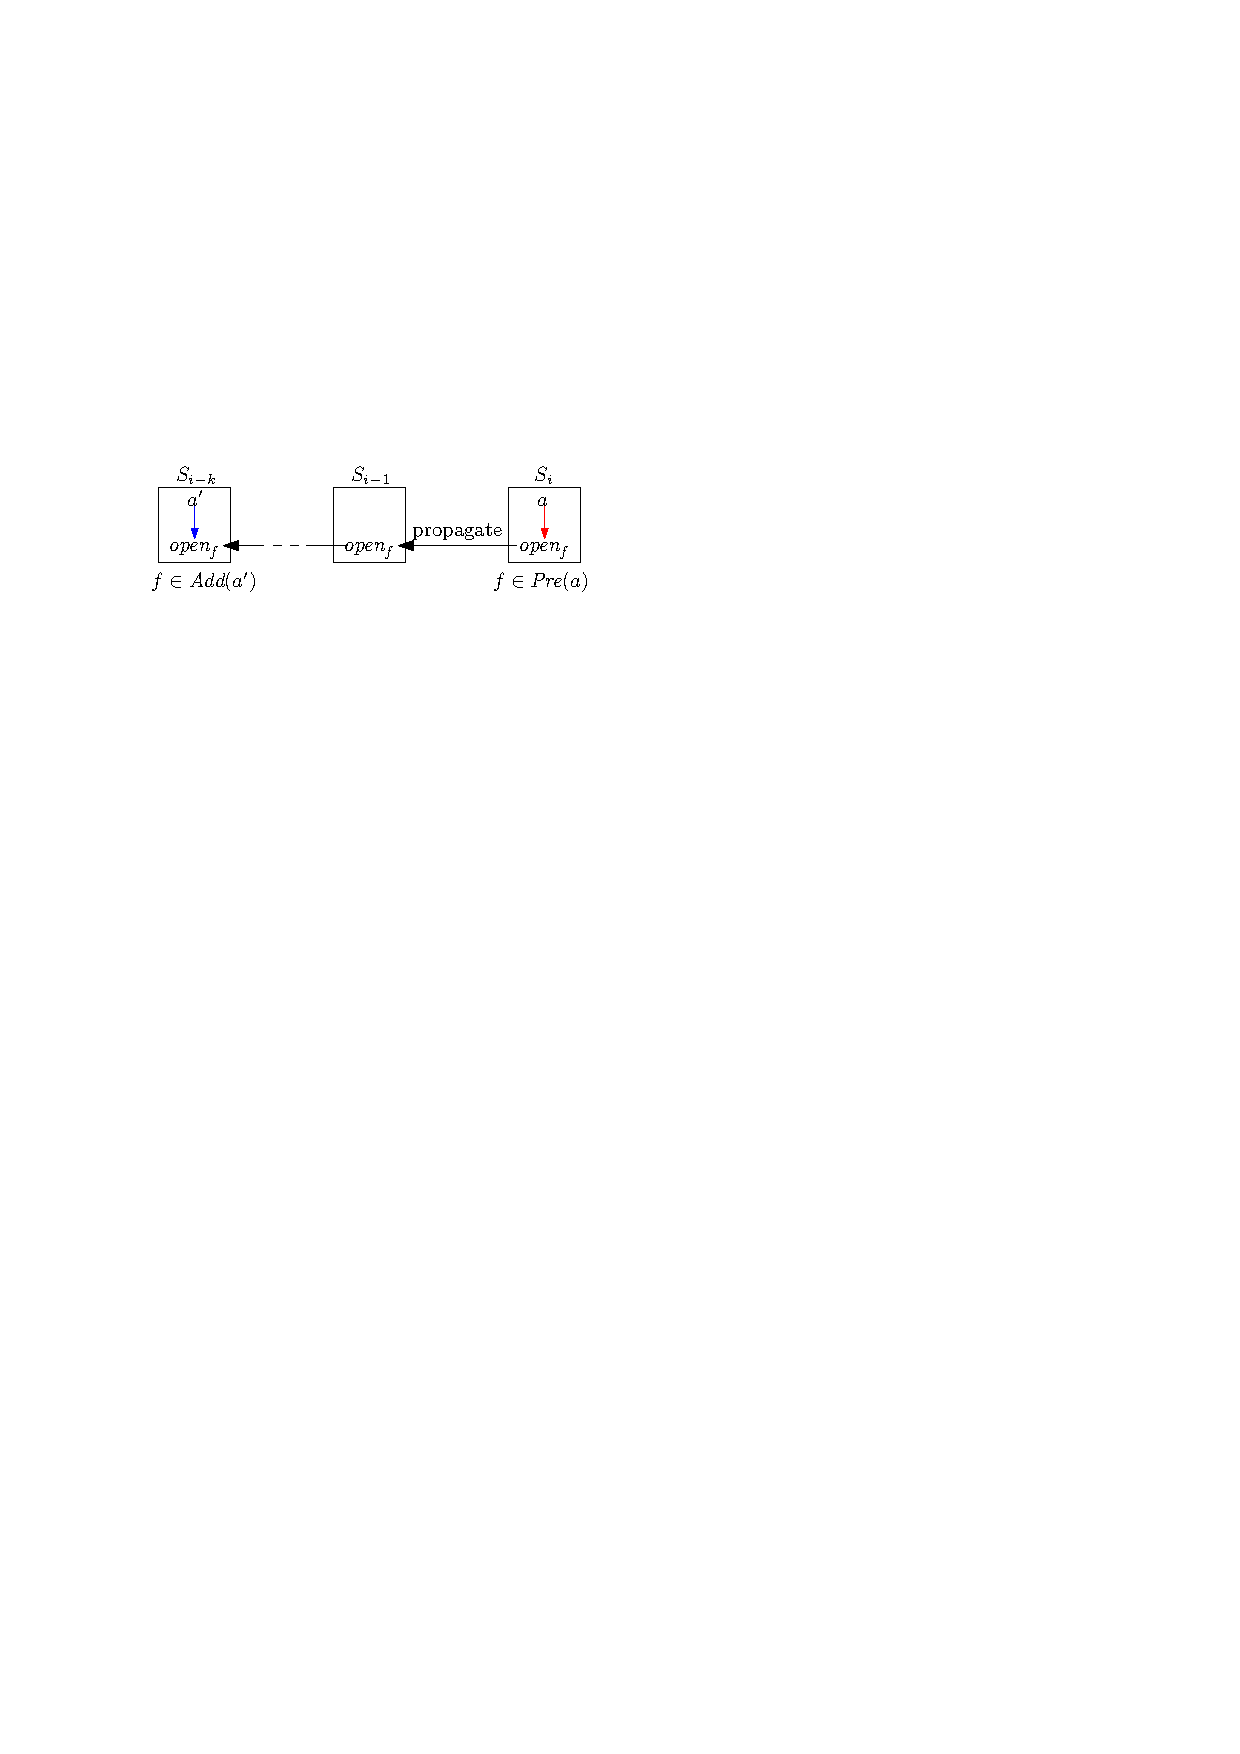
\includegraphics[width=.4\textwidth]{figures/transitions}
    \caption{Lien causal: $\b$ produit $\f$ pour $\a$.}
    \label{fig:causal-link}
\end{figure}

Nous définissons l'ensemble des variables ``open'', noté $\openSet$, comme $\openSet = \{\openSingle{\f} ~|~ \f \in \F \}$. Chaque action étant considérée comme une variable propositionnelle, nous définissons un ensemble de variables propositionnelles $\X$, donné par $\X = \A \cup \openSet$.


\paragraph*{Quantificateurs}

%In a CTE formula, we want to select two consecutive steps in order to define transitions (Figure~\ref{fig:plantree}).
Pour chaque profondeur $i$ de l'arbre, $\X_i$ dénote une copie de l'ensemble des variables $\X$. Il existe une seule variable $\a_{i}\in X_{i}$ pour chaque action utilisée pour déterminer la dernière transition dans le plan et une seule variable $\open{\f}{i}\in X_{i}$ pour chaque fluent utilisée pour déterminer si $\f$ est une condition ouverte. A la même profondeur~$i$, la valeur de ces variables dépend du n\oe ud (correspondant à une étape du plan) sélectionné par les valeurs des variables universelles de branchement supérieures $b_{i+1}\ldots b_{\depth}$.

\begin{small}
\[
\begin{matrix}
\displaystyle \bigexists_{\a \in \A} \a_{\depth}. \bigexists_{\f\in \F} \open{\f}{\depth}.%\\
\displaystyle {\bigforall b_{\depth}.}\\
\displaystyle \bigexists_{\a \in \A} \a_{\depth-1}. \bigexists_{\f\in \F} \open{\f}{\depth-1}.%\\
\displaystyle {\bigforall b_{\depth-1}.}\\
\displaystyle \dots\\ 
%\dots
\displaystyle \bigexists_{\a \in \A} \a_{1}. \bigexists_{\f\in \F} \open{\f}{1}.%\\
\displaystyle {\bigforall b_{1}.}%\\
\displaystyle \bigexists_{\a \in \A} \a_{0}. \bigexists_{\f\in \F} \open{\f}{0}.
\end{matrix}
\]
\end{small}\\

%Dans ce qui suit, un \textit{n\oe ud} désigne maintenant un n\oe ud qui n'est pas une feuille. % et $\depth$ est la profondeur de l'arbre.
%Le prédécesseur d'un n\oe ud au niveau $i$ est la feuille la plus à droite du sous-arbre gauche. Le successeur d'un noeud au niveau $i$ est la feuille la plus à gauche du sous-arbre droit.
%Afin de sélectionner ces transitions, nous introduisons l'opérateur feuille-vers-n\oe ud $\leftselect{i}$ défini comme:
%%\begin{scriptsize}
%\[\leftselect{i} \equiv \neg b_{i} \wedge \BigforallTwo{j=1}{i-1} b_{j}.\]
%%\end{scriptsize}
%Symétriquement, nous introduisons l'opérateur n\oe ud-vers-feuille $\rightselect{i}$ défini comme:
%%\begin{scriptsize}
%\[\rightselect{i} \equiv b_{i} \wedge \BigforallTwo{j=1}{i-1} \neg b_{j}.\]
%%\end{scriptsize}

\paragraph*{Conditions ouvertes}
%\displaystyle\mathop{\exists \a_{1}}_{\a \in \A} .\displaystyle\mathop{\exists \open{\f}{1}}_{\f\in \F} .\forall b_{1}. \displaystyle\mathop{\exists \a_{0}}_{\a \in \A} .\displaystyle\mathop{\exists \open{\f}{0}}_{\f\in \F} .\\
Si une action $\a$ est exécutée dans une étape du plan, alors chaque précondition de $\a$ doit être une condition ouverte à cette étape (c'est-à-dire qu'un lien causal est requis pour cette précondition).
%\begin{scriptsize}
\[ \BigforallTwo{i=0}{\depth} \Bigforall{\a \in \A} \left(\a_{i} \Rightarrow \Bigforall{\f\in \Cond{\a}} \open{\f}{i}\right) \]
%\end{scriptsize}

Dans la dernière étape du plan menant au but (c'est-à-dire la feuille la plus à droite de l'arbre), tous les fluents du but doivent être des conditions ouvertes ou ajoutées par des actions exécutées dans cette étape.
%must have its goal fluents ensured by an open condition that makes sure that this fluent will stay on until the end, or satisfied by the adding of this fluent by an action on the last state.
%\begin{scriptsize}
\[ \BigforallTwo{i=1}{\depth}b_{i} \Rightarrow \Bigforall{\f\in G} \left(\open{\f}{0} \vee \bigvee\limits_{\substack{\a \in \A \\ \f \in \Add{\a}}} \a_{0}\right) \]
%\end{scriptsize}

\paragraph*{Propagation et fermeture}

Aucune condition ne doit rester ouverte dans la première étape du plan (c'est-à-dire la feuille la plus à gauche de l'arbre) si elle n'est pas présente dans l'état initial.
%\begin{scriptsize}
\[ \BigforallTwo{i=1}{\depth}\neg b_{i} \Rightarrow \Bigforall{\f\in \F\setminus I} \neg \open{\f}{0} \]	
%\end{scriptsize}

Toute condition ouverte dans une étape doit, soit rester ouverte, soit être ajoutée (fermée) par une action à l'étape précédente.

%\begin{scriptsize}
\[ \BigforallTwo{i=1}{\depth} \Bigforall{\f\in \F} \left(\left(\open{\f}{i} \wedge \leftselect{i} \right) \Rightarrow \left(\open{\f}{0} \vee \bigvee\limits_{\substack{\a \in \A \\ \f \in \Add{\a}}} \a_{0}\right)\right) \]

\[ \BigforallTwo{i=1}{\depth}\Bigforall{\f\in \F}\left(\left(\open{\f}{0} \wedge \rightselect{i} \right) \Rightarrow \left(\open{\f}{i} \vee \bigvee\limits_{\substack{\a \in \A \\ \f \in \Add{\a}}} \a_{i}\right)\right)
\]
%\end{scriptsize}

 \paragraph*{Protection des conditions ouvertes}

Une condition ouverte dans une étape donnée ne peut pas être supprimée à l'étape précédente. Cela garantit de ne rompre aucun lien de causalité dans le plan.
%\begin{scriptsize}
\[ \BigforallTwo{i=1}{\depth} \Bigforall{\f\in \F}\left(\left(\open{\f}{i} \wedge \leftselect{i} \right) \Rightarrow \Bigforall{\a \in \A\\ \f \in \Del{\a}}\neg \a_{0}\right) \]
\[ \BigforallTwo{i=1}{\depth} \Bigforall{\f \in \F} \left(\left(\open{\f}{0} \wedge \rightselect{i} \right) \Rightarrow \Bigforall{\a \in \A \\ \f \in \Del{\a}}\neg \a_{i}\right) \]
%\end{scriptsize}

\paragraph*{Prévention des interactions négatives}

Si une action supprime un fluent qui est nécessaire ou est ajouté par une autre action, alors ces deux actions ne peuvent pas être exécutées toutes les deux dans une même étape.
%\begin{scriptsize}
\[ \BigforallTwo{i=0}{\depth} \Bigforall{\a \in \A} \Bigforall{\f\in \left(\Add{\a} \cup \Cond{\a}\right)} \Bigforall{\b \in \A \\ \a \neq \b \\ \f \in \Del{\b}}\left(\neg \a_{i} \vee \neg \b_{i}\right) \]
%\end{scriptsize}


%
% codage CTE-EFA
%
\subsubsection{Nouveau codage QBF dans les espaces d'états: CTE-EFA}

Dans ce codage, nous définissons l'ensemble des variables propositionnelles comme $\X = \A \cup \F$. Chaque étape est maintenant définie par une transition (comme dans CTE-OPEN) ainsi que par l'état résultant (valuation des fluents de $\F$). La formule est une adaptation au CTE des règles bien connues de codage SAT de \cite{KS92} basées sur des frame-axiomes explicatifs dans les espaces d'états.

\paragraph*{Quantificateurs}

A chaque profondeur $i$ de l'arbre, il existe une seule variable $\a_{i}$ pour chaque action utilisée pour déterminer la dernière transition dans le plan et une seule variable $\f_{i}$ pour chaque fluent utilisée pour déterminer l'état.
A la même profondeur $i$, les valeurs de ces variables dépendent du n\oe ud (correspondant à une transition dans le plan et à l'état résultant) sélectionné par les valeurs des variables universelles de branchement supérieures $b_{i+1}\ldots b_{\depth}$.

\begin{small}
\[
\begin{matrix}
\displaystyle \bigexists_{\a \in \A} \a_{\depth}. \bigexists_{\f\in \F} \f_{\depth}.%\\
\displaystyle {\bigforall b_{\depth}.}\\
\displaystyle \bigexists_{\a \in \A} \a_{\depth-1}. \bigexists_{\f\in \F} \f_{\depth-1}.%\\
\displaystyle {\bigforall b_{\depth-1}.}\\
\displaystyle \dots\\ 
%\dots
\displaystyle \bigexists_{\a \in \A} \a_{1}. \bigexists_{\f\in \F} \f_{1}.%\\
\displaystyle {\bigforall b_{1}.}%\\
\displaystyle \bigexists_{\a \in \A} \a_{0}. \bigexists_{\f\in \F} \f_{0}.
\end{matrix}
\]
\end{small}%\\

\paragraph*{But}

Dans l'état après la dernière transition du plan (c'est-à-dire la feuille la plus à droite de l'arbre), tous les fluents du but doivent être atteints.

%\begin{scriptsize}
\[ \BigforallTwo{i=1}{\depth} b_{i} \Rightarrow \Bigforall{\f\in G} {\f}_{0} \]	
%\end{scriptsize}

\paragraph*{Conditions et effets des actions}

Si une action $\a$ est exécutée dans une transition du plan, alors chaque effet de $\a$ se produit dans l'état résultant et chaque précondition de $\a$ est requise dans l'état précédent.
%\begin{scriptsize}
\[ \BigforallTwo{i=0}{\depth} \Bigforall{\a \in \A} \left(\a_{i} \Rightarrow \left( \Bigforall{\f\in \Add{\a}} \f_{i} \right) \wedge \left( \Bigforall{\f\in \Del{\a}} \neg \f_{i} \right) \right) \]
%\end{scriptsize}

%\begin{scriptsize}
\[ \BigforallTwo{i=1}{\depth} \Bigforall{\a\in \A}
\left(\a_{i} \wedge \leftselect{i} \Rightarrow \Bigforall{\f \in \Cond{\A}} \f_{0}\right)\]
\[\BigforallTwo{i=1}{\depth} \Bigforall{\a\in \A}
\left(\a_{0} \wedge \rightselect{i} \Rightarrow \Bigforall{\f \in \Cond{\A}} \f_{i}\right)\]
%\end{scriptsize}

De plus, une action qui n'a pas toutes ses préconditions dans l'état initial ne peut pas être exécutée dans la première transition du plan (c'est-à-dire la feuille la plus à gauche de l'arbre):

%\begin{scriptsize}
\[ \BigforallTwo{i=1}{\depth}\neg b_{i} \Rightarrow \Bigforall{\a\in \A\\ \Cond{\a} \not\subset I} \neg {\a}_{0} \]
%\end{scriptsize}

\paragraph*{Frame-axiomes explicatifs}

%{\color{blue}We only give here one of the four rules for explanatory frame axioms, the others being very similar. \color{red} Fred: j'ai ajouté les 4 règles + celles pour l'étape initiale}
Si la valeur d'un fluent change entre deux états consécutifs, alors une action qui produit cette modification est exécutée dans la transition du plan entre ces états.

\begin{small}
\[ \BigforallTwo{i=1}{\depth} \Bigforall{\f\in \F}
\left(\left(\neg\f_{0} \wedge \f_{i} \wedge \leftselect{i} \right) \Rightarrow \left(\bigvee\limits_{\substack{\a \in \A \\ \f \in \Add{\a}}} \a_{i}\right)\right)\]

\[ \BigforallTwo{i=1}{\depth} \Bigforall{\f\in \F}
\left(\left(\neg\f_{i} \wedge \f_{0} \wedge \rightselect{i} \right) \Rightarrow \left(\bigvee\limits_{\substack{\a \in \A \\ \f \in \Add{\a}}} \a_{0}\right)\right)\]
\end{small}

\begin{small}
\[ \BigforallTwo{i=1}{\depth} \Bigforall{\f\in \F}
\left(\left(\f_{0} \wedge \neg\f_{i} \wedge \leftselect{i} \right) \Rightarrow \left(\bigvee\limits_{\substack{\a \in \A \\ \f \in \Del{\a}}} \a_{i}\right)\right)\]
\[ \BigforallTwo{i=1}{\depth} \Bigforall{\f\in \F}
\left(\left(\f_{i} \wedge \neg\f_{0} \wedge \rightselect{i} \right) \Rightarrow \left(\bigvee\limits_{\substack{\a \in \A \\ \f \in \Del{\a}}} \a_{0}\right)\right)\]
\end{small}

Une règle supplémentaire est également requise pour décrire les frame-axiomes explicatifs pour la première transition du plan à partir de l'état initial (c'est-à-dire la feuille la plus à gauche de l'arbre):

%\begin{scriptsize}
\[ \Bigforall{\f\in \F\setminus I} \left(\left(\f_{0}\wedge \BigforallTwo{i=1}{\depth}\neg b_{i}\right) \Rightarrow \Bigexists{\a\in \A\\ \f\in\Add{\a}\\\Cond{\a} \subset I} {\a}_{0} \right) \]
\[ \Bigforall{\f\in I} \left(\left(\neg\f_{0}\wedge \BigforallTwo{i=1}{\depth}\neg b_{i}\right) \Rightarrow \Bigexists{\a\in \A\\ \f\in\Del{\a}\\\Cond{\a} \subset I} {\a}_{0} \right) \]
%\end{scriptsize}

\paragraph*{Prévention des interactions négatives}

Contrairement à CTE-NOOP et CTE-OPEN, les effets contradictoires sont déjà interdits par les règles précédentes (effets des actions).
Cette règle doit donc seulement empêcher les interactions entre les préconditions et les retraits des actions. Si une action supprime un fluent nécessaire à une autre action, ces deux actions ne peuvent pas être exécutées dans une même transition du plan.

%\begin{scriptsize}
\[ \BigforallTwo{i=0}{\depth} \Bigforall{\a \in \A} \Bigforall{\f\in \Cond{\a}} \Bigforall{\b \in \A \\ \a \neq \b \\ \f \in \Del{\b}}\left(\neg \a_{i} \vee \neg \b_{i}\right) \]
%\end{scriptsize}



%\subsection{Finding Minimal Plan Length}

%\begin{figure}[ht]
%\begin{center} \includegraphics[width=.45\textwidth]{images/dichotomie-1} \end{center}
%\caption{incremental search}
%\end{figure}






%%%%%%%%%%%%%%%%%%%%%%%%%%%%%
% PLANIFICATION SMT
%%%%%%%%%%%%%%%%%%%%%%%%%%%%%
\section{Planification temporelle par satisfaction de formules logiques}
%


%\subsection{Planification temporelle}
\subsection{Définitions préliminaires}

%Nous \'{e}tudions la planification temporelle propositionnelle dans un langage bas\'{e} sur les aspects temporels de PDDL2.1 \cite{DBLP:journals/jair/FoxL03}. 
Un fluent est une proposition atomique positive ou n\'{e}gative. Comme dans PDDL2.1, nous consid\'{e}rons que les changements des valeurs des fluents sont instantan\'{e}s mais que les conditions sur la valeur des fluents peuvent \^{e}tre impos\'{e}es sur un intervalle. Une action $\a$ est un quadruplet $\langle\cond{\a},\add{\a},\del{\a},\constr{a}\rangle$, o\`{u} l'ensemble des conditions $\cond{\a}$ est l'ensemble des fluents qui doivent \^{e}tre vrais pour que $\a$ soit ex\'{e}cut\'{e}e, l'ensemble des ajouts $\add{\a}$ est l'ensemble des fluents qui sont \'{e}tablis par $\a$, l'ensemble des retraits $\del{\a}$ est l'ensemble des fluents qui sont d\'{e}truits par $\a$, et l'ensemble de contraintes $\constr{a}$ est un ensemble de contraintes entre les temps relatifs des \'{e}v\'{e}nements qui se produisent pendant l'ex\'{e}cution de $\a$. Un \'{e}v\'{e}nement correspond \`{a} l'une des quatre possibilit\'{e}s: l'\'{e}tablissement ou la destruction d'un fluent par une action $\a$, ou le d\'{e}but ou la fin d'un intervalle sur lequel un fluent est requis par une action $\a$. Dans PDDL2.1, les \'{e}v\'{e}nements ne peuvent se produire qu'au d\'{e}but ou \`{a} la fin des actions, mais nous rel\^{a}chons cette hypoth\`{e}se de sorte que les \'{e}v\'{e}nements peuvent se produire \`{a} tout moment \`{a} condition que les contraintes $\constr{\a}$ soient satisfaites. Notons que $\add{\a} \cap \del{\a}$ peut \^{e}tre non vide. En effet, il n'est pas inhabituel pour une action durative d'\'{e}tablir un fluent au d\'{e}but de l'action et de le d\'{e}truire \`{a} sa fin. Nous pouvons \'{e}galement observer que la dur\'{e}e d'une action, le temps entre le premier et le dernier \'{e}v\'{e}nement de l'action, n'a pas besoin d'\^{e}tre explicitement stock\'{e}e.
%Nous représentons des actions non-instantanées par un rectangle. La durée d'une action est donnée entre crochets après le nom de l'action. Les conditions sont écrites au-dessus d'une action, et les effets ci-dessous. L'action CHARGE (m, c) représentée sur la figure 1 représente le chargement d'un lot de béton c dans un mélangeur m. Nous avons Cond (LOAD (m, c)) = {Fluid (c), Empty (m), At-factory (m)}. On peut voir sur la figure que le mélangeur doit être vide au début du chargement, alors que le béton doit être fluide et le malaxeur à l'usine pendant toute la durée du chargement. Nous avons Del (LOAD (m, c)) = {Empty (m)} et Add (LOAD (m, c) = {On (m, c)} Nous pouvons voir sur la figure que dès que le chargement commence, le mélangeur n'est plus vide et à la fin du chargement le mélangeur contient le béton.


Nous utilisons la notation $\a \rightarrow \f$ pour d\'{e}signer l'\'{e}v\'{e}nement que l'action $\a$ \'{e}tablit le fluent $\f$, $\a \rightarrow \neg\f$ pour d\'{e}signer l'\'{e}v\'{e}nement que $\a$ d\'{e}truit $\f$, et $\f \mid\rightarrow \a$ et $\f \rightarrow\mid \a$, respectivement, pour indiquer le d\'{e}but et la fin de l'intervalle sur lequel $\a$ requiert la condition $\f.$ Si $\f$ est d\'{e}j\`{a} vrai (respectivement, faux) lorsque l'\'{e}v\'{e}nement
$\a \rightarrow \f$ ($\a \rightarrow \neg\f$) se produit, nous consid\'{e}rons toujours que $\a$ \'{e}tablit (d\'{e}truit) $\f$. Un plan temporel peut contenir plusieurs instances de la m\^{e}me action, mais %puisque la plupart des plans temporels étudiés dans cet article contiennent au plus un exemple de chaque action, 
par simplicit\'{e} de notation, nous ferons seulement la distinction entre actions et instances d'action si cela est absolument n\'{e}cessaire. Nous utilisons la notation $\tau(e)$ pour repr\'{e}senter l'instant dans un plan o\`{u} un \'{e}v\'{e}nement $e$ se produit.
Pour une action donn\'{e}e (ou une instance d'action) $a$, $\events{\a}$ repr\'{e}sente les diff\'{e}rents \'{e}v\'{e}nements qui constituent sa d\'{e}finition, \`{a} savoir $\a \rightarrow \f$ pour tout $\f$ dans $\add{\a}$, $\a \rightarrow \neg\f$ pour tout $\f$ dans $\del{\a}$, $\f \mid\rightarrow \a$ et $\f \rightarrow\mid \a$ pour tout $\f$ dans $\cond{a}$. La d\'{e}finition d'une action $\a$ inclut les contraintes $\constr{a}$ sur les instants relatifs aux \'{e}v\'{e}nements dans $\events{\a}$. %Par exemple, la structure interne de l'action de longueur fixe LOAD (m, c) représentée sur la figure 1 est définie par des contraintes telles que
%τ (Fluide (c) → | CHARGE (m, c)) - τ (Fluide (c) | → CHARGE (m, c)) = 5
%τ (LOAD (m, c) → On (m, c)) - τ (Fluide (c) → | LOAD (m, c)) = 0
Comme dans PDDL2.1, nous consid\'{e}rons que la dur\'{e}e entre \'{e}v\'{e}nements dans $\events{\a}$ n'est pas n\'{e}cessairement fixe et que $\constr{\a}$ est un ensemble de contraintes d'intervalle sur des paires d'\'{e}v\'{e}nements, tels que
$\tau(\f \rightarrow\mid \a) - \tau(\f \mid\rightarrow \a) \in [\alpha,\beta]$ pour des constantes $\alpha,\beta$. Nous utilisons $[\alpha_{\a}(e_1, e_2), \beta_{\a}(e_1, e_2)]$ pour d\'{e}signer l'intervalle de valeurs possibles pour la distance relative entre les \'{e}v\'{e}nements $e_1$, $e_2$ de l'action $\a$. Une dur\'{e}e fixe entre les \'{e}v\'{e}nements $e_1,e_2 \in \events{\a}$ peut, bien s\^{u}r, \^{e}tre mod\'{e}lis\'{e}e en d\'{e}finissant $\alpha_{\a}(e_1, e_2)=\beta_{\a}(e_1, e_2)$. De m\^{e}me, l'absence de contrainte peut \^{e}tre mod\'{e}lis\'{e}e par l'intervalle $[-\infty,+\infty]$. Nous introduisons maintenant deux contraintes fondamentales que tous les plans temporels doivent satisfaire :
\begin{itemize}
\item les \emph{contraintes inh\'{e}rentes} \`{a} l'ensemble des instances d'action $\A$ : pour toute $\a\in\A$, $\a$ satisfait $\constr{a}$, c'est-\`{a}-dire pour toutes les paires d'\'{e}v\'{e}nements $e_1,e_2\in \events{\a}$ nous avons $\tau(e_1) - \tau(e_2) \in [\alpha_\a(e_1,e_2),\beta_\a(e_1,e_2)]$ ;
\item les \emph{contraintes d'effets contradictoires} sur l'ensemble des instances d'action $\A$ : pour toutes $\a_i,\a_j \in\A$, pour tout fluent positif $\f \in \del{\a_i} \cap \add{\a_j}$ nous avons $\tau(\a_i \rightarrow \neg\f) \neq \tau(\a_j \rightarrow \f)$.
\end{itemize}

Les contraintes inh\'{e}rentes d\'{e}finissent la structure interne de chaque instance d'action, alors que les contraintes d'effets contradictoires assurent que la valeur de v\'{e}rit\'{e} de chaque fluent ne soit jamais ind\'{e}finie lors de l'ex\'{e}cution d'un plan temporel. %Par exemple, si un plan contient une instance $\a$ de l'action LOAD (m, c) montrée à la figure 1 et une instance b d'une autre action CLEAN (m) avec Empty (m) ∈ Add (CLEAN (m)), alors le plan temporel doit satisfaire la contrainte d'effets contradictoires
%τ (a → ¬EMPTY (m)) ≠ τ (b → EMPTY (m)).

\begin{definition}
Un probl\`{e}me de planification temporelle $\langle \I, \A, \G \rangle$ consiste en un ensemble d'actions $\A,$ un \'{e}tat initial $\I$ et un but $\G$, o\`{u} $\I$ et $\G$ sont des ensembles de fluents.
\end{definition}
\paragraph*{Notation} Si $\A$ est un ensemble d'instances d'actions, alors $\events{\A}$ est l'union des ensembles $\events{\a}$ (pour toutes les instances d'action $a\in \A$).

\begin{definition}\label{def:plan-temporel}
$P = \langle \A, \tau \rangle$, o\`{u} $\A$ est un ensemble fini d'instances d'actions $\{a_1,\ldots, a_n\}$ et $\tau$ est une fonction \`{a} valeurs r\'{e}elles sur $\events{\A}$, est un plan temporel pour le probl\`{e}me $\langle \I , \A^{\prime}, \G \rangle$ si
\begin{enumerate}
\item[(1)] $\A \subseteq \A^{\prime}$, et
\item[(2)] $P$ v\'{e}rifie les contraintes inh\'{e}rentes et contradictoires sur $\A$;
\end{enumerate}
et lorsque $P$ est ex\'{e}cut\'{e} (c'est-\`{a}-dire que les fluents sont \'{e}tablis ou d\'{e}truits aux instants donn\'{e}s par $\tau$) \`{a} partir de l'\'{e}tat initial $\I$:
\begin{enumerate}
\item[(3)] pour toute $a_i \in \A$, chaque $\f \in \cond{a_i}$ est vrai lorsqu'il est requis, et
\item[(4)] tous les fluents $g \in \G$ sont vrais \`{a} la fin de l'ex\'{e}cution de $P$.
\item[(5)] $P$ est robuste sous des changements infinit\'{e}simaux dans les temps de d\'{e}marrage des actions.
\end{enumerate}
\end{definition}

Les \'{e}v\'{e}nements sont instantan\'{e}s, alors que les actions ont non seulement une dur\'{e}e mais celle-ci peut aussi \^{e}tre de longueur variable. Ainsi, un plan temporel $P$ ne planifie pas directement ses instances d'action mais planifie tous les \'{e}v\'{e}nements dans ses instances d'actions.
La condition (5) de la d\'{e}finition~\ref{def:plan-temporel} signifie que nous interdisons les plans qui exigent une synchronisation parfaite entre diff\'{e}rentes actions. % montrent comment 
Cette condition peut \^{e}tre impos\'{e}e dans PDDL2.1 \cite{DBLP:conf/ecai/FoxLH04}. Nous exigeons que dans tous les plans, les fluents soient \'{e}tablis strictement avant le d\'{e}but de l'intervalle sur lequel ils sont requis. La seule exception \`{a} cette r\`{e}gle est lorsqu'un fluent $\f$ est \'{e}tabli et requis par la m\^{e}me action $\a$. Nous permettons la possibilit\'{e} d'une parfaite synchronisation au sein d'une action, ce qui signifie que nous pouvons avoir $\tau(\a\rightarrow\f)=\tau(\f\mid\rightarrow\a)$.
De m\^{e}me, les fluents ne peuvent \^{e}tre d\'{e}truits qu'apr\`{e}s la fin de l'intervalle sur lequel ils sont requis. La seule exception \`{a} cette regle est quand un fluent $\f$ est requis et d\'{e}truit par une action $\a$, auquel cas on peut avoir $\tau(\f\rightarrow\mid\a)=\tau(\a\rightarrow\neg\f)$. %Par exemple, le fluide Empty (m) est simultanément requis et détruit par l'action LOAD (m, c) représentée sur la figure 1.

\begin{definition}
Un probl\`{e}me de planification temporelle $\langle \I, \A, \G \rangle$ est positif s'il n'y a pas de fluents n\'{e}gatifs dans les conditions d'actions ni dans le but $\G$.
\end{definition}

Dans cet article, nous ne consid\`{e}rerons que des probl\`{e}mes de planification temporelle positifs $\langle \I, \A, \G \rangle$. Il est bien connu que tout probl\`{e}me de planification peut \^{e}tre transform\'{e} en un probl\`{e}me positif \'{e}quivalent en temps lin\'{e}aire par l'introduction, pour chaque fluent positif $\f$, d'un nouveau fluent pour remplacer les occurrences de $\neg\f$ dans les conditions d'actions \cite{DBLP:books/daglib/0014222}. %Il est important de noter, cependant, que cette transformation peut ne pas conserver d'autres propri\'{e}t\'{e}s de l'instance. 
En supposant que tous les probl\`{e}mes sont positifs, $\G$ et $\cond{\a}$ (pour toute action $\a$) sont compos\'{e}s de fluents positifs. Par convention, $\add{\a}$ et $\del{a}$ sont aussi compos\'{e}s exclusivement de fluents positifs. L'\'{e}tat initial $\I$, cependant, peut contenir des fluents n\'{e}gatifs.
%Pour simplifier la pr\'{e}sentation, nous supposons dans cet article que l'ensemble des actions A a subi l'op\'{e}ration de filtrage consistant \`{a} \'{e}liminer les actions $\a$ de $\A$ qui ne peuvent \^{e}tre ex\'{e}cut\'{e}es puisque $\cond{\a}$ n'est pas un sous-ensemble de $\I\cup\add{\a}$.


%\subsubsection{Codage SAT pour la planification classique}
%Dans cette section, nous consid\'{e}rons la planification classique comme restriction de la planification temporelle d\'{e}crite dans la section pr\'{e}c\'{e}dente. Un probl\`{e}me de planification positif est donc ici un triplet $\langle \I , \A, \G \rangle$ tel que toutes les actions de $\A$ sont instantan\'{e}es (c'est-\`{a}-dire $\forall \a\in\A, \forall e_1,e_2\in \events{\a}, \tau(e_1)=\tau(e_2)$). De plus, nous consid\'{e}rons pour tout plan $P = \langle \A, \tau \rangle$, que $\tau$ est une fonction \`{a} valeurs enti\`{e}res de $\events{\A}$ dans $N=\{1,\ldots,n\}$ l'ensemble ordonn\'{e} des index d'\'{e}tapes de $P$.


%
% codage-open-sat (old)
%
%





%\begin{frame}
%\begin{figure}\label{steps}
% \hspace{0.8em}\xymatrix@C=1pc@R=1pc{
%  Init \ar[r] & \fbox{S$_{1}$} \ar[r]  & \fbox{S$_{2}$} \ar[r] & \fbox{S$_{3}$} \ar[r] & \fbox{S$_{4}$} \ar[r] & \fbox{S$_{5}$} \ar[r] & \fbox{S$_{6}$} \ar[r] & \fbox{S$_{7}$} \ar[r] & Goal \\
%  }
%  \vspace{2em}
%   \hspace{0.8em}\xymatrix@C=0.2pc@R=1pc{
%   & & & & & \fbox{S$_{4}$} \ar@{.}[lld] \ar@{.}[rrd] \ar@/^1pc/[rdd] \\
%   & & & \fbox{S$_{2}$} \ar[rd] & & & & \fbox{S$_{6}$} \ar[rd] \\
%  Init \ar[rr] & & \fbox{S$_{1}$} \ar[ru]  & & \fbox{S$_{3}$} \ar@/^1pc/[ruu] & & \fbox{S$_{5}$} \ar[ru] & & \fbox{S$_{7}$} \ar[rr] & & Goal \\
%  }
%\caption{Transitions of an 8-steps plan in SAT/SMT encoding and QBF compact tree encoding (CTE)}
%\end{figure}
%\end{frame}


\subsection{Codages SMT de référence pour la planification temporelle}
%

%
% SMT TLP-GP
%

\fred{Règles de TLP-GP (Maris, Régnier 2008)}

\paragraph*{Etat initial et But}

Les nœuds d'actions factices Init (produisant l'état initial) et Goal (nécessitant le but) sont tous deux vrais.

\paragraph*{Production des préconditions par liens causaux}

Si une action $\a_{i}$ est active dans le plan à une étape $i$, alors pour chacune de ses préconditions $\f$, il existe au moins un lien causal (noté $\Link{\b_{j}}{\f}{\a_{i}}$) d'une action $\b_{j}$, qui produit cette précondition à l'étape $j$, vers $\a_{i}$.

\[ \BigforallTwo{i=1}{i=\length} \Bigforall{\a\in\A} \left( \a_{i} \Rightarrow \Bigforall{\f\in\Cond{\a}} \BigexistsTwo{j=1}{j=i}\Bigexists{\b\in\A\\\f\in\Add{\b}} \Link{\b_{j}}{\f}{\a_{i}} \right)
\]

\paragraph*{Activation des actions et ordre partiel}

S’il existe un lien causal entre une action $\b_{j}$ qui produit une précondition $\f$ pour une action $\a_{i}$, alors $\b_{j}$ et $\a_{i}$ sont actives dans le plan et l’instant où $\b_{j}$ produit certainement $\f$ est antérieur ou égal à l’instant où $\a_{j}$ commence à nécessiter $\f$.

\[
\begin{matrix}
\BigforallTwo{i=1}{i=\length} \BigforallTwo{j=1}{i=j} \Bigforall{(\a,\b)\in\A^{2}} \Bigforall{\f\in\left(\Cond{\a}\cap\Add{\b}\right)}\\ \left( \Link{\b_{j}}{\f}{\a_{i}} \Rightarrow \left( \b_{j} \wedge \a_{i} \wedge \tau(\b_{j}\rightarrow\f) \leq \tau(\f\mid\rightarrow\a_{i}) \right) \right)
\end{matrix}
\]

\paragraph*{Protection des liens causaux}

Si un lien causal assure la protection d’un fluent $\f$ et qu'une action qui le détruit est active dans le plan, alors l’intervalle temporel correspondant au lien causal et l’intervalle temporel correspondant à l’activation de $\neg \f$ (la destruction de $\f$) par l’action sont disjoints.

\[
\begin{matrix}
\BigforallTwo{i=1}{i=\length} \BigforallTwo{j=1}{i=j} \BigforallTwo{k=1}{k=\length} \Bigforall{(\a,\b)\in\A^{2}} \Bigforall{\f\in\left(\Cond{\a}\cap\Add{\b}\right)} \Bigforall{\c\in\A\\\f\in\Del{\c}}\\ \left( \Link{\b_{j}}{\f}{\a_{i}} \wedge \c_{k} \Rightarrow \left( \begin{matrix} \tau(\c_{k}\rightarrow\neg\f) < \tau(\b_{j}\rightarrow\f)\\ \vee \tau(\f\rightarrow\mid\a_{i}) < \tau(\c_{k}\rightarrow\neg\f) \end{matrix} \right) \right)
\end{matrix}
\]

\paragraph*{Prévention des interactions négatives}

Si deux actions produisant respectivement une proposition p et sa négation sont actives dans le plan, alors les intervalles temporels correspondants à l’activation de p et à l’activation de ¬p sont disjoints.

\[
\begin{matrix}
\BigforallTwo{i=1}{i=\length} \BigforallTwo{j=1}{j=\length} \Bigforall{(\a,\b)\in\A^{2}} \Bigforall{\f\in\left(\Add{\a}\cap\Del{\b}\right)}\\ \left( \a_{i} \wedge \b_{j} \Rightarrow \left( \begin{matrix} \tau(\a_{i}\rightarrow\neg\f) < \tau(\b_{j}\rightarrow\f)%\\ \vee \tau(\f\rightarrow\mid\a_{i}) < \tau(\c_{k}\rightarrow\neg\f) 
\end{matrix} \right) \right)
\end{matrix}
\]

\paragraph*{Bornes inférieure et supérieure}

L’instant initial où les propositions de l’état initial sont vraies est antérieur à tous les instants de début des préconditions des actions du plan. L’instant final où les propositions du but sont vraies est postérieur à tous les instants de fin des effets des actions du plan.
\fred{à ajouter}


\subsection{Nouveau codage SMT pour la planification temporelle}

Nous introduisons une adaptation SMT du codage SAT bas\'{e} sur les conditions ouvertes que nous avons introduit dans la section \fred{ajout référence} pour la planification classique. Ici, les actions ne sont plus instantan\'{e}es et des contraintes sur les instants $\tau(e)$ auxquels se produisent des \'{e}v\'{e}nements $e\in\events{\A}$ doivent explicitement \^{e}tre ajout\'{e}es.


Consid\'{e}rons donc maintenant un probl\`{e}me de planification temporelle positif $\langle \I, \A, \G \rangle$.
Pour chaque instance d'action $\a$ et chaque fluent $\f\in \cond{a}$, nous introduisons deux variables $\tau_{s}(\textit{open}_{f})$ et $\tau_{e}(\textit{open}_{f})$ qui nous permettent de d\'{e}finir un intervalle temporel de protection de lien causal depuis l'\'{e}tat initial ou une \'{e}tape contenant une action qui produit $\f$ vers une \'{e}tape qui contient l'instance d'action $\a$. Durant cet intervalle temporel, aucune action ne pourra d\'{e}truire $\f$.


%%\paragraph*{Planning with Continuous Time}
%%%\begin{alertblock}{Definition}
%%For each action $a = \langle \cond{a},\add{a},\del{a} \rangle$:
%%\begin{itemize}
%%  \item $\forall f\in \cond{a}$ we define:
%%    \begin{itemize}
%%      \item $[\tau(f\mid\rightarrow a);\tau(f\rightarrow\mid a)]$
%%%      \item $open_{f}$
%%      \item $[\tau_{s}(\textit{open}_{f});\tau_{e}(\textit{open}_{f})]$
%%    \end{itemize}
%%  \item $\forall f\in \add{a}$ we define $[\tau(a\mid\rightarrow f);\tau(a\rightarrow\mid f)]$
%%  \item $\forall f\in \del{a}$ we define $[\tau(a\mid\rightarrow \neg f);\tau(a\rightarrow\mid \neg f)]$
%%\end{itemize}
%%%\begin{itemize}
%%%  \item $A \wedge (f\in \cond{A}) \rightarrow f_{~[\tau(f\mid\rightarrow A);\tau(f\rightarrow\mid A)]}$
%%%  \item $A \wedge (f\in \add{A}) \rightarrow f_{~[\tau(A\mid\rightarrow f);\tau(A\rightarrow\mid f)]}$
%%%  \item $A \wedge (f\in \del{A}) \rightarrow \neg f_{~[\tau(A\mid\rightarrow \neg f);\tau(A\rightarrow\mid \neg f)]}$
%%%\end{itemize}
%%%\end{alertblock}


%\begin{frame}{SMT Temporal Planning}
%Classical planning: PSPACE-complete~\cite{DBLP:journals/ai/Bylander94}.
%\end{frame}


\paragraph*{Conditions ouvertes} Si une action $\a$ est ex\'{e}cut\'{e}e dans une \'{e}tape du plan, alors chaque condition de $\a$ doit \^{e}tre une condition ouverte \`{a} cette \'{e}tape (c'est-\`{a}-dire qu'un lien causal est requis pour cette condition). De plus, le d\'{e}but de l'intervalle sur lequel cette condition est requise se trouve dans l'intervalle de protection du lien causal $[\tau_{s}(\textit{open}_{f});\tau_{e}(\textit{open}_{f})]$.

\begin{small}
\begin{multline*}
~\\[-3em]
\BigforallTwo{i=1}{\length}\bigwedge\limits_{\substack{\mathbf{\a}\in \mathbf{\A}}}\hfill\\
\left(\mathbf{\a}_{\mathbf{i}} \Rightarrow \bigwedge\limits_{\substack{\mathbf{f}\in \cond{\mathbf{\a}}}}\begin{pmatrix}open_{\mathbf{\f},\mathbf{i}}\hfill\\ \wedge \left(\tau(\mathbf{\f}\mid\rightarrow\mathbf{\a}_\mathbf{i}) \geq \tau_{s}(open_{\mathbf{f},\mathbf{i}})\right)\hfill\\
 \wedge \left(\tau(\mathbf{\f}\mid\rightarrow\mathbf{\a}_\mathbf{i}) \leq \tau_{e}(open_{\mathbf{\f},\mathbf{i}})\right)\end{pmatrix}\right)\hfill\\[-2em]
%%%
\end{multline*}
\end{small}

Dans la derni\`{e}re \'{e}tape du plan menant au but tous les fluents du but doivent \^{e}tre des conditions ouvertes ou ajout\'{e}es par des actions ex\'{e}cut\'{e}es dans cette \'{e}tape. Dans le cas o\`{u} une action $\a$ ajoute une condition ouverte $\f$, le d\'{e}but de l'intervalle de protection du lien causal correspondant est fix\'{e} \`{a} l'instant o\`{u} $\a$ produit $\f$.

\begin{small}
\begin{multline*}
~\\[-3em]
\bigwedge\limits_{\substack{\mathbf{\f}\in \mathbf{\G}}}\begin{pmatrix}open_{\mathbf{\f},\mathbf{\length}} \hfill\\\vee \bigvee\limits_{\substack{\mathbf{\a}\in \mathbf{\A}\\\mathbf{\f} \in \add{\mathbf{\a}}}}\begin{pmatrix}\mathbf{\a}_{\mathbf{\length}}\hfill\\
 \wedge \left(\tau(\mathbf{\a}_\mathbf{\length}\rightarrow \mathbf{\f}) = \tau_{s}(open_{\mathbf{\f},\mathbf{\length}})\right)\hfill\\
  \wedge \left(\tau_{\textit{Goal}} = \tau_{e}(open_{\mathbf{f},\mathbf{\length}})\right)\hfill\end{pmatrix}\end{pmatrix}\hfill\\[-2em]
%
%\bigwedge\limits_{\substack{\mathbf{f}\in \mathbf{G}}}\left(\tau_{\textit{Goal}} = \tau_{e}(open_{\mathbf{f},\mathbf{length}})\right)\hfill\
%%%
\end{multline*}
\end{small}


\paragraph*{Propagation et fermeture}

Aucune condition ne doit rester ouverte dans la premi\`{e}re \'{e}tape du plan si elle n'est pas fournie dans l'\'{e}tat initial.

\begin{small}
\begin{multline*}
~\\[-3em]
\bigwedge\limits_{\substack{\mathbf{\f}\in \mathbf{\F}\setminus \mathbf{\I}}}\neg open_{\mathbf{\f},1}\hfill\\[-2em]
%%%
\end{multline*}
\end{small}

Si une condition ouverte est fournie par l'\'{e}tat initial, alors le d\'{e}but de l'intervalle de protection du lien causal correspondant est fix\'{e} \`{a} l'instant initial $\tau_{\textit{Init}}$.

\begin{small}
\begin{multline*}
~\\[-3em]
\bigwedge\limits_{\substack{\mathbf{\f}\in \mathbf{\I}}}\left(open_{\mathbf{\f},1} \Rightarrow \left(\tau_{\textit{Init}} = \tau_{s}(open_{\mathbf{\f},1})\right)\right)\hfill\\[-2em]
%%%
\end{multline*}
\end{small}

Toute condition ouverte $\f$ dans une \'{e}tape doit \`{a} l'\'{e}tape pr\'{e}c\'{e}dente : (1) soit rester ouverte et dans ce cas l'intervalle de protection du lien causal correspondant reste le m\^{e}me pour ces deux \'{e}tapes, (2) soit \^{e}tre ajout\'{e}e (ferm\'{e}e) par une instance d'action $\a$ et dans ce cas le d\'{e}but de l'intervalle de protection du lien causal est fix\'{e} \`{a} l'instant de production de $\f$ par $\a$.

\begin{small}
\begin{multline*}
~\\[-3em]
\bigwedge\limits_{\substack{\mathbf{i}\in [2..\mathbf{\length}]}}~\bigwedge\limits_{\substack{\mathbf{\f}\in \mathbf{\F}}}\hfill\\
\begin{pmatrix}open_{\mathbf{\f},\mathbf{i}} \Rightarrow\hfill\\ \begin{pmatrix}\begin{pmatrix}open_{\mathbf{\f},\mathbf{i} - 1}\hfill\\ \wedge %\begin{pmatrix}
\left(\tau_{s}(open_{\mathbf{\f},\mathbf{i} - 1}) = \tau_{s}(open_{\mathbf{\f},\mathbf{i}})\right)\hfill\\
 \wedge \left(\tau_{e}(open_{\mathbf{f},\mathbf{i} - 1}) = \tau_{e}(open_{\mathbf{\f},\mathbf{i}})
 \right)\end{pmatrix}\hfill\\
 \vee \bigvee\limits_{\substack{\mathbf{\a}\in \mathbf{\A}\\\mathbf{\f} \in \add{\mathbf{\a}}}}\left(\mathbf{\a}_{\mathbf{i} - 1} \wedge \left(\tau(\mathbf{\a}_{\mathbf{i} - 1}\rightarrow \mathbf{\f}) = \tau_{s}(open_{\mathbf{\f},\mathbf{i}})\right)\right)\hfill\\
 \end{pmatrix}\end{pmatrix}\\[-2em]
%%%
\end{multline*}
\end{small}


\paragraph*{Protection des conditions ouvertes}

Une condition ouverte dans une \'{e}tape donn\'{e}e ne peut pas \^{e}tre supprim\'{e}e \`{a} l'int\'{e}rieur de l'intervalle de protection du lien causal correspondant $[\tau_{s}(\textit{open}_{f});\tau_{e}(\textit{open}_{f})]$. Cela garantit de ne rompre aucun lien de causalit\'{e} dans le plan.

\begin{small}
\begin{multline*}
~\\[-3em]
\bigwedge\limits_{\substack{\mathbf{i}\in [1..\mathbf{\length}]\\ \mathbf{j}\in [1..\mathbf{\length}]}}%~\bigwedge\limits_{\substack{\mathbf{j}\in [1..\mathbf{\length}]}}
~\bigwedge\limits_{\substack{\mathbf{\f}\in \mathbf{\F}}}~\bigwedge\limits_{\substack{\mathbf{\a}\in \mathbf{\A}\\\mathbf{\f} \in \del{\mathbf{\a}}}}\hfill\\
\left(\left(open_{\mathbf{\f},\mathbf{i}} \wedge \mathbf{\a}_{\mathbf{j}}\right) \Rightarrow \begin{pmatrix}\left(\tau(\mathbf{\a}_\mathbf{j}\rightarrow \neg \mathbf{\f}) < \tau_{s}(open_{\mathbf{\f},\mathbf{i}})\right)\hfill\\
 \vee \left(\tau_{e}(open_{\mathbf{\f},\mathbf{i}}) < \tau(\mathbf{\a}_\mathbf{j}\rightarrow \neg \mathbf{\f})\right)\end{pmatrix}\right)\hfill\\[-2em]
%%%
\end{multline*}
\end{small}


\paragraph*{Pr\'{e}vention des interactions n\'{e}gatives}

Si une action $\b$ supprime, \`{a} un instant $\tau(\b\rightarrow\neg\f)$, un fluent $\f$ qui est ajout\'{e} par une autre action $\a$ \`{a} un instant $\tau(\a\rightarrow\f)$, alors ces deux instants sont diff\'{e}rents.

\begin{small}
\begin{multline*}
~\\[-3em]
\bigwedge\limits_{\substack{\mathbf{i}\in [1..\mathbf{\length}]\\ \mathbf{j}\in [1..\mathbf{\length}]}}%~\bigwedge\limits_{\substack{\mathbf{j}\in [1..\mathbf{\length}]}}
~\bigwedge\limits_{\substack{\mathbf{\a}\in \mathbf{\A}}}~\bigwedge\limits_{\substack{\mathbf{\f}\in \add{\mathbf{\a}}}}~\bigwedge\limits_{\substack{\mathbf{\b}\in \mathbf{\A}\\((\mathbf{i} \neq \mathbf{j}) \vee (\mathbf{\a} \neq \mathbf{\b})) \wedge \mathbf{\f} \in \del{\mathbf{\b}}}}\hfill\\
\left(\left(\mathbf{\a}_{\mathbf{i}} \wedge \mathbf{\b}_{\mathbf{j}}\right) \Rightarrow %\begin{pmatrix}
\left(\tau(\mathbf{\a}_\mathbf{i}\rightarrow \mathbf{\f}) \neq \tau(\mathbf{\b}_\mathbf{j}\rightarrow \neg \mathbf{\f})\right)\hfill%\\
% \vee \left(\tau(\mathbf{\b}_\mathbf{j}\rightarrow\mid \neg \mathbf{\f}) < \tau(\mathbf{\a}_\mathbf{i}\mid\rightarrow \mathbf{\f})\right)
%\end{pmatrix}
\right)\hfill\\[-2em]
%%%%%%%%%%
\end{multline*}
\end{small}

De m\^{e}me, si une action $\b$ supprime, \`{a} un instant $\tau(\b\rightarrow\neg\f)$, un fluent $\f$ qui est n\'{e}cessaire \`{a} une autre action $\a$ sur un intervalle temporel $[\tau(\f\mid\rightarrow\a), \tau(\f\rightarrow\mid\a)]$, alors cet instant ne peut \^{e}tre contenu dans cet intervalle.

\begin{small}
\begin{multline*}
~\\[-3em]
\bigwedge\limits_{\substack{\mathbf{i}\in [1..\mathbf{\length}]\\ \mathbf{j}\in [1..\mathbf{\length}]}}%~\bigwedge\limits_{\substack{\mathbf{j}\in [1..\mathbf{\length}]}}
~\bigwedge\limits_{\substack{\mathbf{\a}\in \mathbf{\A}}}~\bigwedge\limits_{\substack{\mathbf{\f}\in \cond{\mathbf{\a}}}}~\bigwedge\limits_{\substack{\mathbf{\b}\in \mathbf{\A}\\((\mathbf{i} \neq \mathbf{j}) \vee (\mathbf{\a} \neq \mathbf{\b})) \wedge \mathbf{\f} \in \del{\mathbf{\b}}}}\hfill\\
\left(\left(\mathbf{\a}_{\mathbf{i}} \wedge \mathbf{\b}_{\mathbf{j}}\right) \Rightarrow \begin{pmatrix}\left(\tau(\mathbf{f}\rightarrow\mid\mathbf{\a}_\mathbf{i}) < \tau(\mathbf{\b}_\mathbf{j}\rightarrow \neg \mathbf{\f})\right)\hfill\\
 \vee \left(\tau(\mathbf{\b}_\mathbf{j}\rightarrow \neg \mathbf{\f}) < \tau(\mathbf{\f}\mid\rightarrow\mathbf{\a}_\mathbf{i})\right)\end{pmatrix}\right)\hfill\\[-2em]
%%%
\end{multline*}
\end{small}


%\paragraph*{SMT Encoding: bound the plan with Init and Goal states}
\paragraph*{Bornes du plan temporel}
Enfin, nous devons ajouter une contrainte pour maintenir le plan dans un intervalle de temps born\'{e} par l'\'{e}tape initiale qui produit l'\'{e}tat initial $\I$ et l'\'{e}tape finale qui n\'{e}cessite tous les fluents du but $\G$.
\begin{small}
\begin{multline*}
~\\[-2em]
\bigwedge\limits_{\substack{\mathbf{i}\in [1..\mathbf{\length}]}}~\bigwedge\limits_{\substack{\mathbf{\a}\in \mathbf{\A}}}\hfill\\
\left(\mathbf{\a}_{\mathbf{i}} \Rightarrow \begin{pmatrix}\bigwedge\limits_{\substack{\mathbf{\f}\in \cond{\mathbf{\a}}}} \begin{pmatrix}\left(\tau_{\textit{Init}} \leq \tau(\mathbf{\f}\mid\rightarrow\mathbf{\a}_\mathbf{i}) \right)\hfill\\%
 \wedge \left(\tau_{\textit{Goal}} \geq \tau(\mathbf{f}\rightarrow\mid\mathbf{\a}_\mathbf{i})\right) \end{pmatrix}\hfill\\
 \wedge \bigwedge\limits_{\substack{\mathbf{\f}\in \add{\mathbf{\a}}}} \begin{pmatrix}\left(\tau_{\textit{Init}} \leq \tau(\mathbf{\a}_\mathbf{i}\rightarrow \mathbf{\f}) \right)\hfill\\%
 \wedge \left(\tau_{\textit{Goal}} \geq \tau(\mathbf{\a}_\mathbf{i}\rightarrow \mathbf{f})\right) \end{pmatrix}\hfill\\
 \wedge \bigwedge\limits_{\substack{\mathbf{\f}\in \del{\mathbf{\a}}}} \begin{pmatrix}\left(\tau_{\textit{Init}} \leq \tau(\mathbf{\a}_\mathbf{i}\rightarrow \neg \mathbf{\f}) \right)\hfill\\%
 \wedge \left(\tau_{\textit{Goal}} \geq \tau(\mathbf{\a}_\mathbf{i}\rightarrow \neg \mathbf{\f})\right) \end{pmatrix} \end{pmatrix}\right)\\[1em]
 %%%
% \bigwedge\limits_{\substack{\mathbf{i}\in [1..\mathbf{length}]}}\bigwedge\limits_{\substack{\mathbf{A}\in \mathbf{O}}} \left(\neg \mathbf{A}_{\mathbf{i}} \Rightarrow \left(t_{\mathbf{A},\mathbf{i}} = -1\right)\right)\hfill\\
\end{multline*}
\end{small}





%\section{Jeux avec QBF}
%\fred{ajouter le jeu de Nim (JIAF2017), partie adaptation du solveur QBF pour résolution interactive à mettre dans le chapitre sur TouIST}


%\section{Extension aux logiques dynamiques}

\section{Conclusion}



%%%%%%%%%%%%%%%%%%%%%
% CHAPITRE : TouIST
%%%%%%%%%%%%%%%%%%%%%
\chapter{Traduction automatique avec TouIST}
%\section{État de l'art, les solveurs du moment}
%\subsection{Introduction des logiques SAT, SMT, QBF}
%\subsection{Le principe des solveurs SAT, SMT, QBF}

\section{Historique de TouIST}

\subsection{Genèse de \satoulouse}

Lors de la conférence ICTTL'2011, l'équipe (\citeauthor{GaScSt2011}) avait présenté l'outil \satoulouse\ \cite{GaScSt2011}, dédié à la logique propositionnelle, dont les principales fonctions étaient (1) d'offrir un langage logique de haut niveau pour exprimer succinctement des formules complexes et (2) de trouver des modèles à ces formules en utilisant un solveur SAT performant.

Bien sûr, il existe de nombreux outils logiques comme des prouveurs, assistants de preuves, éditeurs de tables de vérité\ldots disponibles sur Internet ; PROLOG aurait même pu être utilisé, mais aucun de ces outils ne correspond aux exigences de l'équipe, à savoir :
\begin{itemize}
\item l'outil doit être très facile à installer et à utiliser, sans syntaxe complexe ;
\item le prouveur peut être utilisé comme une boîte noire sans savoir comment il fonctionne ;
\item  aucune mise en forme normale,  aucun ordonnancement de clauses, ou aucune coupure PROLOG ne doivent être requis ;
\item seulement une petite connaissance en logique devrait être nécessaire.
\end{itemize} 

L'équipe ne trouvant aucun outil existant satisfaisant ces exigences, il a été décidé de développer un nouvel logiciel en 2010. L'objectif était de développer une interface qui permettrait d'utiliser confortablement un prouveur SAT (à savoir SAT4J \cite{DBLP:journals/jsat/BerreP10}). L'outil, appelé \satoulouse\, est décrit dans \cite{GaScSt2011}. À travers cet outil, l'utilisateur pouvait expérimenter par lui-même l'idée qu'un langage logique n'est pas seulement descriptif mais peut aussi conduire à des calculs qui résolvent des problèmes de la vie réelle. En particulier, dans le domaine éducatif, \satoulouse donnait l'occasion lors de cours avec des étudiants de L1 et L2 de résoudre des Sudokus en quelques lignes, ainsi que beaucoup d'autres problèmes combinatoires (emplois du temps, coloration de carte, circuits électroniques\ldots).\

Voici les principales facilités qu'offraient \satoulouse\ :
\begin{itemize}
\item les formules entrées n'ont pas besoin d'être sous forme clausale et des connecteurs arbitraires peuvent être utilisés, la mise sous forme normale est faite dynamiquement pendant la saisie au clavier de l'utilisateur ;
\item des facilités d'utilisation de grandes conjonctions ou disjonctions sont offertes comme dans :
\end{itemize}
  \[\bigwedge_{i\in\{1..9\}}
  \bigvee_{j\in\{1..9\}}\bigwedge_{n\in\{1..9\}}\bigwedge_{m\in\{1..9\},m\neq
    n}(p_{i,j,n}\rightarrow \lnot p_{i,j,m})\]
\begin{itemize}
\item démarrer le solveur consiste à cliquer sur un bouton ;
\item l'outil affiche un modèle dans la syntaxe de la formule entrée.
\end{itemize}
Ainsi, il est possible de mettre à disposition à l'utilisateur la puissance de la logique propositionnelle avec pour seul pré-requis la formalisation de phrases en logique ainsi que les notions de validité et satisfiabilité pour résoudre, par exemple, des Sudokus.\

L'avantage de ce type d'outil tient au fait qu'un même solveur SAT peut être utilisé pour résoudre de nombreux autres problèmes combinatoires aussi facilement que pour le Sudoku : ils suffit de formaliser les contraintes. Ces problèmes vont de la gestion des emplois du temps, la coloration de cartes ou même le stockage de produits chimiques qui doivent être stockés dans des salles identiques/contiguës/non-contiguës en fonction de leur degré de compatibilité.

\subsection{Limites de \satoulouse\ et genèse de \touist}
Mais pendant ces années, nous avons remarqué quelques limitations dommageables de \satoulouse\ : de nombreux bugs, des défauts dans l'interface, le manque de modularité (si l'on souhaite changer le prouveur SAT utilisé), l'ambiguïté et les limites de son langage, etc.

Par exemple, des problèmes impliquant des contraintes de cardinalité, comme les règles du jeu de Takuzu\footnote{Connu aussi sous le nom de Binero.\\ \url{http://fr.wikipedia.org/wiki/Takuzu}} qui nécessitent de compter des 0 et des 1, ne peuvent être facilement formalisés : il manque des fonctionnalités permettant d'exprimer des choses comme ``exactement 5 parmi 10 propositions sont vraies''. 

De plus, \satoulouse\ n'offre pas la possibilité de parcourir l'ensemble des modèles fournis par le solveur, il en retourne seulement un.






\color{red}
Les leçons tirées de trois années d'utilisation de \satoulouse\ sont que beaucoup des étudiants en informatique ont clairement pris conscience que la logique avait des applications réelles en ce qui concerne la résolution de problèmes, et beaucoup d'entre-eux ont acquis une capacité dans la formalisation de problèmes. Mais les défauts de \satoulouse\ rendent le déboggage vraiment difficile, d'une part parce qu'un seul modèle est affiché et en raison de la façon dont ce modèle est affiché, et d'autre part à cause des faibles capacités d'édition dont il dispose. En outre, seuls des problèmes combinatoires purs peuvent être traités, ce qui limite lourdement la prétention de résolution d'une large gamme de problèmes par \satoulouse\ concernant les problèmes du monde réel.

Un autre inconvénient de \satoulouse, pas nécessairement lié à l'enseignement de la logique, est son incapacité à être utilisé à partir de la ligne de commande : les travaux de recherche nécessitent d'automatiser l'utilisation des outils pour les utiliser dans le cadre de benchmarks.

Enfin, l'extension à des théories plus riches est également quelque chose qui peut intéresser les chercheurs, les ingénieurs ou les étudiants de cycles supérieurs. \satoulouse\ n'est certainement pas adapté pour la satisfiabilité modulo théories ou pour résoudre des problèmes de planification alors que la même architecture logicielle pourrait être utilisée en changeant juste le solveur.


Il y a quelques mois, nous avons commencé à développer un nouveau logiciel qui comblerait ces lacunes et remplirait nos attentes. Nous l'avons appelé \touist\ qui signifie TOUlouse Integrated Satisfiability Tool et doit être prononcé ``twist''.
 \touist\ est bien sûr à la disposition du public pour téléchargement à partir du site suivant :
\begin{center}\url{ https://github.com/touist/touist }\end{center}
\color{black}

Pour résumer, voici quelques fonctionnalités offertes par \touist\ et que \satoulouse\ ne propose pas :
\begin{itemize}
\item définition d'ensembles de domaines : $\bigwedge_{i\in A}$ vs. $\bigwedge_{i\in\{Paris,London,Roma,Madrid\}}$
\item liaisons multiples sur les indices: $\bigwedge_{i\in A,j\in B}$ vs. $\bigwedge_{i\in \cdots} \bigwedge_{j\in \cdots}$
\item calculs riches sur les indices ainsi que sur les ensembles de domaines: $\bigwedge_{i\in (A\cup (B \cap C))}$
\item primitives de contraintes de cardinalité intégrées: ``auMoins'' (resp. ``auPlus'', ``exactement'') \emph{tant} de valeurs sont vraies parmi \emph{ces valeurs}
\item les prédicats peuvent également être des variables définies sur des ensembles de domaines: $\bigwedge_{X\in \{A,B\},i\in \{1,2\}} X(i)$ vs. $\bigwedge_{i\in \{1,2\}} (A(i)\AND B(i))$
\item littéraux spéciaux définissant des contraintes entre nombres entiers ou réels : ($x+y\leq z$)
\item parcours facile des modèles successivement calculés par les solveurs
\item expressions régulières permettant un filtrage des littéraux pertinents
\item possibilité d'utiliser le logiciel en ligne de commande et/ou batch
\item nombreuses fonctionnalités d'édition et améliorations
\end{itemize}

\subsection{Vue d'ensemble de \touist}\label{sec:sat_interface}


\touist\ est composé de trois modules, mais l'utilisateur standard ne verra que l'un d'entre eux : l'interface. Dans la suite nous insistons principalement sur cette dernière plut\^ot que sur le traducteur et le solveur. L'architecture globale est illustr\'{e}e par la figure~\ref{fig:architectureTouisT}: 

\begin{figure}[htbp]
\centering
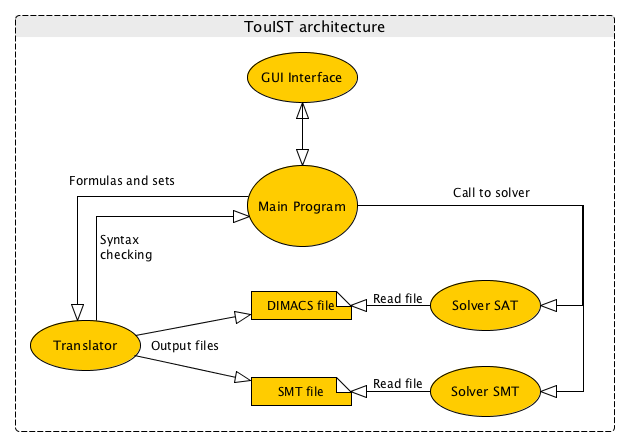
\includegraphics[scale=0.37]{Pictures/DiagTouist.png}
  \caption{Architecture de TouIST}
  \label{fig:architectureTouisT}
\end{figure}

Avec \touist\ , on accède à un éditeur puissant et convivial pour éditer des formules logiques complexes et des contraintes variées comme :

$$\bigwedge_{i \in \{1..9\}} (P_i \IMPL Q_{i+1})$$

qui abrège confortablement :\\ 

$(P_1 \Rightarrow Q_2) \AND (P_2 \IMPL Q_3) \AND \ldots (P_9\IMPL Q_{10})$. 
\\

Une fois qu'un ensemble de formules a été donné à l'interface, sa satisfiabilité peut \^etre vérifiée : l'interface peut l'envoyer au prouveur qui retourne un modèle, affich\'{e} comme le montre la figure \ref{fig:ExampleOfAModel} si un tel mod\`{e}le existe. Ensuite par l'intermédiaire de l'interface, l'utilisateur peut par exemple demander d'autres modèles (bouton ``Next'' de l'interface). Contrairement à \satoulouse\ qui aurait nécessité de modifier les formules pour interdire le modèle et de relancer le solveur, \touist\ conserve une instance du solveur en attente, ce qui permet d'obtenir les modèles suivants bien plus rapidement.

\begin{figure}[htbp]
\centering
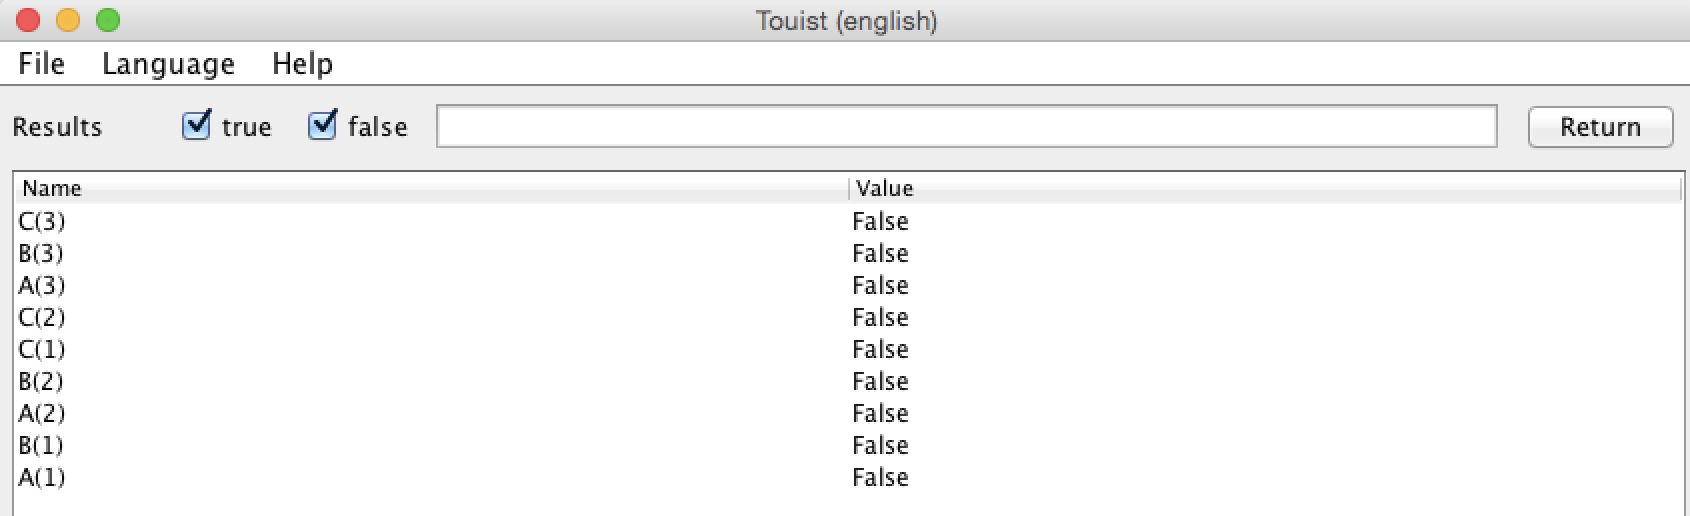
\includegraphics[scale=0.27]{Pictures/ExampleOfAModel.png}
  \caption{Affichage de mod\`{e}le}
  \label{fig:ExampleOfAModel}
\end{figure}

Les mod\`{e}les renvoy\'{e}s par le solveur sont totaux : une valeur est affect\'{e}e \`{a} chacune des variables apparaissant dans les formules envoy\'{e}es au solveur. L'utilisateur peut s\'{e}lectionner uniquement les propositions vraies ou les propositions fausses. Il peut \'{e}galement s\'{e}lectionner des sous-ensembles de variables en tapant une expression r\'{e}guli\`{e}re pour les filtrer.


\section{L'entrée : le langage de \touist}

\subsection{Aperçu de l'expressivité de \nameTool\label{sec:sat_tobedone}}

\paragraph{Ensembles de domaines}
Avec le temps, nous avons remarqué que nous avions souvent besoin d'écrire des choses comme :
$$\begin{aligned}\bigwedge_{i \in \{1..9\}} \bigwedge_{j \in \{1..9\}}\bigwedge_{ m\in \{A,B,C,D,E,F,G,H,I\}} \hspace{2cm}\\ \left( P_{i,j,m}\IMPL \bigwedge_{n \in \{A,B,C,D,E,F,G,H,I\}|m\neq n}\NOT P_{i,j,n}\right)\end{aligned}$$
Si on lit $P_{i,j,m}$ comme  ``il y a la lettre $m$ dans la case $(i,j)$'' d'une grille $9\times 9$, la formule ci-dessus exprime qu'il y a \emph{au plus} une lettre parmi `A' ... `I' dans chaque case. 

Ces ensembles $\{1..9\}$ et $\{A,B,C,D,E,F,G,H,I\}$ sont des \emph{ensembles de domaines}, et avec \nameTool\ l'utilisateur peut définir autant d'ensembles de domaines qu'il le souhaite, par exemple :

\begin{verbatim}
  $N=[1..9]
  $L=[A,B,C,D,E,F,G,H,I]
\end{verbatim}

et ainsi écrire la formule précédente comme :
$$\bigwedge_{i \in N} \bigwedge_{j \in N}\bigwedge_{ m\in L}P_{i,j,m}\IMPL \bigwedge_{n \in L|m\neq n}\NOT P_{i,j,n}$$
De plus, les opérations usuelles sur les ensembles ($\cup$, $\cap$, $\setminus$, \ldots) peuvent être utilisées pour définir d'autres ensembles.


\paragraph{Formules propositionnelles}

Les formules de \nameTool\ sont basées sur des variables propositionnelles (qui peuvent être indicées) et les opérateurs logiques usuels ($\AND$, $\OR$, $\IMPL$, $\NOT$, $\IFF$). Ainsi on peut taper des formules usuelles simples comme $Pluie \IMPL Nuages$. Mais en plus, nous fournissons des opérateurs logiques de haut niveau qui permettent d'exprimer des assertions complexes dans une forme très compacte.

\paragraph{Conjonctions et disjonctions généralisées}
Elles permettent d'exprimer des conjonctions et des disjonctions sur des formules contenant des paramètres qui varient, par exemple :
\begin{itemize}
\item $ \bigwedge_{i \in N} P_i$, o\`u $N$ est l'ensemble de domaine défini précédemment.\\
  Elle représente la conjonction
  $P_1 \AND P_2 \AND \ldots \AND P_9$. 
\item $\bigvee_{i \in E} P_i$.
\end{itemize}

Bien s\^ur, ces opérateurs peuvent être imbriqués comme dans :
$$\bigwedge_{i \in N} \bigwedge_{j \in N}\bigvee_{ m\in L}P_{i,j,m}$$

qui indique que dans chaque cellule se trouve au moins une lettre.


\paragraph{Contraintes de cardinalité}
Il s'agissait de l'un des sujets "laissé pour le futur" de \cite{GaScSt2011}.
Ces opérateurs logiques moins classiques sont disponibles dans \nameTool\ : il permettent de réduire drastiquement la taille de certaines formules, ce sont : $\atM{}{}$, $\atL{}{}$ et $\exact{}{}$.\\ L'exemple suivant décrit leur signification :
\begin{itemize}
\item $\atM{i \in N}{2} P_i$ représente ``pour au plus deux valeurs de $i \in N$ $P(i)$ est vraie'';
\item $\atL{i \in N}{2} P_i$ représente ``pour au moins deux valeurs de $i \in N$ $P(i)$ est vraie'';
\item $\exact{i \in N}{2} P_i$ représente ``pour exactement deux valeurs de $i \in N$ $P(i)$ est vraie''.
\end{itemize}
La disjonction généralisée est en fait un cas particulier de ceci (au moins une est vraie), la conjonction aussi (au plus 0 est fausse), et le ou exclusif peut être vu comme exactement une parmi deux est vraie. \\
Rappelons qu'avec des opérateurs logiques classiques et avec $N$ contenant 9 éléments, $\atM{i \in N}{3} P_i$ devrait nécessiter une formule contenant 84 propositions $P_i$ puisque cela revient à choisir 3 parmi 9 ce qui donne $\binom{9}{3}$ possibilités, et ni $\bigwedge$ ni $\bigvee$ n'aideraient beaucoup. 

\paragraph{Contraintes et calculs sur des indices}

Souvent, nous avons besoin d'ajouter des contraintes sur les indices, par exemple :
$$\bigwedge_{i \in E } \bigwedge_{j \in E  | i \neq j}P_{i,j}$$
qui signifie que $P_{i,j}$ est vraie lorsque $i\neq j$. 

Il s'agissait de la seule contrainte disponible dans \satoulouse, maintenant dans \nameTool\ la gamme de possibilités à été largement enrichie. Les contraintes peuvent inclure des opérateurs usuels de comparaison comme $<$, $>$, $\leq$, $\geq$, $\neq$, $=$ et ces comparaisons peuvent s'appliquer non seulement aux indices, mais aussi à toute expression arithmétique impliquant des indices et $+$, $-$, $*$, $/$, $\mod$, $\sqrt{\phantom{x}}$. 

Exprimer une phrase comme ``chaque case $(i,j)$ contient un nombre qui n'est pas égal à $i+j$'' donnera :
$$\bigwedge_{i \in N } \bigwedge_{j \in N} \bigvee_{k \in N|k\neq i+j} P_{i,j,k}$$
Bien s\^ur, \emph{toutes ces phrases} pourraient être exprimées avec les opérateurs logiques usuels bruts, mais ceci serait un travail fastidieux. Néanmoins, les étudiants doivent savoir ce qui est derrière la scène, et qu'une telle formule est l'abréviation de quelque chose comme :
$$P_{1,1,1}\vee P_{1,1,3}\vee P_{1,1,4}\ldots P_{1,2,1}\vee P_{1,2,2}\vee P_{1,2,4}\vee \ldots $$
qui est très long et terne.



\subsection{Détails du langage}

\subsubsection{Langage d'entrée vs. langage d'affichage}

Les formules que nous avons vues précédemment sont écrites dans le \emph{langage d'affichage} (style \LaTeX), mais tous ces symboles ne sont pas disponibles sur les claviers, ainsi pour écrire les formules et ensembles de domaines, l'utilisateur utilisera le \emph{langage d'entrée}.
Par exemple, la formule précédente avec l'ensemble associé $N$ sera tapée (les variables sont pr\'{e}fix\'{e}es par \$) :
\begin{verbatim}
bigand $i,$j in $N,$N:
  bigor $k in $N when $k != $i+$j:
    P($i,$j,$k)
  end
end
\end{verbatim}
Mais \nameTool\ les affiche immédiatement en style \LaTeX\ comme on peut le voir dans le panneau droit montr\'{e} sur la figure \ref{fig:LatexDisplay}.
La d\'{e}finition de l'ensemble $N$ est faite dans l'onglet ``Ensembles''.

\begin{figure*}[htbp]
\centering
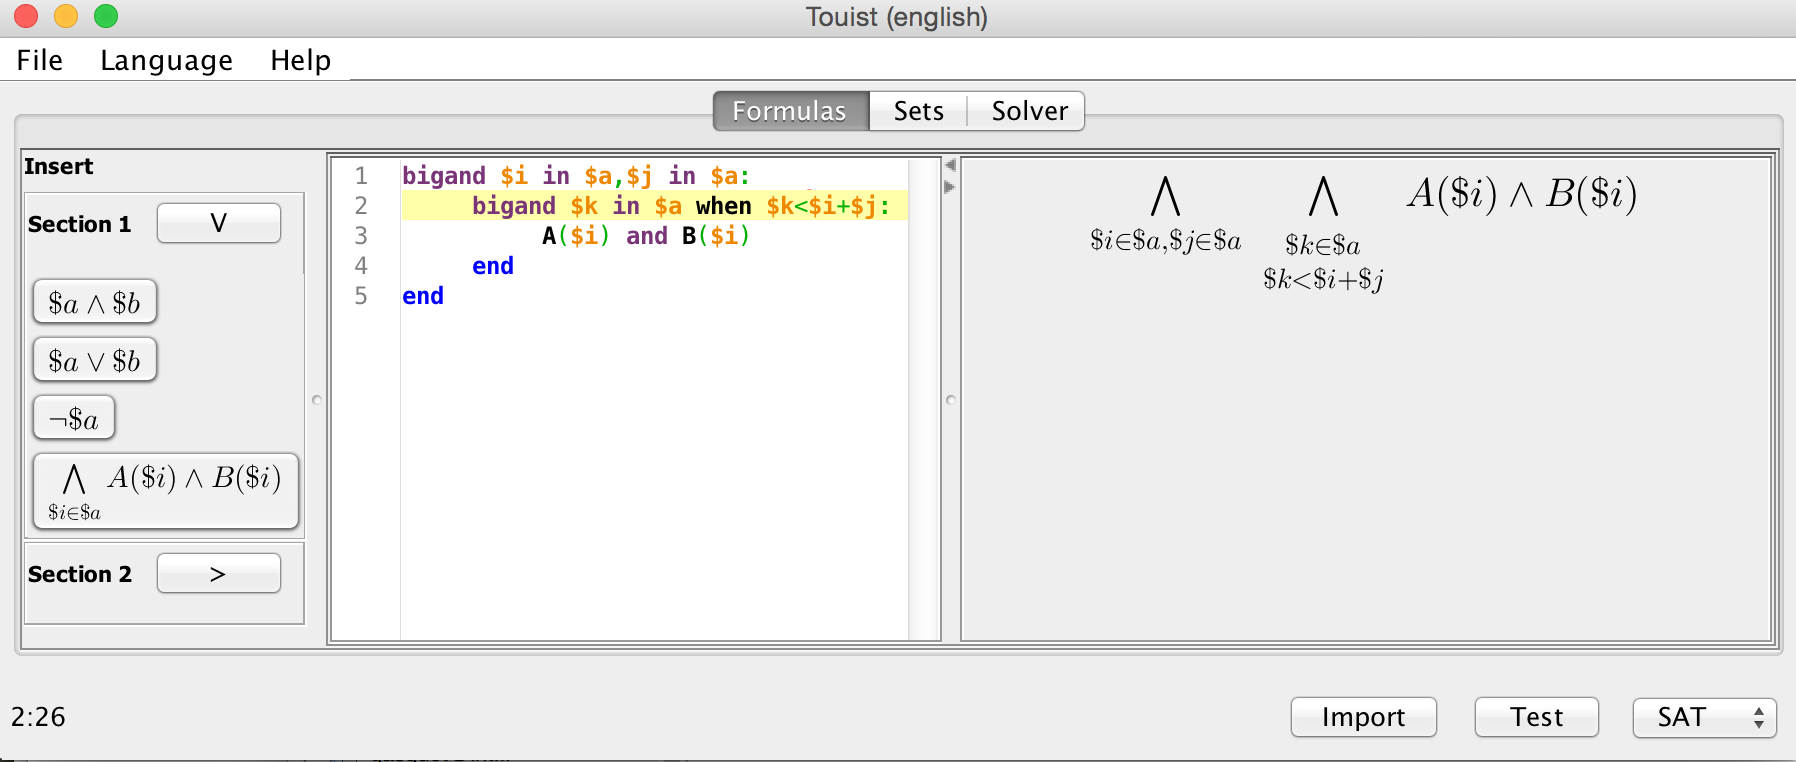
\includegraphics[scale=0.45]{Pictures/LatexDisplay.png}
  \caption{Affichage en style \LaTeX}
  \label{fig:LatexDisplay}
\end{figure*}


En outre, les formules peuvent être tapées à la main dans la fenêtre d'édition, ou introduites dans une sorte d'éditeur dirigé par la syntaxe, en raffinant progressivement l'arbre syntaxique, ou encore elles peuvent être importées à partir d'un fichier externe.





%\begin{figure*}[ht]
%  \centering
%  \includegraphics[scale=.4]{touist1.png}
%  \caption{Interface de TouIST}
%  \label{fig:touist}
%\end{figure*}



%\chapter{Language reference}\label{sec-language-reference}%mdk%mdk

Cette section présente les fonctionnalités liées au langage développé pendant la thèse.

\subsection{Structure d'un fichier {\scshape TouIST} file}\label{sec-structure-of-a-touist-file}%mdk%mdk
\begin{mdpre}%mdk
\noindent{\mdcolor{purple}\textless{}touist-file\textgreater{}}~::=~{\mdcolor{purple}\textless{}assign\textgreater{}}~{\mdcolor{purple}\textless{}touist-file\textgreater{}}\\
~~~~~~~~~~~~~~~~\textbar{}~{\mdcolor{purple}\textless{}formula\textgreater{}}~{\mdcolor{purple}\textless{}touist-file\textgreater{}}\\
~~~~~~~~~~~~~~~~\textbar{}~EOF%mdk
\end{mdpre}\noindent Un fichier {\scshape TouIST} est  whitespace-separated\footnote{\noindent A whitespace is a space, tab or newline.%mdk
\label{fn-whitespace}%mdk%mdk
} list of
assignments and formulas. Assignments are global and can be interleaved
with formulas as long as they are not nested in formulas (for local
variables, you can use \mdcode{{\mdcolor{navy}let}}; see Sec.~\ref{let-binding}). Comments begin
with "\mdcode{{\mdcolor{darkgreen};;}}". Two backslashes (\mdcode{\textbackslash{}\textbackslash{}}) in a formula will produce a new
line in the latex view.

\noindent\textbf{Note}.
The whitespace-separated list of formulas is actually going to be
converted to a conjunction; it avoids many intermediate \mdcode{and}.
\textbf{Warning:} each formula in this list is going to be put in
parentheses:%mdk
\begin{mdpre}%mdk
\noindent a~or~b\\
c~=\textgreater{}~a%mdk
\end{mdpre}\noindent will be translated to
\begin{mdpre}%mdk
\noindent(a~or~b)~and~(c~=\textgreater{}~a)%mdk
\end{mdpre}\label{newline-and-note}%mdk%mdk

\subsection{Variables}\label{sec-variables}%mdk%mdk

\noindent First, we describe what a variable is. Then, we detail how to assign
variables (with global or local assignments).%mdk

\subsubsection{Syntax of a variable}\label{sec-syntax-of-a-variable}%mdk%mdk
\begin{mdpre}%mdk
\noindent{\mdcolor{purple}\textless{}expr\textgreater{}}~::=~{\mdcolor{purple}\textless{}int\textgreater{}}\textbar{}{\mdcolor{purple}\textless{}float\textgreater{}}\textbar{}{\mdcolor{purple}\textless{}prop\textgreater{}}\textbar{}{\mdcolor{purple}\textless{}bool\textgreater{}}\textbar{}{\mdcolor{purple}\textless{}set\textgreater{}}\\
~~~~\textbar{}~"""{\mdcolor{purple}\textless{}formula-simple\textgreater{}}"""~{\mdcolor{darkgreen}\textless{}-~quoted~formula,~since~TouIST~\textgreater{}=~3.5.1}\\
{\mdcolor{purple}\textless{}var\textgreater{}}~::=~"\$"~TERM~~~~~~~~~~~~~~~~~~~~~~~~~~~~{\mdcolor{darkgreen}\textless{}-~simple-var}\\
~~~~\textbar{}~"\$"~TERM~"("~{\mdcolor{purple}\textless{}comma-list(\textless{}expr\textgreater{})\textgreater{}}~")"~~~{\mdcolor{darkgreen}\textless{}-~tuple-var}%mdk
\end{mdpre}
\begin{mddefinitions}%mdk

\mddefterm{\noindent{\bfseries Simple variable (\textquotedblleft{}simple-var\textquotedblright{})}}%mdk

\begin{mdbmarginx}{}{}{}{1.5em}%mdk
\begin{mddefdata}%mdk
A simple variable is of the form \mdcode{{\mdcolor{purple}\$my\_var}}. In a formula, a simple
variable is always expected to be a proposition or a
\mdref{quoted-formulas}{quoted formula}. In an expression, a simple
variable can contain an integer, a floating-point, a proposition, a boolean
or a set.
%mdk
\end{mddefdata}%mdk
\end{mdbmarginx}%mdk

\mddefterm{\noindent{\bfseries Tuple variable (can be seen as a \emph{predicate})}}%mdk

\begin{mdbmarginx}{}{}{}{1.5em}%mdk
\begin{mddefdata}%mdk
A tuple variable is a simple variable followed by a comma-separated list of
indexes in braces, e.g., \mdcode{{\mdcolor{purple}\$var}({\mdcolor{purple}\$i},a,{\mdcolor{purple}4})}. The leading variable (\mdcode{{\mdcolor{purple}\$var}})
must always contain a proposition. The nested indexes (e.g., \mdcode{{\mdcolor{purple}\$i}})
can be integers, floats, propositions or booleans.
%mdk
\end{mddefdata}%mdk
\end{mdbmarginx}%mdk

\begin{mdbmarginx}{}{}{}{1.5em}%mdk
\begin{mddefdata}%mdk
A tuple variable will always be expanded to a proposition or a
\mdref{quoted-formulas}{quoted formula}. For example, if
\mdcode{{\mdcolor{purple}\$var}=p} and \mdcode{{\mdcolor{purple}\$i}=q}, then it will expand to \mdcode{p(q,a,{\mdcolor{purple}4})}
%mdk
\end{mddefdata}%mdk
\end{mdbmarginx}%mdk

\begin{mdbmarginx}{}{}{}{1.5em}%mdk
\begin{mddefdata}%mdk
Tuple variables are not (yet) compatible with the set-builder construct (in
\mdref{set-builder}{2.6.3}). If one of the indexes is a set, the set will stay
as-is.%mdk
\end{mddefdata}%mdk
\end{mdbmarginx}%mdk
%mdk
\end{mddefinitions}%mdk

\noindent Here are some examples of variables:%mdk

\begin{mdcenter}%mdk
\begin{mdtabular}{2}{\dimeval{(\linewidth)/2}}{1ex}%mdk
\begin{tabular}{cc}\midrule
{\bfseries Simple-var}&{\bfseries Tuple-var}\\

\midrule
\mdcode{{\mdcolor{purple}\$N}}&\mdcode{{\mdcolor{purple}\$place}({\mdcolor{purple}\$number})}\\
\mdcode{{\mdcolor{purple}\$time}}&\mdcode{{\mdcolor{purple}\$action}({\mdcolor{purple}\$i},{\mdcolor{purple}\$j})}\\
\mdcode{{\mdcolor{purple}\$SIZE}}&\\
\mdcode{{\mdcolor{purple}\$is\_over}}&\\
\midrule
\end{tabular}\end{mdtabular}
%mdk
\end{mdcenter}%mdk

\subsubsection{Global assignment}\label{global-var}%mdk%mdk

\noindent We call \textquotedblleft{}global variables\textquotedblright{} any variable that is assigned at the same
depth as the subformulas of the {\scshape TouIST} formula. A {\scshape TouIST} formula is
the formula formed by the conjunction of each blank-separated {\scshape TouIST}
statement (a blank is a newline, a space or a tabulation). For example,
in the following {\scshape TouIST} formula:%mdk
\begin{mdpre}%mdk
\noindent a~and~(b~or~c)~d~e~=\textgreater{}~f~~~~\\
g~h~\textless{}=\textgreater{}~i\\
k~or~l\\
m%mdk
\end{mdpre}\noindent the subformulas \mdcode{a~and~(b~or~c)}, \mdcode{d}, \mdcode{e~or~f}, \mdcode{h~\textless{}=\textgreater{}~i},
\mdcode{k~or~l} are subformulas of the {\scshape TouIST} formula but \mdcode{(b~or~c)} is not
(instead, it is a sub-subformula).

It is equivalent to%mdk
\noindent\noindent\[  (a \wedge (b \vee c)) \wedge (d) \wedge (e \rightarrow f) \wedge (g)
    \wedge (h \leftrightarrow i) \wedge (k \vee l) \wedge (m)
\]%mdk
\noindent This means that global variables cannot be nested in sub-subformulas;
they must appear at the same \textquotedblleft{}depth\textquotedblright{} as the subformulas. We cannot write
\mdcode{(a~or~({\mdcolor{purple}\$x}=b~{\mdcolor{purple}\$x}))} for example.

The assignment syntax is the following:%mdk
\begin{mdpre}%mdk
\noindent{\mdcolor{purple}\textless{}assign\textgreater{}}~::=~{\mdcolor{purple}\textless{}var\textgreater{}}~"="~({\mdcolor{purple}\textless{}expr\textgreater{}})~~~~~~{\mdcolor{darkgreen}\textless{}--~global~assignment}\\
{\mdcolor{purple}\textless{}expr\textgreater{}}~::=~{\mdcolor{purple}\textless{}int\textgreater{}}\textbar{}{\mdcolor{purple}\textless{}float\textgreater{}}\textbar{}{\mdcolor{purple}\textless{}prop\textgreater{}}\textbar{}{\mdcolor{purple}\textless{}bool\textgreater{}}\textbar{}{\mdcolor{purple}\textless{}set\textgreater{}}\\
~~~~\textbar{}~"""{\mdcolor{purple}\textless{}formula-simple\textgreater{}}"""~~~~~~~~~{\mdcolor{darkgreen}\textless{}--~TouIST~\textgreater{}=~3.5.1}%mdk
\end{mdpre}\noindent Global variables apply for the whole code, even if the assignment is
occurs after the use of the variable. This is because all global
assignments are evaluated before any formula.

The only case where the order of assignment is important is when you
want to use a variable in a global assignment expression. Global
assignments are sequentially evaluated, so the order of assignment
matters. For example:%mdk
\begin{mdpre}%mdk
\noindent{\mdcolor{purple}\$N}~=~{\mdcolor{purple}10}\\
{\mdcolor{purple}\$set}~=~{}[{\mdcolor{purple}1}..{\mdcolor{purple}\$N}]~~~~{\mdcolor{darkgreen};;~\$N~must~be~defined~before~\$set}%mdk
\end{mdpre}
\subsubsection{Local assignment (\mdcode{{\mdcolor{navy}let}} construct)}\label{let-binding}%mdk%mdk

\noindent Sometimes, you want to use the same result in multiple places and you
cannot use a global variable (presented in~\mdref{global-var}{2.2.2}) because of
nested formulas. The \mdcode{{\mdcolor{navy}let}} construct lets you create temporary
variables inside formulas:%mdk
\begin{mdpre}%mdk
\noindent{\mdcolor{purple}\textless{}let-assign\textless{}T\textgreater{}\textgreater{}}~::=\\
~~~~\textbar{}~"let"~{\mdcolor{purple}\textless{}var\textgreater{}}~"="~{\mdcolor{purple}\textless{}expr\textgreater{}}~":"~{\mdcolor{purple}\textless{}formula\textless{}T\textgreater{}\textgreater{}}~~~~~{\mdcolor{darkgreen}\textless{}--~local~assignment}\\
~~~~\textbar{}~"let"~{\mdcolor{purple}\textless{}comma-list(\textless{}var\textgreater{})\textgreater{}}~"="~{\mdcolor{purple}\textless{}comma-list(\textless{}expr\textgreater{})\textgreater{}}~":"~{\mdcolor{purple}\textless{}formula\textless{}T\textgreater{}\textgreater{}}\\
{\mdcolor{purple}\textless{}expr\textgreater{}}~::=~{\mdcolor{purple}\textless{}int\textgreater{}}\textbar{}{\mdcolor{purple}\textless{}float\textgreater{}}\textbar{}{\mdcolor{purple}\textless{}prop\textgreater{}}\textbar{}{\mdcolor{purple}\textless{}bool\textgreater{}}\textbar{}{\mdcolor{purple}\textless{}set\textgreater{}}%mdk
\end{mdpre}\noindent The \mdcode{{\mdcolor{navy}let}} assignment can only be used in formulas (detailed
in~\mdref{sec-formulas}{2.7}) and cannot be used in expressions (\mdcode{\textless{}expr\textgreater{}}, i.e.,
integer, floating-point, boolean or set expressions).

Example:%mdk
\begin{mdpre}%mdk
\noindent{\mdcolor{darkgreen};;~This~piece~of~code~has~no~actual~purpose}\\
{\mdcolor{purple}\$letters}~=~{}[a,b,c,d,e]\\
{\mdcolor{navy}bigand}~{\mdcolor{purple}\$letter},{\mdcolor{purple}\$number}~{\mdcolor{navy}in}~{\mdcolor{purple}\$letters},{}[{\mdcolor{purple}1}..{\mdcolor{navy}card}({\mdcolor{purple}\$letters})]:\\
~~has({\mdcolor{purple}\$letter},{\mdcolor{purple}\$number})~=\textgreater{}\\
~~{\mdcolor{navy}let}~{\mdcolor{purple}\$without\_letter}~=~{\mdcolor{navy}diff}({\mdcolor{purple}\$letters},{\mdcolor{purple}\$letter}):~{\mdcolor{darkgreen};;~keep~temorary~result}\\
~~{\mdcolor{navy}bigand}~{\mdcolor{purple}\$l1}~{\mdcolor{navy}in}~{\mdcolor{purple}\$without\_letter}:\\
~~~~~~p({\mdcolor{purple}\$letter})\\
~~{\mdcolor{navy}end}\\
{\mdcolor{navy}end}%mdk
\end{mdpre}\noindent You can also chain multiple variables in a single \mdcode{{\mdcolor{navy}let}}:
\begin{mdpre}%mdk
\noindent~~~~{\mdcolor{navy}let}~{\mdcolor{purple}\$E},{\mdcolor{purple}\$x},{\mdcolor{purple}\$y}~=~{}[{\mdcolor{purple}1}..{\mdcolor{purple}2}],{\mdcolor{purple}3},{\mdcolor{purple}4}:~...%mdk
\end{mdpre}
\noindent\textbf{Note}.
The scope of a variable assigned using \mdcode{{\mdcolor{navy}let}} is limited to the formula
that follows the colon (\mdcode{:}). If this formula is followed by a whitespace
and an other formula, the second formula will not be in the variable
scope. Example:%mdk
\begin{mdpre}%mdk
\noindent~~{\mdcolor{navy}let}~{\mdcolor{purple}\$v}={\mdcolor{purple}10}:~prop({\mdcolor{purple}\$v})\\
~~prop({\mdcolor{purple}\$v})~~~~{\mdcolor{darkgreen};;~error:~\$v~is~not~in~scope~anymore}%mdk
\end{mdpre}%mdk

\subsection{Propositions}\label{sec-propositions}%mdk%mdk
\begin{mdpre}%mdk
\noindent TERM~=~{}[\_0-9]*{}[a-zA-Z]{}[a-zA-Z\_0-9]*\\
{\mdcolor{purple}\textless{}expr\textgreater{}}~::=~{\mdcolor{purple}\textless{}int\textgreater{}}\textbar{}{\mdcolor{purple}\textless{}float\textgreater{}}\textbar{}{\mdcolor{purple}\textless{}prop\textgreater{}}\textbar{}{\mdcolor{purple}\textless{}bool\textgreater{}}\textbar{}{\mdcolor{purple}\textless{}set\textgreater{}}\\
{\mdcolor{purple}\textless{}prop\textgreater{}}~::=\\
~~~~\textbar{}~{\mdcolor{purple}\textless{}var\textgreater{}}\\
~~~~\textbar{}~TERM\\
~~~~\textbar{}~TERM~"("~{\mdcolor{purple}\textless{}comma-list(\textless{}expr\textgreater{})\textgreater{}}~")"%mdk
\end{mdpre}\noindent A simple proposition is a simple word that can contain numbers and the
underscore symbol ("\mdcode{\_}"). A tuple proposition (we can it as a
\emph{predicate}), of the form \mdcode{prop({\mdcolor{purple}1},{\mdcolor{purple}\$i},abc)}, must have indexes of type
integer, float, boolean or set.

\subsubsection{Tuple proposition containing a set}\label{tuple-prop-set}%mdk%mdk

\noindent A tuple proposition that is in an expression and that contains at least
one set in its indexes will be expanded to a set of the cartesian product
of the set indexes. This feature is called \textbf{set-building} and is
described in~\mdref{set-builder}{2.6.3} and only works in expressions (not in
formulas).%mdk

In the following table, the two right-columns show how the propositions
are expanded whether they are in an expression or in a formula:%mdk

\begin{mdcenter}%mdk
\begin{mdtabular}{3}{\dimeval{(\linewidth)/3}}{1ex}%mdk
\begin{tabular}{lll}\midrule
\multicolumn{1}{c}{{\bfseries Proposition}}&\multicolumn{1}{c}{{\bfseries is in a formula}}&\multicolumn{1}{c}{{\bfseries is in an expression}}\\

\midrule
\mdcode{p({}[a])}&\mdcode{p({}[a])}&\mdcode{p(a)}\\
\mdcode{p({}[a,b,c])}&\mdcode{p({}[a,b,c])}&\mdcode{{}[p(a),p(b),p(c)]}\\
\mdcode{p({}[a,b],{}[{\mdcolor{purple}1}..{\mdcolor{purple}2}])}&\mdcode{p({}[a,b],{}[{\mdcolor{purple}1}..{\mdcolor{purple}2}])}&\mdcode{{}[p(a,{\mdcolor{purple}1}),p(b,{\mdcolor{purple}1})}\\
&&~ \mdcode{p(a,{\mdcolor{purple}2}),p(b,{\mdcolor{purple}2})]}\\
\midrule
\end{tabular}\end{mdtabular}
%mdk
\end{mdcenter}%mdk

\subsection{Numeric expression}\label{sec-numeric-expression}%mdk%mdk

\noindent The available operations on integers and floats are \mdcode{+}, \mdcode{-}, \mdcode{*}, \mdcode{/},
\mdcode{{\mdcolor{purple}\$x}~{\mdcolor{navy}mod}~{\mdcolor{purple}\$y}} (modulo) and \mdcode{{\mdcolor{navy}abs}({\mdcolor{purple}\$x})} (absolute value). Parenthesis can
be used. The order of priority for the infix operators is:%mdk
\begin{mdtabular}{2}{\dimeval{(\linewidth)/2}}{1ex}%mdk
\begin{tabular}{lc}
\midrule
\emph{highest priority}&\mdcode{{\mdcolor{navy}mod}}\\
&\mdcode{*},\mdcode{/}\\
\emph{lowest priority}&\mdcode{+},\mdcode{-}\\
\midrule
\end{tabular}\end{mdtabular}

\noindent Here is the complete rule for numeric operators:%mdk
\begin{mdpre}%mdk
\noindent{\mdcolor{purple}\textless{}num-operation(\textless{}T\textgreater{})\textgreater{}}~::=\\
~~~~\textbar{}~{\mdcolor{purple}\textless{}T\textgreater{}}~"+"~{\mdcolor{purple}\textless{}T\textgreater{}}\\
~~~~\textbar{}~{\mdcolor{purple}\textless{}T\textgreater{}}~"-"~{\mdcolor{purple}\textless{}T\textgreater{}}\\
~~~~\textbar{}~~~~~"-"~{\mdcolor{purple}\textless{}T\textgreater{}}\\
~~~~\textbar{}~{\mdcolor{purple}\textless{}T\textgreater{}}~"*"~{\mdcolor{purple}\textless{}T\textgreater{}}\\
~~~~\textbar{}~{\mdcolor{purple}\textless{}T\textgreater{}}~"/"~{\mdcolor{purple}\textless{}T\textgreater{}}\\
{\mdcolor{purple}\textless{}num-operation-others(\textless{}T\textgreater{})\textgreater{}}~::=\\
~~~~\textbar{}~{\mdcolor{purple}\textless{}T\textgreater{}}~"mod"~{\mdcolor{purple}\textless{}T\textgreater{}}\\
~~~~\textbar{}~"abs("~{\mdcolor{purple}\textless{}T\textgreater{}}~")"%mdk
\end{mdpre}
\noindent\textbf{Note}.
Integer and float expressions cannot be mixed. It is necessary to cast
explicitely to the other type when the types are not matching. For
example, the expression \mdcode{{\mdcolor{purple}1}+{\mdcolor{purple}2.0}} is invalid and should be written
\mdcode{{\mdcolor{purple}1}+{\mdcolor{navy}int}({\mdcolor{purple}2.0})} (gives an integer) or \mdcode{{\mdcolor{navy}float}({\mdcolor{purple}1})+{\mdcolor{purple}2.0}} (gives a float).
Some operators are specific to integer or float types:%mdk

\begin{itemize}[noitemsep,topsep=\mdcompacttopsep]%mdk

\item\mdcode{{\mdcolor{navy}card}({}[a,b])} returns an integer,%mdk

\item\mdcode{{\mdcolor{navy}sqrt}({\mdcolor{purple}3})} returns a float.%mdk
%mdk
\end{itemize}%mdk%mdk

\subsubsection{Integers}\label{sec-integers}%mdk%mdk

\noindent An integer constant \mdcode{INT} is a number that satisfies the regular expression
\mdcode{{}[0-9]+}. Here is the rule for writting correct integer expressions:%mdk
\begin{mdpre}%mdk
\noindent{\mdcolor{purple}\textless{}int\textgreater{}}~::=\\
~~~~\textbar{}~"("~{\mdcolor{purple}\textless{}int\textgreater{}}~")"\\
~~~~\textbar{}~{\mdcolor{purple}\textless{}var\textgreater{}}\\
~~~~\textbar{}~INT\\
~~~~\textbar{}~num-operation({\mdcolor{purple}\textless{}int\textgreater{}})\\
~~~~\textbar{}~num-operation-others({\mdcolor{purple}\textless{}int\textgreater{}})\\
~~~~\textbar{}~"if"~{\mdcolor{purple}\textless{}bool\textgreater{}}~"then"~{\mdcolor{purple}\textless{}int\textgreater{}}~"else"~{\mdcolor{purple}\textless{}int\textgreater{}}~"end"\\
~~~~\textbar{}~"int("~({\mdcolor{purple}\textless{}int\textgreater{}}\textbar{}{\mdcolor{purple}\textless{}float\textgreater{}})~")"\\
~~~~\textbar{}~"card("~{\mdcolor{purple}\textless{}set\textgreater{}}~")"%mdk
\end{mdpre}
\subsubsection{Floats}\label{sec-floats}%mdk%mdk

\noindent A floating-point constant \mdcode{FLOAT} is a number that satisfies the regular
expression \mdcode{{}[0-9]+\textbackslash{}.{}[0-9]+}. The variants \mdcode{1.} or \mdcode{.1} are not accepted.
Here is the rule for writting correct integer expressions:%mdk
\begin{mdpre}%mdk
\noindent{\mdcolor{purple}\textless{}float\textgreater{}}~::=\\
~~~~\textbar{}~"("~{\mdcolor{purple}\textless{}float\textgreater{}}~")"\\
~~~~\textbar{}~{\mdcolor{purple}\textless{}var\textgreater{}}\\
~~~~\textbar{}~FLOAT\\
~~~~\textbar{}~num-operation({\mdcolor{purple}\textless{}float\textgreater{}})\\
~~~~\textbar{}~num-operation-others({\mdcolor{purple}\textless{}float\textgreater{}})\\
~~~~\textbar{}~"if"~{\mdcolor{purple}\textless{}bool\textgreater{}}~"then"~{\mdcolor{purple}\textless{}float\textgreater{}}~"else"~{\mdcolor{purple}\textless{}float\textgreater{}}~"end"\\
~~~~\textbar{}~"float("~({\mdcolor{purple}\textless{}int\textgreater{}}\textbar{}{\mdcolor{purple}\textless{}float\textgreater{}})~~")"\\
~~~~\textbar{}~"sqrt("~{\mdcolor{purple}\textless{}float\textgreater{}}~")"%mdk
\end{mdpre}
\subsection{Booleans}\label{sec-booleans}%mdk%mdk

\noindent The constants are \mdcode{{\mdcolor{navy}true}} and \mdcode{{\mdcolor{navy}false}}. The boolean connectors are $>$,
$<$, $\ge$ (\mdcode{\textgreater{}=}), $\le$ (\mdcode{\textless{}=}), $=$ (\mdcode{==}) and $\neq$ (\mdcode{!=}). The
operators that return a boolean are \mdcode{{\mdcolor{purple}\$P}~{\mdcolor{navy}subset}~{\mdcolor{purple}\$Q}}, \mdcode{{\mdcolor{navy}empty}({\mdcolor{purple}\$P})} and
\mdcode{p~{\mdcolor{navy}in}~{\mdcolor{purple}\$P}}:%mdk

\begin{mdcenter}%mdk
\begin{mdtabular}{3}{\dimeval{(\linewidth)/3}}{1ex}%mdk
\begin{tabular}{lcr}
\midrule
\mdcode{{\mdcolor{purple}\$P}~{\mdcolor{navy}subset}~{\mdcolor{purple}\$Q}}&$P \subseteq Q$&$P$ is a subset (or is included in) $Q$\\
\mdcode{{\mdcolor{navy}empty}({\mdcolor{purple}\$P})}&$P=\emptyset$&$P$ is an empty set\\
\mdcode{{\mdcolor{purple}\$i}~{\mdcolor{navy}in}~{\mdcolor{purple}\$P}}&$i \in P$&$i$ is an element of the set $P$\\
\midrule
\end{tabular}\end{mdtabular}
%mdk
\end{mdcenter}%mdk

\noindent Sets are detailed in~\mdref{sec-sets}{2.6}.%mdk

\noindent\textbf{Note}.
Booleans cannot be mixed with formulas. In a formula, the evaluation
(choosing true or false) is not done during the translation from {\scshape TouIST}
to the \textquotedblleft{}solver-friendly\textquotedblright{} language. Conversely, a boolean expression must
be evaluable during the translation.%mdk
\label{dont-mix-bool-formula}%mdk%mdk

\noindent Parenthesis can be used in boolean expressions. The priority order for
booleans is:%mdk
\begin{mdtabular}{2}{\dimeval{(\linewidth)/2}}{1ex}%mdk
\begin{tabular}{lc}
\midrule
\emph{highest priority}&\mdcode{==},\mdcode{!=},\mdcode{\textless{}=},\mdcode{\textgreater{}=},\mdcode{\textless{}},\mdcode{\textgreater{}}, \mdcode{{\mdcolor{navy}in}}\\
&\mdcode{not}\\
&\mdcode{xor}\\
&\mdcode{and}\\
&\mdcode{or}\\
\emph{lowest priority}&\mdcode{=\textgreater{}}, \mdcode{\textless{}=\textgreater{}}\\
\midrule
\end{tabular}\end{mdtabular}

\noindent Note that \mdcode{=\textgreater{}} and \mdcode{\textless{}=\textgreater{}} associativity is evaluated from right to left.%mdk

Here is the full grammar rule for booleans:%mdk
\begin{mdpre}%mdk
\noindent{\mdcolor{purple}\textless{}bool\textgreater{}}~::=~"("~{\mdcolor{purple}\textless{}bool\textgreater{}}~")"\\
~~~~\textbar{}~{\mdcolor{purple}\textless{}var\textgreater{}}\\
~~~~\textbar{}~"true"\\
~~~~\textbar{}~"false"\\
~~~~\textbar{}~({\mdcolor{purple}\textless{}int\textgreater{}}\textbar{}{\mdcolor{purple}\textless{}float\textgreater{}}\textbar{}{\mdcolor{purple}\textless{}prop\textgreater{}}\textbar{}{\mdcolor{purple}\textless{}bool\textgreater{}})~"in"~{\mdcolor{purple}\textless{}set\textgreater{}}\\
~~~~\textbar{}~{\mdcolor{purple}\textless{}set\textgreater{}}~"subset"~{\mdcolor{purple}\textless{}set\textgreater{}}~~~~~~~~~~~~~~~~~~~~~{\mdcolor{darkgreen}\textless{}-~TouIST~\textgreater{}=~3.4.0}\\
~~~~\textbar{}~"subset("~{\mdcolor{purple}\textless{}set\textgreater{}}~","~{\mdcolor{purple}\textless{}set\textgreater{}}~")"\\
~~~~\textbar{}~"empty("~{\mdcolor{purple}\textless{}set\textgreater{}}~")"\\
~~~~\textbar{}~{\mdcolor{purple}\textless{}equality(\textless{}int\textgreater{}}\textbar{}{\mdcolor{purple}\textless{}float\textgreater{}}\textbar{}{\mdcolor{purple}\textless{}prop\textgreater{})\textgreater{}}\\
~~~~\textbar{}~{\mdcolor{purple}\textless{}order(\textless{}int\textgreater{}}\textbar{}{\mdcolor{purple}\textless{}float\textgreater{})\textgreater{}}\\
~~~~\textbar{}~{\mdcolor{purple}\textless{}connectors(\textless{}bool\textgreater{})\textgreater{}}\\
{\mdcolor{purple}\textless{}equality(\textless{}T\textgreater{})\textgreater{}}~::=\\
~~~~\textbar{}~{\mdcolor{purple}\textless{}T\textgreater{}}~"!="~{\mdcolor{purple}\textless{}T\textgreater{}}\\
~~~~\textbar{}~{\mdcolor{purple}\textless{}T\textgreater{}}~"=="~{\mdcolor{purple}\textless{}T\textgreater{}}\\
{\mdcolor{purple}\textless{}order(\textless{}T\textgreater{})\textgreater{}}~::=\\
~~~~\textbar{}~{\mdcolor{purple}\textless{}T\textgreater{}}~"\textgreater{}"~{\mdcolor{purple}\textless{}T\textgreater{}}\\
~~~~\textbar{}~{\mdcolor{purple}\textless{}T\textgreater{}}~"\textless{}"~{\mdcolor{purple}\textless{}T\textgreater{}}\\
~~~~\textbar{}~{\mdcolor{purple}\textless{}T\textgreater{}}~"\textless{}="~{\mdcolor{purple}\textless{}T\textgreater{}}\\
~~~~\textbar{}~{\mdcolor{purple}\textless{}T\textgreater{}}~"\textgreater{}="~{\mdcolor{purple}\textless{}T\textgreater{}}%mdk
\end{mdpre}
\subsection{Sets}\label{sec-sets}%mdk%mdk

\noindent Sets can contain anything (propositions, integers, floats,
booleans,~\mdref{quoted-formulas}{quoted formulas} or even other sets) as long
as all elements have the same type. There exists three ways of creating a
set:%mdk

\subsubsection{Sets defined by enumeration}\label{sec-sets-defined-by-enumeration}%mdk%mdk

\noindent$\{1,3,8,10\}$ can be written \mdcode{{}[{\mdcolor{purple}1},{\mdcolor{purple}2},{\mdcolor{purple}3}]}. Elements can be integers,
floats, propositions, booleans,~\mdref{quoted-formulas}{quoted formulas} or
sets (or a variable of these six types). The empty set $\emptyset$ is
denoted by \mdcode{{}[]}. Examples:%mdk
\begin{mdpre}%mdk
\noindent~~~~{}[{\mdcolor{purple}1},{\mdcolor{purple}2},{\mdcolor{purple}3}+{\mdcolor{purple}1}]\\
~~~~{}[a,b,p({\mdcolor{purple}1},v)]\\
~~~~{}[{}[{\mdcolor{purple}1},{\mdcolor{purple}2}],{}[{\mdcolor{purple}3},{\mdcolor{purple}4},{\mdcolor{purple}5}]]\\
~~~~{}["a~or~b",~"c~=\textgreater{}~d"]%mdk
\end{mdpre}
\subsection{Sets defined by a range}\label{sec-sets-defined-by-a-range}%mdk%mdk

\noindent$\{i~|~i=1,\dots,10\}$ can be written \mdcode{{}[{\mdcolor{purple}1}..{\mdcolor{purple}10}]}. Ranges can
be produced with both integer and float limits. For both integer and float
limits, the step is 1 (respectively 1.0). It is not possible to change the step for now.%mdk

\subsubsection{Set-builder notation (list comprehension)}\label{set-builder}%mdk%mdk

\noindent A set-builder expression is a set defined as
$\{p(x_1,...,x_n)~|~(x_1,...,x_n) \in S_1 \times ... \times S_n \}$,
which is the set of expressions based on the cartesian product of
the sets $S_1,...,S_n$. You can use the \textquotedblleft{}list comprehension\textquotedblright{} (since
version 3.5.2) to do that:%mdk
\begin{mdpre}%mdk
\noindent{}[p({\mdcolor{purple}\$i},{\mdcolor{purple}\$j},{\mdcolor{purple}\$k})~{\mdcolor{navy}for}~{\mdcolor{purple}\$i},{\mdcolor{purple}\$j},{\mdcolor{purple}\$k}~{\mdcolor{navy}in}~{\mdcolor{purple}\$S1},{\mdcolor{purple}\$S2},{\mdcolor{purple}\$S3}]%mdk
\end{mdpre}\noindent List comprehension allows you to generate sets containing any expression:
numbers, propositions and even formulas. In order to use formulas, you
must use the quoted notation (see Section~\mdref{quoted-formulas}{2.7.7}). The \mdcode{{\mdcolor{navy}when}}
keyword helps filter the generated elements (like in \mdcode{{\mdcolor{navy}bigand}} or
\mdcode{{\mdcolor{navy}bigor}}). Examples:
\begin{mdpre}%mdk
\noindent{}[{\mdcolor{purple}\$i}~{\mdcolor{navy}for}~{\mdcolor{purple}\$i}~{\mdcolor{navy}in}~{}[{\mdcolor{purple}1}..{\mdcolor{purple}100}]~{\mdcolor{navy}when}~{\mdcolor{purple}\$i}~{\mdcolor{navy}mod}~{\mdcolor{purple}3}~==~{\mdcolor{purple}0}]~{\mdcolor{darkgreen};;~set~of~integers}\\
{}[f({\mdcolor{purple}\$i},{\mdcolor{purple}\$j})~{\mdcolor{navy}for}~{\mdcolor{purple}\$i},{\mdcolor{purple}\$j}~{\mdcolor{navy}in}~{}[{\mdcolor{purple}1}..{\mdcolor{purple}3}],{}[a,b,c]]~~~~~{\mdcolor{darkgreen};;~set~of~propositions}\\
{}[f({\mdcolor{purple}1},{\mdcolor{purple}\$p})~{\mdcolor{navy}for}~{\mdcolor{purple}\$p}~{\mdcolor{navy}in}~{}[a,b,c,d]~{\mdcolor{navy}when}~{\mdcolor{purple}\$j}~!=~a]~{\mdcolor{darkgreen};;~set~of~propositions}\\
{}["{\mdcolor{purple}\$a}~and~{\mdcolor{purple}\$b}"~{\mdcolor{navy}for}~{\mdcolor{purple}\$a},{\mdcolor{purple}\$b}~{\mdcolor{navy}in}~{}[r,s],{}[x,y]]~~~~~{\mdcolor{darkgreen};;~set~of~quoted~formulas}%mdk
\end{mdpre}\noindent For simple list comprehension (without \mdcode{{\mdcolor{navy}when}}), you can use the
\textbf{condensed} syntax: \mdcode{f({\mdcolor{purple}1},{}[a,b],{}[{\mdcolor{purple}7}..{\mdcolor{purple}8}])} which is equivalent to
\mdcode{{}[f({\mdcolor{purple}1},{\mdcolor{purple}\$i},{\mdcolor{purple}\$j})~{\mdcolor{navy}for}~{\mdcolor{purple}\$i},{\mdcolor{purple}\$j}~{\mdcolor{navy}in}~{}[a,b],{}[{\mdcolor{purple}7}..{\mdcolor{purple}8}]]}.

\begin{mdcenter}%mdk
\begin{mdtabular}{2}{\dimeval{(\linewidth)/2}}{1ex}%mdk
\begin{tabular}{ll}
\midrule
\multicolumn{1}{|l}{List comprehension}&\multicolumn{1}{|l|}{\mdcode{{}[f({\mdcolor{purple}1},{\mdcolor{purple}\$i},{\mdcolor{purple}\$j})~{\mdcolor{navy}for}~{\mdcolor{purple}\$i},{\mdcolor{purple}\$j}~{\mdcolor{navy}in}~{}[a,b],{}[{\mdcolor{purple}7}..{\mdcolor{purple}8}]]}}\\
\multicolumn{1}{|l}{Condensed syntax}&\multicolumn{1}{|l|}{\mdcode{f({\mdcolor{purple}1},{}[a,b],{}[{\mdcolor{purple}7}..{\mdcolor{purple}8}])}}\\
\multicolumn{1}{|l}{Produced set}&\multicolumn{1}{|l|}{\mdcode{{}[f(1,a,7),f(1,a,8),f(1,b,7),f(1,b,8)]}`}\\
\midrule
\end{tabular}\end{mdtabular}
%mdk
\end{mdcenter}%mdk

\noindent\textbf{Important:} the set-builder feature only works in expressions and does
not work in formulas. In formulas, the proposition \mdcode{f({}[a,b])} will
simply produce \mdcode{f({}[a,b])}. This also means that you can debug your sets
by simply putting your set in a tuple proposition.%mdk

This notation is inspired from the concept of extension of a predicate (cf.
\href{https://en.wikipedia.org/wiki/Extension_(predicate_logic)}{wikipedia}).%mdk

\subsubsection{Operators using sets}\label{sec-operators-using-sets}%mdk%mdk

\noindent Some common set operators are available. Let $P$ and $Q$ denote two sets:%mdk

\begin{mdcenter}%mdk
\begin{mdtabular}{4}{\dimeval{(\linewidth)/4}}{1ex}%mdk
\begin{tabular}{llcl}\midrule
\multicolumn{1}{c}{{\bfseries Type}}&\multicolumn{1}{c}{{\bfseries Syntax}}&{\bfseries Math notation}&\multicolumn{1}{c}{{\bfseries Description}}\\

\midrule
\mdcode{{\mdcolor{purple}\textless{}set\textgreater{}}}&\mdcode{{\mdcolor{purple}\$P}~{\mdcolor{navy}inter}~{\mdcolor{purple}\$Q}}&$P \cap Q$&intersection\\
\mdcode{{\mdcolor{purple}\textless{}set\textgreater{}}}&\mdcode{{\mdcolor{purple}\$P}~{\mdcolor{navy}union}~{\mdcolor{purple}\$Q}}&$P \cup Q$&union\\
\mdcode{{\mdcolor{purple}\textless{}set\textgreater{}}}&\mdcode{{\mdcolor{purple}\$P}~{\mdcolor{navy}diff}~{\mdcolor{purple}\$Q}}&$P \setminus Q$&difference\\
\mdcode{{\mdcolor{purple}\textless{}set\textgreater{}}}&\mdcode{{\mdcolor{navy}powerset}({\mdcolor{purple}\$Q})}&$\mathcal{P}(Q)$&~\mdref{powerset}{powerset}\\
\mdcode{{\mdcolor{purple}\textless{}int\textgreater{}}}&\mdcode{{\mdcolor{navy}card}({\mdcolor{purple}\$S})}&$\vert S \vert$&cardinal\\
\mdcode{{\mdcolor{purple}\textless{}bool\textgreater{}}}&\mdcode{{\mdcolor{navy}empty}({\mdcolor{purple}\$P})}&$P=\emptyset$&set is empty\\
\mdcode{{\mdcolor{purple}\textless{}bool\textgreater{}}}&\mdcode{{\mdcolor{purple}\$e}~{\mdcolor{navy}in}~{\mdcolor{purple}\$P}}&$e \in P$&belongs to\\
\mdcode{{\mdcolor{purple}\textless{}bool\textgreater{}}}&\mdcode{{\mdcolor{purple}\$P}~{\mdcolor{navy}subset}~{\mdcolor{purple}\$Q}}&$P \subseteq Q$&is a subset or equal\\
\midrule
\end{tabular}\end{mdtabular}
%mdk
\end{mdcenter}%mdk

\noindent The three last operators of type \mdcode{\textless{}bool\textgreater{}} (\mdcode{{\mdcolor{navy}empty}}, \mdcode{{\mdcolor{navy}in}} and \mdcode{{\mdcolor{navy}subset}})
have also been described in the boolean section (\mdref{sec-booleans}{2.5}).%mdk

The priority on operators is:%mdk

\begin{mdcenter}%mdk
\begin{mdtabular}{2}{\dimeval{(\linewidth)/2}}{1ex}%mdk
\begin{tabular}{ll}
\midrule
highest priority&\mdcode{{\mdcolor{navy}inter}}\\
lowest priority&\mdcode{{\mdcolor{navy}union}}, \mdcode{{\mdcolor{navy}diff}}\\
\midrule
\end{tabular}\end{mdtabular}
%mdk
\end{mdcenter}%mdk

\noindent\textbf{Note}.
Up to {\scshape TouIST} v3.2.3, the operators \mdcode{{\mdcolor{navy}inter}}, \mdcode{{\mdcolor{navy}union}}, \mdcode{{\mdcolor{navy}diff}} and
\mdcode{{\mdcolor{navy}subset}} were prefix operators (e.g., \mdcode{{\mdcolor{navy}inter}({\mdcolor{purple}\$A},{\mdcolor{purple}\$B})}). From v3.4.0
and later, these prefix operators are deprecated (but still usable).
Instead, we provide more human-friendly infix operators (e.g.,
\mdcode{{\mdcolor{purple}\$A}~{\mdcolor{navy}inter}~{\mdcolor{purple}\$B}}).%mdk%mdk

\subsubsection{Powerset}\label{powerset}%mdk%mdk

\noindent The \mdcode{{\mdcolor{navy}powerset}({\mdcolor{purple}\$Q})} operator generates all possible subsets $S$ such
that $S \subseteq Q$. It is defined as%mdk
\noindent\noindent\[\mathcal{P}(Q) := \{S~|~S\subseteq Q\}
\]%mdk
\noindent The empty set is included in these subsets. Example:
\mdcode{{\mdcolor{navy}powerset}({}[{\mdcolor{purple}1},{\mdcolor{purple}2}])} generates \mdcode{{}[{}[],{}[{\mdcolor{purple}1}],{}[{\mdcolor{purple}2}],{}[{\mdcolor{purple}1},{\mdcolor{purple}2}]]}.

Here is the complete rule for sets:%mdk
\begin{mdpre}%mdk
\noindent{\mdcolor{purple}\textless{}set\textgreater{}}~::=~"("~{\mdcolor{purple}\textless{}set\textgreater{}}~")"\\
~~~~\textbar{}~{\mdcolor{purple}\textless{}var\textgreater{}}\\
~~~~\textbar{}~"{}["~{\mdcolor{purple}\textless{}comma-list(\textless{}int\textgreater{}}\textbar{}{\mdcolor{purple}\textless{}float\textgreater{}}\textbar{}{\mdcolor{purple}\textless{}prop\textgreater{}}\textbar{}{\mdcolor{purple}\textless{}bool\textgreater{})\textgreater{}}~"]"\\
~~~~\textbar{}~"{}[~{\mdcolor{purple}\textless{}int\textgreater{}}~".."~{\mdcolor{purple}\textless{}int\textgreater{}}~"]"~~~~~~{\mdcolor{darkgreen}\textless{}-~step~is~1}\\
~~~~\textbar{}~"{}[~{\mdcolor{purple}\textless{}float\textgreater{}}~".."~{\mdcolor{purple}\textless{}float\textgreater{}}~"]"~~{\mdcolor{darkgreen}\textless{}-~step~is~1.0}\\
~~~~\textbar{}~{\mdcolor{purple}\textless{}set\textgreater{}}~"inter"~{\mdcolor{purple}\textless{}set\textgreater{}}\\
~~~~\textbar{}~{\mdcolor{purple}\textless{}set\textgreater{}}~"union"~{\mdcolor{purple}\textless{}set\textgreater{}}\\
~~~~\textbar{}~{\mdcolor{purple}\textless{}set\textgreater{}}~"diff"~{\mdcolor{purple}\textless{}set\textgreater{}}\\
~~~~\textbar{}~"powerset("~{\mdcolor{purple}\textless{}set\textgreater{}}~")"%mdk
\end{mdpre}
\subsection{Formulas}\label{sec-formulas}%mdk%mdk

\subsubsection{Connectors}\label{sec-connectors}%mdk%mdk

\noindent A formula is a sequence of propositions (that can be variables) and connectors
$\neg p$ (\mdcode{not}), $\wedge$ (\mdcode{and}), $\vee$ (\mdcode{or}), $\oplus$ (\mdcode{xor}),
$\rightarrow$ (\mdcode{=\textgreater{}}) or $\leftrightarrow$ (\mdcode{\textless{}=\textgreater{}}).%mdk
\begin{mdpre}%mdk
\noindent{\mdcolor{purple}\textless{}connectors(\textless{}formula\textless{}T\textgreater{}\textgreater{})\textgreater{}}~::=\\
~~~~\textbar{}~~~~~"not"~{\mdcolor{purple}\textless{}T\textgreater{}}\\
~~~~\textbar{}~{\mdcolor{purple}\textless{}T\textgreater{}}~"and"~{\mdcolor{purple}\textless{}T\textgreater{}}\\
~~~~\textbar{}~{\mdcolor{purple}\textless{}T\textgreater{}}~"or"~{\mdcolor{purple}\textless{}T\textgreater{}}\\
~~~~\textbar{}~{\mdcolor{purple}\textless{}T\textgreater{}}~"xor"~{\mdcolor{purple}\textless{}T\textgreater{}}\\
~~~~\textbar{}~{\mdcolor{purple}\textless{}T\textgreater{}}~"=\textgreater{}"~{\mdcolor{purple}\textless{}T\textgreater{}}\\
~~~~\textbar{}~{\mdcolor{purple}\textless{}T\textgreater{}}~"\textless{}=\textgreater{}"~{\mdcolor{purple}\textless{}T\textgreater{}}%mdk
\end{mdpre}\noindent Parenthesis can be used in formulas in order to express priority. The
default operator priority is:
\begin{mdtabular}{2}{\dimeval{(\linewidth)/2}}{1ex}%mdk
\begin{tabular}{lc}
\midrule
\emph{highest priority}&\mdcode{not}\\
&\mdcode{xor}\\
&\mdcode{and}\\
&\mdcode{or}\\
&\mdcode{=\textgreater{}}, \mdcode{\textless{}=\textgreater{}}\\
\emph{lowest priority}&newline-\mdcode{and} (\mdref{newline}{2.7.2})\\
\midrule
\end{tabular}\end{mdtabular}

\noindent\textbf{Note}.
You can chain multiple variables in \mdcode{{\mdcolor{navy}bigand}} or \mdcode{{\mdcolor{navy}bigor}} by giving a
list of variables and sets. This will translate into nested
\mdcode{{\mdcolor{navy}bigand}}/\mdcode{{\mdcolor{navy}bigor}}. You can even use the value of outer variables in
inner set declarations:%mdk
\begin{mdpre}%mdk
\noindent{\mdcolor{navy}bigand}~{\mdcolor{purple}\$i},{\mdcolor{purple}\$j}~{\mdcolor{navy}in}~{}[{\mdcolor{purple}1}..{\mdcolor{purple}3}],~{}[{\mdcolor{purple}1}..{\mdcolor{purple}\$i}]:\\
~~~~p({\mdcolor{purple}\$i},{\mdcolor{purple}\$j})\\
{\mdcolor{navy}end}%mdk
\end{mdpre}%mdk

\subsubsection{Newline-\mdcode{and}}\label{newline}%mdk%mdk

\noindent As mentioned in a~\mdref{newline-and-note}{note} (first section), in \textbf{top-level}, a
new line (or any kind of white spaces) separating two formulas will be
translated into a lesser-priority \mdcode{and}. It is expressed in the grammar as:%mdk
\begin{mdpre}%mdk
\noindent{\mdcolor{purple}\textless{}formula(\textless{}T\textgreater{})\textgreater{}}:\\
~~\textbar{}~...\\
~~\textbar{}~{\mdcolor{purple}\textless{}T\textgreater{}}~("\textbackslash{}n"\textbar{}"~")~{\mdcolor{purple}\textless{}T\textgreater{}}~~~{\mdcolor{darkgreen}\textless{}-~newline/whitespace~in~top-level~is~an~'and'}%mdk
\end{mdpre}\noindent This notation is related to the idea of a set of formulas (premises). For
example, a new line would allow to express the separation of these two
formulas:
\noindent\noindent\[  \{a, a \Rightarrow b, \neg c\}
\]%mdk
\noindent You can write this either with
\begin{mdpre}%mdk
\noindent~~~~a\\
~~~~a~=\textgreater{}~b\\
~~~~not~c%mdk
\end{mdpre}\noindent or
\begin{mdpre}%mdk
\noindent~~~~a~a~=\textgreater{}~b~not~c%mdk
\end{mdpre}\noindent that are equivalent to
\noindent\noindent\[  a \wedge (a \Rightarrow b) \wedge (\neg c)
\]%mdk
\noindent The important thing to notice is that this \emph{whitespace-\mdcode{and}} has a
\textbf{lower priority} than any other connector.

\subsubsection{Generalized connectors}\label{sec-generalized-connectors}%mdk%mdk

\noindent Generalized connectors \mdcode{{\mdcolor{navy}bigand}}, \mdcode{{\mdcolor{navy}bigor}}, \mdcode{{\mdcolor{navy}exact}}, \mdcode{{\mdcolor{navy}atmost}} and
\mdcode{{\mdcolor{navy}atleast}} are also available for generalizing the formulas using sets. Here
is the rule for these:%mdk
\begin{mdpre}%mdk
\noindent{\mdcolor{purple}\textless{}generalized-connectors(\textless{}T\textgreater{})\textgreater{}}~::=\\
~~~~\textbar{}~"bigand"~{\mdcolor{purple}\textless{}comma-list(\textless{}var\textgreater{})\textgreater{}}~"in"~{\mdcolor{purple}\textless{}comma-list(\textless{}set\textgreater{})\textgreater{}}\\
~~~~~~~~~~~~~~~~~~~~~~~~~~~~~{}["when"~{\mdcolor{purple}\textless{}bool\textgreater{}}]~":"~{\mdcolor{purple}\textless{}T\textgreater{}}~"end"\\
~~~~\textbar{}~"bigor"~{\mdcolor{purple}\textless{}comma-list(\textless{}var\textgreater{})\textgreater{}}~"in"~{\mdcolor{purple}\textless{}comma-list(\textless{}set\textgreater{})\textgreater{}}\\
~~~~~~~~~~~~~~~~~~~~~~~~~~~~~{}["when"~{\mdcolor{purple}\textless{}bool\textgreater{}}]~":"~{\mdcolor{purple}\textless{}T\textgreater{}}~"end"\\
~~~~\textbar{}~"exact("~{\mdcolor{purple}\textless{}int\textgreater{}}~","~{\mdcolor{purple}\textless{}set\textgreater{}}~")"\\
~~~~\textbar{}~"atmost("~{\mdcolor{purple}\textless{}int\textgreater{}}~","~{\mdcolor{purple}\textless{}set\textgreater{}}~")"\\
~~~~\textbar{}~"atleast("~{\mdcolor{purple}\textless{}int\textgreater{}}~","~{\mdcolor{purple}\textless{}set\textgreater{}}~")"%mdk
\end{mdpre}

\paragraph{Bigand and bigor}\label{sec-bigand-and-bigor}%mdk%mdk

\noindent When multiple variables and sets are given, the \mdcode{{\mdcolor{navy}bigand}} and \mdcode{{\mdcolor{navy}bigor}}
operators will produce the \mdcode{and}/\mdcode{or} sequence for each possible couple of
value of each set (the set of couples is the Cartesian product of the given
sets). For example,%mdk

\begin{mdcenter}%mdk
\begin{mdtabular}{2}{\dimeval{(\linewidth)/2}}{1ex}%mdk
\begin{tabular}{ll}\midrule
{\bfseries The formula}&\multicolumn{1}{|c}{{\bfseries expands to\dots{}}}\\

\midrule
$\bigwedge\limits_{\substack{i\in \{1,...,2\}\\j \in \{a,b\}}} p_{i,j}$&\multicolumn{1}{|l}{$p_{1,a} \wedge p_{1,b} \wedge p_{2,a} \wedge p_{2,b}$}\\
\midrule
\mdcode{{\mdcolor{navy}bigand}~{\mdcolor{purple}\$i},{\mdcolor{purple}\$j}~{\mdcolor{navy}in}~{}[{\mdcolor{purple}1}..{\mdcolor{purple}2}],{}[a,b]:}&\multicolumn{1}{|l}{\mdcode{p({\mdcolor{purple}1},a)~and~p({\mdcolor{purple}1},b)~}}\\
\mdcode{p({\mdcolor{purple}\$i},{\mdcolor{purple}\$j})}&\multicolumn{1}{|l}{\mdcode{and~p({\mdcolor{purple}2},a)~and~p({\mdcolor{purple}2},b)}}\\
\mdcode{{\mdcolor{navy}end}}&\multicolumn{1}{|l}{}\\
\midrule
\end{tabular}\end{mdtabular}

%mdk
\end{mdcenter}%mdk

\noindent The \mdcode{{\mdcolor{navy}when}} is optional and allows us to apply a condition to each
couple of valued variable.%mdk

On the following two examples, the math expression is given on the left
and the matching {\scshape TouIST} code is given on the right:%mdk
\begin{mdtabular}{2}{\dimeval{(\linewidth-\dimwidth{0.30})/1}}{0pt}%mdk
\begin{tabular}{ll}

\begin{mdcolumn}%mdk
\begin{mdblock}{width=\dimwidth{0.30}}%mdk
\noindent$\bigwedge\limits_{\substack{i\in [1..n]\\j \in [a,b,c]}} p_{i,j}$%mdk%mdk
\end{mdblock}%mdk
\end{mdcolumn}%mdk
&
\begin{mdcolumn}%mdk
\begin{mdblock}{width=\dimavailable}%mdk
\begin{mdpre}%mdk
\noindent{\mdcolor{navy}bigand}~{\mdcolor{purple}\$i},{\mdcolor{purple}\$j}~{\mdcolor{navy}in}~{}[{\mdcolor{purple}1}..{\mdcolor{purple}\$n}],{}[a,b,c]:\\
~~~~p({\mdcolor{purple}\$i},{\mdcolor{purple}\$j})\\
{\mdcolor{navy}end}%mdk
\end{mdpre}%mdk
\end{mdblock}%mdk
\end{mdcolumn}%mdk
\\
\end{tabular}\end{mdtabular}
\begin{mdtabular}{2}{\dimeval{(\linewidth-\dimwidth{0.30})/1}}{0pt}%mdk
\begin{tabular}{ll}

\begin{mdcolumn}%mdk
\begin{mdblock}{width=\dimwidth{0.30}}%mdk
\noindent$\bigvee\limits_{\substack{v\in [A,B,C]\\x \in [1..9]\\y\in[3..4]\\x \ne y \\ x \ne A\\}} v_{x,y}$%mdk%mdk
\end{mdblock}%mdk
\end{mdcolumn}%mdk
&
\begin{mdcolumn}%mdk
\begin{mdblock}{width=\dimavailable}%mdk
\begin{mdpre}%mdk
\noindent{\mdcolor{navy}bigor}~{\mdcolor{purple}\$v},{\mdcolor{purple}\$x},{\mdcolor{purple}\$y}\\
~~~~~~{\mdcolor{navy}in}~{}[A,B,C],{}[{\mdcolor{purple}1}..{\mdcolor{purple}9}],{}[{\mdcolor{purple}3}..{\mdcolor{purple}4}]\\
~~~~~~{\mdcolor{navy}when}~{\mdcolor{purple}\$v}!=A~and~{\mdcolor{purple}\$x}!={\mdcolor{purple}\$y}:\\
~~~~{\mdcolor{purple}\$v}({\mdcolor{purple}\$x})\\
{\mdcolor{navy}end}%mdk
\end{mdpre}%mdk
\end{mdblock}%mdk
\end{mdcolumn}%mdk
\\
\end{tabular}\end{mdtabular}

\paragraph{Special cases for quantifier elimination}\label{sec-special-cases-for-quantifier-elimination}%mdk%mdk

\noindent Here is the list of \textquotedblleft{}limit\textquotedblright{} cases where \mdcode{{\mdcolor{navy}bigand}} and \mdcode{{\mdcolor{navy}bigor}} will produce
special results:%mdk

\begin{itemize}[noitemsep,topsep=\mdcompacttopsep]%mdk

\item In \mdcode{{\mdcolor{navy}bigand}}, if a set is empty then \mdcode{{\mdcolor{navy}Top}} is produced%mdk

\item In \mdcode{{\mdcolor{navy}bigand}}, if the \mdcode{{\mdcolor{navy}when}} condition is always false then \mdcode{{\mdcolor{navy}Top}}
is produced%mdk

\item In \mdcode{{\mdcolor{navy}bigor}}, if a set is empty then \mdcode{{\mdcolor{navy}Bot}} is produced%mdk

\item In \mdcode{{\mdcolor{navy}bigor}}, if the \mdcode{{\mdcolor{navy}when}} condition is always false then \mdcode{{\mdcolor{navy}Bot}} is
produced%mdk
%mdk
\end{itemize}%mdk

\noindent These behaviors come from the idea of quantification behind the
\mdcode{{\mdcolor{navy}bigand}} and \mdcode{{\mdcolor{navy}bigor}} operators:%mdk

\begin{mdcenter}%mdk
\begin{mdtabular}{3}{\dimeval{(\linewidth-\dimwidth{0.25})/2}}{1ex}%mdk
\begin{tabular}{lcl}
Universal quantification&\mdinline{width=\dimwidth{0.25}}{$\forall x \in S, p(x)$}&\mdcode{{\mdcolor{navy}bigand}~{\mdcolor{purple}\$x}~{\mdcolor{navy}in}~{\mdcolor{purple}\$S}:~p({\mdcolor{purple}\$x})~{\mdcolor{navy}end}}\\
\midrule
Existential quantification&\mdinline{width=\dimwidth{0.25}}{$\exists x \in S, p(x)$}&\mdcode{{\mdcolor{navy}bigor}~{\mdcolor{purple}\$x}~{\mdcolor{navy}in}~{\mdcolor{purple}\$S}:~p({\mdcolor{purple}\$x})~{\mdcolor{navy}end}}\\
\end{tabular}\end{mdtabular}
%mdk
\end{mdcenter}%mdk

\noindent The following properties on quantifiers hold:%mdk
\label{}%mdk
\noindent\mdmathtag{(1)}
\noindent\[\begin{aligned}
\forall x \in \emptyset, p(x) \quad \equiv \quad \top \\
\exists x \in \emptyset, p(x) \quad \equiv \quad \bot
\end{aligned}
\]%mdk
\noindent which helps understand why \mdcode{{\mdcolor{navy}Top}} and \mdcode{{\mdcolor{navy}Bot}} are produced.

\noindent\textbf{Todo}.
Clarify this explanation.%mdk%mdk

\subsubsection{Exact, atmost and atleast}\label{sec-exact-atmost-and-atleast}%mdk%mdk

\noindent The {\scshape TouIST} language provides some specialized operators, namely
\mdcode{{\mdcolor{navy}exact}}, \mdcode{{\mdcolor{navy}atmost}} and \mdcode{{\mdcolor{navy}atleast}}. In some cases, these operators can
drastically lower the size of some formulas. The syntax of these constructs
is:%mdk

\begin{mdcenter}%mdk
\begin{mdtabular}{2}{\dimeval{(\linewidth)/2}}{1ex}%mdk
\begin{tabular}{cl}\midrule
{\bfseries Math notation}&\multicolumn{1}{c}{{\bfseries{\scshape TouIST} syntax}}\\

\midrule
$\leqslant_{x\in P}^k x$&\mdcode{{\mdcolor{navy}atmost}({\mdcolor{purple}\$k},{\mdcolor{purple}\$P})}\\
$\geqslant_{x\in P}^k x$&\mdcode{{\mdcolor{navy}atleast}({\mdcolor{purple}\$k},{\mdcolor{purple}\$P})}\\
${<>}_{x\in P}^k x$&\mdcode{{\mdcolor{navy}exact}({\mdcolor{purple}\$k},{\mdcolor{purple}\$P})}\\
\midrule
\end{tabular}\end{mdtabular}
%mdk
\end{mdcenter}%mdk

\noindent Let $P$ be a set of propositions, $x$ a proposition and $k$ a positive
integer. Then:%mdk

\begin{itemize}[noitemsep,topsep=\mdcompacttopsep]%mdk

\item$\leqslant_{x\in P}^k x$ represents "at any time, at most $k$
propositions $x \in P$ must be true"%mdk

\item$\geqslant_{x\in P}^k x$ represents "at any time, at least $k$
propositions $x \in P$ must be true"%mdk

\item${<>}_{x\in P}^k x$ represents "at any time, exactly $k$ propositions
$x \in P$ must be true"%mdk
%mdk
\end{itemize}%mdk

\noindent These operators are extremely expensive in the sense that they produce formulas
with an exponential size. For example, \mdcode{{\mdcolor{navy}exact}({\mdcolor{purple}5},p({}[{\mdcolor{purple}1}..{\mdcolor{purple}20}])}
will produce a disjunction of $\binom{20}{5} = 15 504$ conjunctions.%mdk

\noindent\textbf{Note}.
The notation \mdcode{p({}[{\mdcolor{purple}1}..{\mdcolor{purple}20}])} is called \textquotedblleft{}set-builder\textquotedblright{} and is defined
in~\mdref{set-builder}{2.6.3}. Using this syntax, the formula \mdcode{{\mdcolor{navy}exact}({\mdcolor{purple}5},p({}[{\mdcolor{purple}1}..{\mdcolor{purple}20}])}
is equivalent to%mdk
\noindent\noindent\[{<>}_{x\in P}^k p(x)
\]%mdk%mdk

\begin{mdbmarginx}{1ex}{0pt}{1ex}{0pt}%mdk
\noindent\textbf{Example~1.} \mdbr
\mdcode{{\mdcolor{navy}exact}({\mdcolor{purple}2},{}[a,b,c])} is equivalent to%mdk
\noindent\noindent\[\left(a \wedge b \wedge \neg c\right) \vee \left(a \wedge \neg b \wedge c\right) \vee \left(\neg a \wedge b \wedge c\right)
\]%mdk%mdk
\end{mdbmarginx}%mdk

\paragraph{Special cases for operator elimination}\label{sec-special-cases-for-operator-elimination}%mdk%mdk

\noindent The following table sums up the various \textquotedblleft{}limit\textquotedblright{} cases that may not be obvious.
In this table, $k$ is a positive integer and $P$ is a set of propositions.%mdk

\begin{mdcenter}%mdk
\begin{mdtabular}{4}{\dimeval{(\linewidth)/4}}{1ex}%mdk
\begin{tabular}{lccl}\midrule
\multicolumn{1}{c}{{\bfseries}}&\multicolumn{1}{|c}{{\bfseries\mdcode{{\mdcolor{purple}\$k}}}}&\multicolumn{1}{|c}{{\bfseries\mdcode{{\mdcolor{purple}\$P}}}}&\multicolumn{1}{|c}{{\bfseries Gives}}\\

\midrule
\mdcode{{\mdcolor{navy}exact}({\mdcolor{purple}\$k},{\mdcolor{purple}\$P})}&\multicolumn{1}{|c}{$k=0$}&\multicolumn{1}{|c}{$P=\emptyset$}&\multicolumn{1}{|l}{\mdcode{{\mdcolor{navy}Top}}}\\
&\multicolumn{1}{|c}{$k=0$}&\multicolumn{1}{|c}{$P\neq\emptyset$}&\multicolumn{1}{|l}{\mdcode{{\mdcolor{navy}bigand}~{\mdcolor{purple}\$p}~{\mdcolor{navy}in}~{\mdcolor{purple}\$P}:~not~{\mdcolor{purple}\$p}~{\mdcolor{navy}end}}}\\
&\multicolumn{1}{|c}{$k>0$}&\multicolumn{1}{|c}{$\vert P\vert=k$}&\multicolumn{1}{|l}{\mdcode{{\mdcolor{navy}bigand}~{\mdcolor{purple}\$p}~{\mdcolor{navy}in}~{\mdcolor{purple}\$P}:~{\mdcolor{purple}\$p}~{\mdcolor{navy}end}}}\\
\mdcode{{\mdcolor{navy}atleast}({\mdcolor{purple}\$k},{\mdcolor{purple}\$P})}&\multicolumn{1}{|c}{$k=0$}&\multicolumn{1}{|c}{any}&\multicolumn{1}{|l}{\mdcode{{\mdcolor{navy}Top}}}\\
&\multicolumn{1}{|c}{$k=1$}&\multicolumn{1}{|c}{any}&\multicolumn{1}{|l}{\mdcode{{\mdcolor{navy}bigor}~{\mdcolor{purple}\$p}~{\mdcolor{navy}in}~{\mdcolor{purple}\$P}:~{\mdcolor{purple}\$p}~{\mdcolor{navy}end}}}\\
&\multicolumn{1}{|c}{$k>0$}&\multicolumn{1}{|c}{$\emptyset$}&\multicolumn{1}{|l}{\mdcode{{\mdcolor{navy}Bot}} (subcase of next row)}\\
&\multicolumn{1}{|c}{$k>0$}&\multicolumn{1}{|c}{$\vert P\vert<k$}&\multicolumn{1}{|l}{\mdcode{{\mdcolor{navy}Bot}}}\\
&\multicolumn{1}{|c}{$k>0$}&\multicolumn{1}{|c}{$\vert P\vert=k$}&\multicolumn{1}{|l}{\mdcode{{\mdcolor{navy}bigand}~{\mdcolor{purple}\$p}~{\mdcolor{navy}in}~{\mdcolor{purple}\$P}:~{\mdcolor{purple}\$p}~{\mdcolor{navy}end}}}\\
\mdcode{{\mdcolor{navy}atmost}({\mdcolor{purple}\$k},{\mdcolor{purple}\$P})}&\multicolumn{1}{|c}{$k=0$}&\multicolumn{1}{|c}{$\emptyset$}&\multicolumn{1}{|l}{\mdcode{{\mdcolor{navy}Top}} (subcase of next row)}\\
&\multicolumn{1}{|c}{$k=0$}&\multicolumn{1}{|c}{any}&\multicolumn{1}{|l}{\mdcode{{\mdcolor{navy}Top}}}\\
\midrule
\end{tabular}\end{mdtabular}
%mdk
\end{mdcenter}%mdk

\noindent How to read the table: for example, the row where $k>0$ and
$\vert P\vert<k$ should be read "when using \mdcode{{\mdcolor{navy}atleast}}, all couples
$(k,P) \in \{(k,P)|k>0,\vert P\vert<k\}$ will produce the special case
\mdcode{{\mdcolor{navy}Top}}".%mdk

\subsubsection{Propositional logic formulas}\label{sec-propositional-logic-formulas}%mdk%mdk

\noindent The constants $\top$ (\mdcode{{\mdcolor{navy}Top}}) and $\bot$ (\mdcode{{\mdcolor{navy}Bot}}) allow us to express
the \textquotedblleft{}always true\textquotedblright{} and \textquotedblleft{}always false\textquotedblright{}. Here is the complete grammar:%mdk
\begin{mdpre}%mdk
\noindent{\mdcolor{purple}\textless{}formula-simple\textgreater{}}~::=\\
~~~~\textbar{}~"Top"\\
~~~~\textbar{}~"Bot"\\
~~~~\textbar{}~{\mdcolor{purple}\textless{}prop\textgreater{}}\\
~~~~\textbar{}~{\mdcolor{purple}\textless{}var\textgreater{}}\\
~~~~\textbar{}~{\mdcolor{purple}\textless{}formula(\textless{}formula-simple\textgreater{})\textgreater{}}\\
\\
{\mdcolor{purple}\textless{}formula(\textless{}T\textgreater{})\textgreater{}}~::=\\
~~~~\textbar{}~"("~{\mdcolor{purple}\textless{}T\textgreater{}}~")"\\
~~~~\textbar{}~"if"~{\mdcolor{purple}\textless{}bool\textgreater{}}~"then"~{\mdcolor{purple}\textless{}T\textgreater{}}~"else"~{\mdcolor{purple}\textless{}T\textgreater{}}~"end"\\
~~~~\textbar{}~{\mdcolor{purple}\textless{}connectors(\textless{}T\textgreater{})\textgreater{}}\\
~~~~\textbar{}~{\mdcolor{purple}\textless{}generalized-connectors(\textless{}T\textgreater{})\textgreater{}}\\
~~~~\textbar{}~{\mdcolor{purple}\textless{}let-assign(\textless{}T\textgreater{})\textgreater{}}\\
%mdk
\end{mdpre}
\subsubsection{SMT formulas}\label{sec-smt-formulas}%mdk%mdk

\noindent The {\scshape TouIST} language also accepts formulas of the Satisfiability Modulo Theory (SMT).
To use the \mdcode{touist} program with SMT formulas, see Section~\mdref{usage-smt}{3.2.4}.%mdk

\noindent\textbf{Todo}.
Describe the SMT language%mdk%mdk

\subsubsection{QBF formulas}\label{sec-qbf-formulas}%mdk%mdk

\noindent The {\scshape TouIST} language accepts Quantified Boolean Formulas (QBF). Using
the \mdcode{--qbf} and \mdcode{--solve} flags (in \mdcode{touist}) or the QBF selector (in the
graphical interface), you can solve QBF problems with existential and
universal quantifiers over boolean values. This logic is basically the
same as the SAT grammar, except for two new operators $\exists$
(\mdcode{{\mdcolor{navy}exists}}) and $\forall$ (\mdcode{{\mdcolor{navy}forall}}):%mdk
\begin{mdpre}%mdk
\noindent{\mdcolor{purple}\textless{}formula-qbf\textgreater{}}~::=\\
~~~~{}[...]\\
~~~~\textbar{}~"exists"~{\mdcolor{purple}\textless{}comma-list(\textless{}prop\textgreater{}}\textbar{}{\mdcolor{purple}\textless{}var\textgreater{})\textgreater{}}~{}[{\mdcolor{purple}\textless{}for\textgreater{}}]~":"~{\mdcolor{purple}\textless{}formula-qbf\textgreater{}}\\
~~~~\textbar{}~"forall"~{\mdcolor{purple}\textless{}comma-list(\textless{}prop\textgreater{}}\textbar{}{\mdcolor{purple}\textless{}var\textgreater{})\textgreater{}}~{}[{\mdcolor{purple}\textless{}for\textgreater{}}]~":"~{\mdcolor{purple}\textless{}formula-qbf\textgreater{}}\\
\\
{\mdcolor{purple}\textless{}for\textgreater{}}~::=~"for"~{\mdcolor{purple}\textless{}var\textgreater{}}~"in"~{\mdcolor{purple}\textless{}set\textgreater{}}%mdk
\end{mdpre}\noindent One quantifier can quantify over multiple propositions. For example:
\begin{mdpre}%mdk
\noindent~~~~{\mdcolor{navy}forall}~e,d:~({\mdcolor{navy}exists}~a,b:~a~=\textgreater{}~b)~=\textgreater{}~(e~and~{\mdcolor{navy}forall}~c:~e~=\textgreater{}~c)%mdk
\end{mdpre}\noindent\noindent\[\forall e. \forall d. (\exists a. \exists b. (a \Rightarrow b)) \Rightarrow (e \wedge \forall c. (e \Rightarrow c))
\]%mdk

\subsubsection{Free variables}\label{sec-free-variables}%mdk%mdk

\noindent Any free variable (i.e., not quantified) will be existentially quantified
in an inner-most way. For example, $\forall a. a \wedge b$ will become
$\forall a. \forall b. (a \wedge b)$.%mdk

\subsubsection{Renaming during the prenex transformation}\label{sec-renaming-during-the-prenex-transformation}%mdk%mdk

\noindent Using the rules for transforming an arbitrary formula into prenex form
requires sometimes some renaming. For example, $(\forall a. a) \wedge a$
must be transformed into $\forall a_1. (a_1 \wedge a))$.%mdk

Sometimes, the renaming is not possible. For example, in
$\forall a. (\exists a. a)$, we cannot guess which quantifier the
rightmost $a$ should be bound to. In this case, \mdcode{touist} will give and
error.%mdk

Also, the use of the whitespace-as-formula-separator can lead to some
misunderstanding. For example, in formula%mdk
\begin{mdpre}%mdk
\noindent~~~~{\mdcolor{navy}exists}~x:~x\\
~~~~x~=\textgreater{}~y%mdk
\end{mdpre}\noindent the \mdcode{x} in the second line is free whereas the \mdcode{x} in the first line
is bounded. This is because two whitespace-separated formulas have
different scopes. In fact, the previous formula could be re-written as
\begin{mdpre}%mdk
\noindent~~~~({\mdcolor{navy}exists}~x:~x)~and~(x~=\textgreater{}~y)%mdk
\end{mdpre}\noindent The only way to span the scope of a bounded variable across multiple lines
is to continue the formula with a \mdcode{and} instead of using a new line:
\begin{mdpre}%mdk
\noindent~~~~{\mdcolor{navy}exists}~x:~x\\
~~~~and~(x~=\textgreater{}~y)%mdk
\end{mdpre}
\subsubsection{Multiple \mdcode{{\mdcolor{navy}exists}} or \mdcode{{\mdcolor{navy}forall}}}\label{sec-multiple-exists-or-forall}%mdk%mdk

\noindent The keyword \mdcode{{\mdcolor{navy}for}} used in \mdcode{{\mdcolor{navy}exists}} or \mdcode{{\mdcolor{navy}forall}} allow us to generate
multiple quantifiers using sets. Imagine that you want to write%mdk
\noindent\noindent\[\exists a. \exists b. \exists c. \exists d. \Phi
\]%mdk
\noindent You can use one of the two notations:
\begin{mdpre}%mdk
\noindent~~~~{\mdcolor{navy}exists}~a:~{\mdcolor{navy}exists}~b:~{\mdcolor{navy}exists}~c:~{\mdcolor{navy}exists}~d:~phi~{\mdcolor{darkgreen};;~(1)}\\
~~~~{\mdcolor{navy}exists}~{\mdcolor{purple}\$p}~{\mdcolor{navy}for}~{\mdcolor{purple}\$p}~{\mdcolor{navy}in}~{}[a,b,c,d]:~phi~~~~~~~~~~{\mdcolor{darkgreen};;~equivalent~to~(1)}%mdk
\end{mdpre}
\subsubsection{Quoted formulas (formulas as expressions)}\label{quoted-formulas}%mdk%mdk

\noindent When you want to use formulas in sets, you must use double quotes \mdcode{"..."}
to \textquotedblleft{}protect\textquotedblright{} the formula from being evaluated as a normal expression
(available with \textbf{TouIST \textgreater{}= 3.5.1}). For example:%mdk
\begin{mdpre}%mdk
\noindent~~~~{\mdcolor{navy}bigand}~{\mdcolor{purple}\$f}~{\mdcolor{navy}in}~{}["a~or~b",~"c~or~d",~"e"]:\\
~~~~~~~~{\mdcolor{purple}\$f}\\
~~~~{\mdcolor{navy}end}%mdk
\end{mdpre}\noindent will give the formula
\noindent\noindent\[(a \vee b) \wedge (c \vee d) \wedge e
\]%mdk





\section{Traductions}
\subsection{Trucs pas optimisés}
\subsection{Optimisations durant la traduction}
\section{Les sorties de \touist}
%
% SOLVEURS INTEGRES
%
\subsection{Solveurs intégrés}


%
% SOLVEURS EXTERNES
%
\subsection{Intégration avec des solveurs externes}

\noindent La plupart des solveurs SAT et QBF acceptent le format standard~\href{http://www.satcompetition.org/2009/format-benchmarks2009.html}{DIMACS} (resp.
QDIMACS) comme langage d'entrée. Il suffit de donner la sortie DIMACS de \touist directement à un solveur et d'utiliser la table de correspondance (voir Section~\ref{mapping-table}).
Mais il est également possible d'utiliser \touist pour effectuer à la fois l'appel d'un solveur externe et la traduction inverse du modèle DIMACS retourné par ce dernier vers les noms de variables propositionnelles en utilisant l'argument \mdcode{--solver}:%mdk
\begin{footnotesize}
\begin{mdpre}%mdk
\noindent\preindent{4}touist~{}[--sat\textbar{}--qbf]~--solver="\textless{}cmd-and-arguments\textgreater{}"~{}[--verbose]%mdk
\end{mdpre}
\end{footnotesize}
\noindent A des fins de débogage, il est possible d'ajouter \mdcode{--verbose} pour afficher les entrée et sorties stdin/stdout/stderr.
Le code de sortie de \touist sera alors le même qu'en utilisant \mdcode{--solve}.

Les solveurs externes doivent utiliser les conventions Minisat + (Q)DIMACS suivantes :
\begin{itemize}
    \item accepter DIMACS ou QDIMACS sur l'entrée standard (stdin) ;
    \item afficher un modèle (ou un modèle partiel) au format DIMACS sur la sortie standard (stdout) ; le modèle peut éventuellement être étendu sur plusieurs lignes, chacune commençant par \mdcode{v}, \mdcode{V} ou rien (pour la compatibilité avec Minisat), et chaque ligne peut de manière optionnelle se terminer par 0.
\begin{footnotesize}
\begin{mdpre}%mdk
\noindent\preindent{2}v~-1~2~-3~4~0\\
\preindent{2}v~5~-6~0%mdk
\end{mdpre}
\end{footnotesize}
%\begin{itemize}[noitemsep,topsep=\mdcompacttopsep]%mdk

\item retourner 10 (comme code d'erreur) sur le problème est SAT, 20 s'il est UNSAT.%mdk
%mdk
\end{itemize}%mdk


\noindent Les solveurs SAT que nous avons testés (\mdcode{brew} est disponible pour~\href{http://linuxbrew.sh}{linux} et~\href{https://brew.sh}{mac}):%mdk

\begin{itemize}%mdk

\item{}
\href{http://minisat.se}{minisat}%mdk
\begin{footnotesize}
\begin{mdpre}%mdk
\noindent brew~install~minisat\\
touist~test/sat/sudoku.touist~--solver="minisat~/dev/stdin~/dev/stdout"%mdk
\end{mdpre}%mdk
\end{footnotesize}

\item{}
\href{http://fmv.jku.at/picosat}{picosat} (2015, version 965, SAT Race'15)%mdk
\begin{footnotesize}
\begin{mdpre}%mdk
\noindent brew~install~touist/touist/picosat\\
touist~test/sat/sudoku.touist~--solver="picosat~--partial"%mdk
\end{mdpre}%mdk
\end{footnotesize}

\item{}
\href{https://www.labri.fr/perso/lsimon/glucose}{glucose} (2016, version 4.1, syrup est la version parallèle)%mdk
\begin{footnotesize}
\begin{mdpre}%mdk
\noindent brew~install~touist/touist/glucose\\
touist~test/sat/sudoku.touist~--solver="glucose~-model"\\
touist~test/sat/sudoku.touist~--solver="glucose-syrup~-model"%mdk
\end{mdpre}%mdk
\end{footnotesize}%mdk
\end{itemize}%mdk

\noindent Les solveurs QBF que nous avons testés:%mdk

\begin{itemize}%mdk

\item{}
\href{https://www.react.uni-saarland.de/tools/caqe/index.html}{caqe} (2017-07-19, CAQE qbfeval 2017, version binaire sans certification).
Download the version \emph{CAQE qbfeval 2017 (2017-07-19) binary release without certification}
which will give you \mdcode{caqe-mac}:%mdk
\begin{footnotesize}
\begin{mdpre}%mdk
\noindent touist~test/qbf/allumettes2.touist~--qbf
    --solver="./caqe-mac~--partial-assignments"%mdk
\end{mdpre}
\end{footnotesize}

They also have a Homebrew tap repository but this version does not contain the needed \mdcode{--partial-assignments}.%mdk%mdk

\item{}
\href{https://github.com/perebor/qute}{qute} (2017-02-27, fork maelvalais/qute, minisat-based)%mdk
\begin{footnotesize}
\begin{mdpre}%mdk
\noindent brew~install~touist/touist/qute\\
touist~test/qbf/allumettes2.touist~--qbf\\
\qquad\qquad --solver="qute~--partial-certificate"%mdk
\end{mdpre}%mdk
\end{footnotesize}

\item{}
\href{http://lonsing.github.io/depqbf/}{depqbf} (2017-08-02, DepQBF 6.03, Minisat-based QCDCL)%mdk
\begin{mdpre}%mdk
\noindent brew~install~depqbf\\
touist~test/qbf/allumettes2.touist~--qbf
\qquad\qquad --solver="depqbf~--qdo~--no-dynamic-nenofex"%mdk
\end{mdpre}%mdk

\item{}
\href{http://fmv.jku.at/quantor/}{quantor} (2014-10-26, Quantor 3.2). It is not necessary to use this
solver externally as it is included with \mdcode{touist} (see Section~\ref{usage-qbf-solver}).%mdk
\begin{mdpre}%mdk
\noindent brew~install~touist/touist/quantor\\
touist~test/qbf/allumettes2.touist~--qbf~--solver="quantor"%mdk
\end{mdpre}%mdk

\item{}
\href{http://sat.inesc-id.pt/~mikolas/sw/areqs/}{rareqs} (2012, v1.1, CEGAR)%mdk
\begin{mdpre}%mdk
\noindent brew~install~touist/touist/rareqs\\
touist~test/qbf/allumettes2.touist~--qbf~--solver="rareqs"%mdk
\end{mdpre}%mdk
%mdk
\end{itemize}%mdk


%
% AUTRES SORTIES
%
\subsection{Autres sorties (\LaTeX...)}





%%%%%%%%%%%%%%%%%%%%%%%%%%%%%
% SOUS-CHAPITRE : EXPERIMENTATIONS
%%%%%%%%%%%%%%%%%%%%%%%%%%%%%
%\chapter{Expérimentations : application à la planification}
%\chapter{Etude comparative des codages d'arbres compacts pour la planification}
\section{Étude comparative des codages pour la planification}

\subsection{Le module TouISTPlan}

\fred{Exemple PDDL (verbatim) + codage TouIST + sortie SAT, QBF, SMT}


%\section{Introduction sur benchmarks}
\subsection{Présentation des benchmarks utilisés}
Bavardage sur problèmes pratiques car problèmes théoriques trop difficiles

Ce sont des benchmarks classiques utilisés pour les tests des compétitions IPC. Ils présentent des caractéristiques différentes qui les rendent complémentaires pour notre étude.

\paragraph*{Domaines de la compétition IPC-1 :}
\begin{itemize}
\item \textbf{Gripper :} dans ce domaine, le robot, équipé de p pinces, doit déplacer n balles d'une table vers une autre. Trois opérateurs sont utilisables : Prendre une balle avec une pince, Poser une balle tenue dans une pince et se Déplacer d'une table à une autre. Les problèmes généraux à n balles et p pinces comportent beaucoup de symétries : il y a un grand nombre d'actions applicables à chaque état et le planificateur peut donc essayer de saisir chacune des différentes balles disponibles alors qu'elles sont identiques les unes aux autres. Les plans solutions produits comportent des suites de séquences d'actions $\langle$Prendre, Déplacer, Poser$\rangle$.
\item \textbf{Ferry :} \fred{domaine FF} dans ce domaine, qui est équivalent à celui du Gripper à une pince, il s'agit de déplacer n voitures d'une berge à l'autre en utilisant un ferry qui ne peut contenir qu'une voiture. Trois opérateurs sont utilisables : Embarquer une voiture, la Débarquer, Traverser d'une rive à l'autre. Ce domaine est fortement symétrique : il y a un grand nombre d'actions applicables à chaque état, le planificateur pouvant essayer d'embarquer chacune des différentes voitures disponibles alors qu'elles sont identiques les unes aux autres. Les plans solutions produits comportent des suites de séquences d'actions $\langle$Embarquer, Traverser, Débarquer$\rangle$.
\item \textbf{Logistics :} ce domaine décrit le transport de paquets (en nombre variable) dans des villes par des avions et des camions qui ont des capacités illimitées. Les plans contiennent beaucoup de parallélisme et sont moins contraints, comparativement  au nombre d'actions qu'ils contiennent, que dans d'autres domaines (par exemple blocks-word). Ce domaine, du point de vue des symétries qu'il contient est proche de celui des cubes. En effet, si on considère chaque ville comme étant une pile de paquets, c'est un problème de cubes, à la seule différence près que l'ordre des paquets n'a pas d'importance (comme dans les domaines du Gripper et du Ferry).
\item \textbf{Mystery :}
\end{itemize}

\paragraph*{Domaines de la compétition IPC-2 :}
\begin{itemize}
\item \textbf{Blocks :} dans ce domaine, plus contraint que les précédents, le système doit construire, à partir d'un état initial préalablement défini, un ensemble de tours en déplaçant des cubes distincts. La taille de l'espace de recherche est importante (pour une pile de n cubes, il existe n! façons de les agencer) et la taille de l'espace d'états est bornée par 2p où p est le nombre de propositions logiques (ordre 0). Même en tenant compte des liens sémantiques qui existent entre les propositions, pour n cubes, le nombre d'états reste supérieur à n!. Ce domaine comporte des symétries en moins grand nombre que les précédents domaines mais il contient beaucoup d'états de même forme (états identiques à une permutation du nom des cubes près). Dans la représentation classique, trois prédicats (Sur, Sur-Table, Libre) sont nécessaires pour sa représentation STRIPS et trois opérateurs sont possibles : DéplacerDeTable(x,y), DéplacerSurTable(x,y), Déplacer(x,y,z). Dans la représentation du planificateur Prodigy, ce sont six opérateurs qui sont utilisés.
\item \textbf{Elevator :}
\item \textbf{Logistics :}
\end{itemize}

\paragraph*{Domaines de la compétition IPC-3 :}
\begin{itemize}
\item \textbf{Depots :}
{\color{red}This domain was devised in order to see what would happen if two previously well-researched domains were joined together. These were the logistics and blocks domains. They are combined to form a domain in which trucks can transport crates around and then the crates must be stacked onto pallets at their destinations. The stacking is achieved using hoists, so the stacking problem is like a blocks-world problem with hands. Trucks can behave like "tables", since the pallets on which crates are stacked are limited.}
\item \textbf{DriverLog :}
{\color{red}This domain involves driving trucks around delivering packages between locations. The complication is that the trucks require drivers who must walk between trucks in order to drive them. The paths for walking and the roads for driving form different maps on the locations.}
\item \textbf{ZenoTravel :}
{\color{red}The final transportation domain involves transporting people around in planes, using different modes of movement: fast and slow. The key to this domain is that, where the expressive power of the numeric tracks is used, the fast movement consumes fuel faster than slow movement, making the search for a good quality plan (one using less fuel) much harder.}
\item \textbf{Satellite :}
{\color{red}The first of the domains inspired by space-applications is a first step towards the "Ambitious Spacecraft" described by David Smith at AIPS'00. It involves planning and scheduling a collection of observation tasks between multiple satellites, each equipped in slightly different ways.}
\item \textbf{FreeCell :}
{\color{red}In order to confirm that STRIPS planning is still advancing, we chose this domain from IPC2. It is the familiar solitaire game found on many computers, involving moving cards from an initial tableau, constrained by tight restrictions, to achieve a final suit-sorted collection of stacks.}
\end{itemize}

\paragraph*{Domaines de la compétition IPC-4 :}
\begin{itemize}
\item \textbf{Airport :}
{\color{red}Developed by Jörg Hoffmann and Sebastian Trüg. Planners control the ground traffic on airports. The competition test suites were generated by exporting traffic situations arising during simulation runs in the airport simulation tool Astras (by Wolfgang Hatzack). The largest instances in the test suites are realistic encodings of Munich airport.}
\item \textbf{PipesWorld :}
{\color{red}Developed by Frederico Liporace and Jörg Hoffmann. Planners control the flow of oil derivatives through a pipeline network, obeying various constraints such as product compatibility, tankage restrictions, and (in the most complex domain version) goal deadlines. One interesting aspect of the domain is that, if one inserts something into the one end of a pipeline segment, something potentially completely different comes out at the other end. This gives rise to several subtle phenomena that can arise in the creation of a plan.}
\item \textbf{PSR :}
{\color{red}Developed by Sylvie Thiebaux and Jörg Hoffmann. Planners must resupply a number of lines in a faulty electricity network. The flow of electricity through the network, at any point in time, is given by a transitive closure over the network connections, subject to the states of the switches and electricity supply devices. The domain is therefore a good example of the usefulness of derived predicates in real-world applications.}
\item \textbf{Satellite :}
{\color{red}Adapted for IPC-4 by Jörg Hoffmann. Planners are asked to collect image data with a number of satellites. The domain was introduced by Maria Fox and Derek Long in IPC-3. All (but one) of the IPC-3 domain versions were re-used with the exact same suites of instances. Two of the IPC-3 domain versions were extended with time windows for the sending of the gathered data to earth, which is the most critical aspect of the problem in reality.}
\end{itemize}

\paragraph*{Domaines de la compétition IPC-5 :}
\begin{itemize}
\item \textbf{Openstacks :}
{\color{red}The openstacks domain is based on the "minimum maximum simultaneous open
stacks" combinatorial optimization problem, which can be stated as follows: 
A manufacturer has a number of orders, each for a combination of different 
products, and can only make one product at a time.}
\item \textbf{Pathways :}
{\color{red}This domain is inspired by the field of molecular biology, and specifically 
biochemical pathways. "A pathway is a sequence of chemical reactions in a
biological organism. Such pathways specify mechanisms that explain how
cells carry out their major functions by means of molecules and reactions
that produce regular changes. Many diseases can be explained by defects 
in pathways, and new treatments often involve finding drugs that correct
those defects" [1]. We can model parts of the functioning of a pathway as
a planning problem by simply representing chemical reactions as actions.}
\item \textbf{PipesWorld :}
{\color{red}from IPC4}
\item \textbf{Rovers :}
{\color{red}from IPC3}
\item \textbf{Storage :}
{\color{red}"Storage" is a planning domain involving spatial reasoning. Basically, the
domain is about moving a certain number of crates from some containers to
some depots by hoists. Inside a depot, each hoist can move according to a
specified spatial map connecting different areas of the depot. The test
problems for this domain involve different numbers of depots, hoists,
crates, containers, and depot areas. At the beginning of each problem
file, we give the spatial map of the depot areas. While in this domain it
is important to generate plans of good quality, for many test problems,
even finding any solution can be quite hard for domain-independent
planners.}
\item \textbf{TPP :}
{\color{red}This is a relatively recent planning domain that has been investigating in
Operation Research (OR) for several years. The Travelling Purchase Problem
(TPP) is a known generalization of the Travelling Salesman Problem, and is
defined as follows. We have a set of products and a set of markets. Each
market is provided with a limited amount of each product at a known
price. The TPP consists in selecting a subset of markets such that a given
demand of each product can be purchased, minimizing the routing cost and
the purchasing cost. This problem arises in several applications, mainly
in routing and scheduling contexts, and it is NP-hard. In OR, computing
optimal or near optimal solutions for TPP instances is still an active
research topic.}
\item \textbf{Trucks :}
{\color{red}Essentially, this is a logistics domain about moving packages between
locations by trucks under certain constraints. The loading space of each
truck is organized by areas: a package can be (un)loaded onto an area of a
truck only if the areas between the area under consideration and the truck
door are free. Moreover, some packages must be delivered within some
deadlines. In this domain, it is important to find good quality plans.
However, for many test problems, even finding one plan could be a rather
difficult task.}
\end{itemize}

\paragraph*{Domaines de la compétition IPC-8 :}
\begin{itemize}
\item \textbf{ChildSnack :}
{\color{red}This domain is to plan how to make and serve sandwiches for a group of children in which some are allergic to gluten. There are two actions for making sandwiches from their ingredients. The first one makes a sandwich and the second one makes a sandwich taking into account that all ingredients are gluten-free. There are also actions to put a sandwich on a tray and to serve sandwiches.
Problems in this domain define the ingredients to make sandwiches at the initial state. Goals consist of having all kids served with a sandwich to which they are not allergic.}
\item \textbf{Hiking :}
{\color{red}Imagine you want to walk with your partner a long clockwise circular route over several days (e.g. in the "Lake District" in NW England), and you do one "leg" each day. You want to start at a certain point and do the walk in one direction, without ever walking backwards. You have two cars which you must use to carry your tent/luggage and to carry you and your partner to the start/end of a leg, if necessary. Driving a car between any two points is allowed, but walking must be done with your partner and must start from the place where you left off. As you will be tired when you've walked to the end of a leg, you must have your tent up ready there so you can sleep the night before you set off to do the next leg the morning.}
\item \textbf{Visitall :}
{\color{red}From the attached paper: "The heuristics used in state-of-the-art (satisficing) planners are a decade old and are based on the delete-relaxation. Several heuristics that take deletes into account have been formulated but they haven’t been shown to be cost-effective. One problem with delete-relaxation heuristics that aproximate h+, appears in instances with multiple conflicting goals. In these cases, that are very common, progress towards one goal means moving away from other goals. Such instances produce large plateaus where the heuristic is almost useless. Indeed, in some cases, state-of-the-art heuristics are no better than heuristics that ignore the problem structure completely and just count, for example, the number of unachievable goals. As an illustration of this, consider the Visit-All domain where an agent in the middle of a square grid nxn must visit all the cells in the grid. Solving optimally the delete relaxation h+ gives the exact goal distance as long as there exists a hamiltonian path visiting every cell. Recall that in a 1xn grid, no hamiltonian path exists."

"The use of delete-relaxation heuristics to appraise the cost of achieving all goals together runs into a situation resembling Buridan’s ass: where a hungry and thirsty donkey, placed between a bundle of hay and a pail of water, dies of hunger and thirst for not finding a reason to choose one over the other.}
\end{itemize}


% PLANIFICATION
%%%%%%%%%%%%%%%%%%%%%%%%%%%%%%%%%%%%%%%%%%%%%%%%%%%%%%%%%%%%
% TESTS : PLANIFICATION QBF
%%%%%%%%%%%%%%%%%%%%%%%%%%%%%
\subsection{Planification : codages compacts avec QBF}

% vérifier le comptage des clauses sur quelques exemplesTODO: vérifier le comptage des clauses (avec touist). Comparaison de la taille des codages SAT/QBF en faveur de QBF ?
%\mael{Mael: j'ai viré la référence à TouIST pour le blind review}
%To compare these three encodings on a same basis we used our the translator TouIST\footnote{\url{https://www.irit.fr/touist}}. It can use several QBF solvers, as for example RAReQS~\cite{DBLP:conf/sat/JanotaKMC12}, DepQBF~\cite{DBLP:conf/cade/LonsingE17}, and Qute~\cite{Peitl2017} but the results are only given for the solver RAReQS based on recursively using counterexample abstraction refinement (CEGAR) \cite{DBLP:journals/jacm/ClarkeGJLV03} because it performed better than others.
Pour comparer ces trois codages sur une même base, nous avons utilisé notre traducteur TouIST\footnote{\url{https://www.irit.fr/touist}} \cite{DBLP:journals/corr/SlimaneCGHLMV15} qui peut faire appel à différents solveurs.
Nous avons utilisé tous les benchmarks IPC STRIPS disponibles (1 à 8, excepté le 7$^{\text{ème}}$ que les auteurs ne nous ont pas transmis) sur un CPU Intel\textregistered\ Xeon\textregistered\ E7-8890 v4 @ 2.20GHz, 512 Go de RAM. Les domaines testés incluent Gripper, Logistics, Mystery, Blocks, Elevator, Depots, DriverLog, ZenoTravel, FreeCell, Airport, Pipesworld-NoTankage, Pipesworld-Tankage, PSR, Satellite, OpenStacks, Pathways, Rovers, Storage, TPP, Trucks, ChildSnack, Hiking, VisitAll et le domaine non-IPC Ferry.

Nous avons essayé de considérer autant de solveurs QBF que possible en utilisant QBFEval 2017 comme référence. Qute (version du 09/07/2017, basé sur l'apprentissage par dépendance QCDCL) et CaQE (version du 08/07/2017, basé sur l'abstraction clausale de CEGAR) n'étaient pas capables de donner une valuation pour le quantificateur existentiel externe. AIGSolve et Qell n'étaient pas disponibles au téléchargement. GhostQ n'a pas été utilisé (mais nous aurions dû l'inclure). DepQBF (version 6.03 du 02/08/2017, basé sur la "Q-résolution généralisée", décrite dans \cite{DBLP:conf/cade/LonsingE17}) et RAReQS (version 1.1 du 2013-05-07, basé sur une approche CEGAR, détaillée dans \cite{DBLP:conf/sat/JanotaKMC12}) étaient les seuls solveurs restants. RAReQS était toujours deux fois plus rapide que DepQBF, nous avons donc rejeté DepQBF et seulement conservé les résultats pour RAReQS. Enfin, nous n'avons appliqué aucun préprocesseur QBF (par exemple, Bloqqer).


\begin{figure}[ht!] \centering
\begin{center} 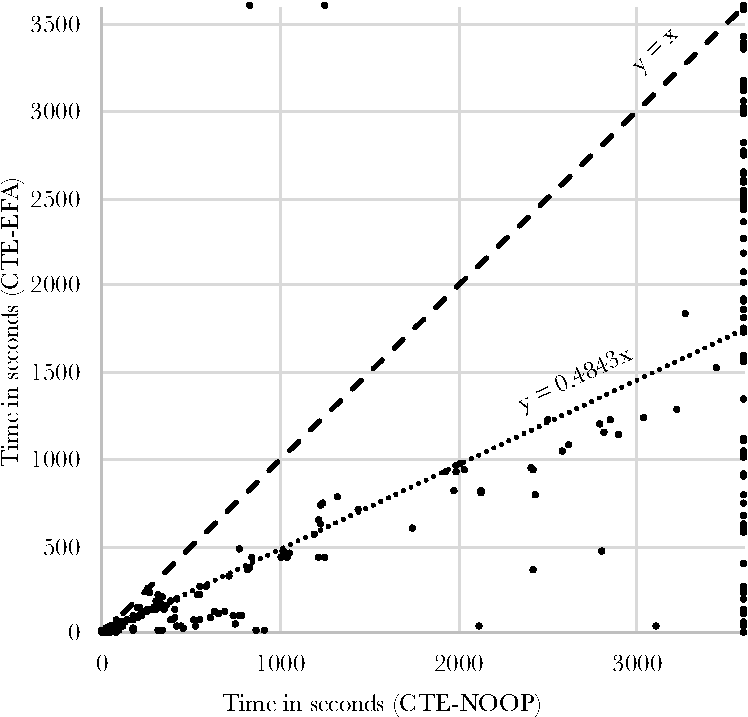
\includegraphics[width=.48\textwidth]{figures/time-plansat-efa-noop3} %\end{center}
\hfill
%\begin{center} 
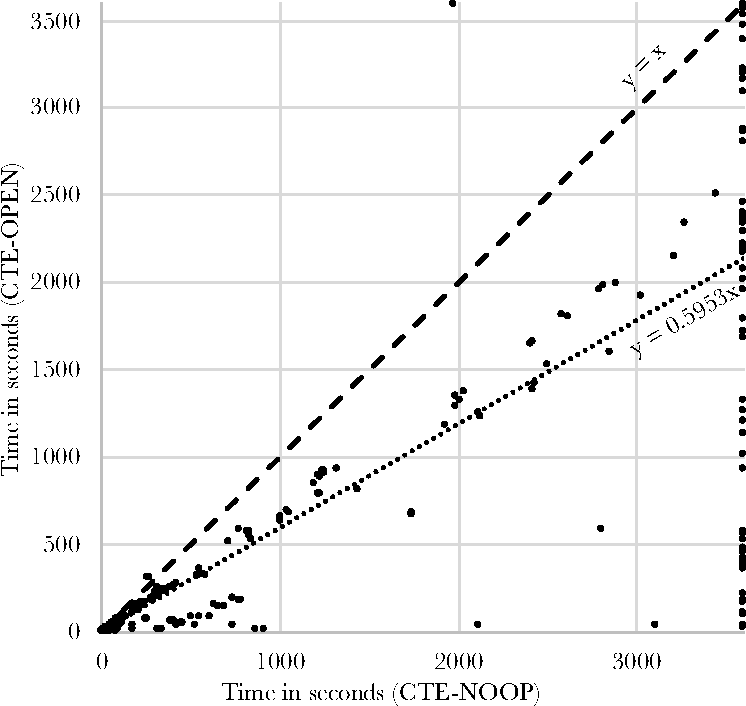
\includegraphics[width=.48\textwidth]{figures/time-plansat-open-noop3} \end{center}
\caption{Temps de décision (EFA/OPEN vs NOOP).}
\label{fig:plansat-noop}
\end{figure}

Nous avons testé la résolution de ces benchmarks avec nos nouveaux codages CTE-EFA et CTE-OPEN ainsi qu'avec le codage de l'état de l'art CTE-NOOP. Nous les avons comparés deux par deux en considérant le temps nécessaire pour prouver l'existence d'un plan (temps de décision, Figure~\ref{fig:plansat-noop}) et le temps global nécessaire pour obtenir un plan (temps d'extraction, Figure~\ref{fig:planextract-noop}). L'étape ``décision'' consiste à lancer de façon incrémentale le solveur QBF sur un CTE de profondeur croissante jusqu'à ce que le solveur retourne vrai ou atteigne la borne supérieure (nombre total de fluents). L'étape ``extraction'' consiste en un lancement du solveur par n\oe ud de l'arbre afin de récupérer le plan. Chaque test avait 60 minutes\footnote{L'étape d'instanciation des actions n'est pas incluse dans le temps écoulé.} de timeout pour la recherche du plan et 60 minutes pour son extraction.
Les résultats complets sont disponibles en ligne dans un fichier Excel\footnote{\url{https://www.irit.fr/~Frederic.Maris/documents/coplas2018/results.xls}}.

\begin{table*}
\centering
\begin{small}
\begin{tabular}{@{}lccccc@{}}
\toprule
Codage & Problèmes résolus & Temps de décision & Littéraux & Clauses & T/N \\ \midrule
CTE-NOOP & 412 sur 2112 (20\%) & 0\% & 0\% & 0\% & 30\% \\
CTE-EFA & 463 sur 2112 (22\%) & -55\% & -26\% & +15\% & 47\%  \\
CTE-OPEN & 445 sur 2112 (21\%) & -41\% & -2\% & -28\% & 17\% \\ \bottomrule
\\
\end{tabular}
\end{small}
\caption{Comparaison des codages présentés dans 65 domaines STRIPS des IPC 1 à 8 (sauf IPC 7) avec un total de 2112 problèmes. Le temps de décision, le nombre de littéraux, le nombre de clauses et le rapport transitions-sur-n\oe uds sont des moyennes. Transitions-sur-n\oe uds est le rapport moyen du nombre de contraintes basées sur des transitions divisé par le nombre de contraintes basées sur des n\oe uds (cf. Hypothèse 2, section Discussion ci-après).}
\label{fig:comparative}
\end{table*}

Les résultats montrent que nos codages CTE-EFA et CTE-OPEN sont plus efficaces que CTE-NOOP tant pour décider de l'existence d'un plan que pour l'extraire. CTE-EFA d'un facteur de 2,1 (1/0,4843) et CTE-OPEN d'un facteur de 1,7 (1/0,5953).  De plus, la comparaison entre CTE-EFA et CTE-OPEN (Figure~\ref{fig:plansat}, Figure~\ref{fig:planextract}) montre que CTE-EFA surpasse CTE-OPEN d'un facteur de 1,4 (1/0,7266). La Table~\ref{fig:comparative} donne un résumé des résultats sur les problèmes de référence.


% On IPC\_5/rovers/Propositional/Strips, the number of clauses and literals are very similar between NOOP and EFA. That said, EFA performs 46\% faster (in average).
% The correlation between the number of clauses and the performance gap between NOOP and EFA is not obvious. On average, NOOP encodings have 59\% more clauses than their EFA counterpart with the same number of literals
% OPEN encodings have the same number of clauses than NOOP but contain 20\% more literals.
%

Contrairement aux codages plats, le gain sur CTE-NOOP ne peut pas s'expliquer par une différence sur le nombre d'alternance des quantificateurs car la profondeur est la même dans les trois encodages. Cependant, la façon dont les actions sont représentées dans ces encodages pourrait expliquer cette différence.


\begin{figure}[ht!] \centering
\begin{center} 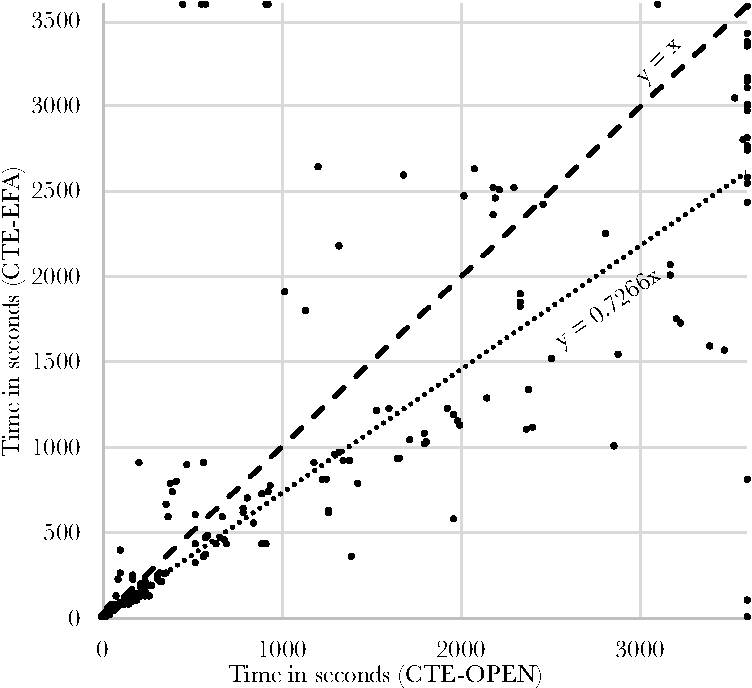
\includegraphics[width=.48\textwidth]{figures/time-plansat-efa-open3} \end{center}
\caption{Temps de décision (EFA vs OPEN).}
\label{fig:plansat}
\end{figure}

\begin{figure}[ht!] \centering
\begin{center} 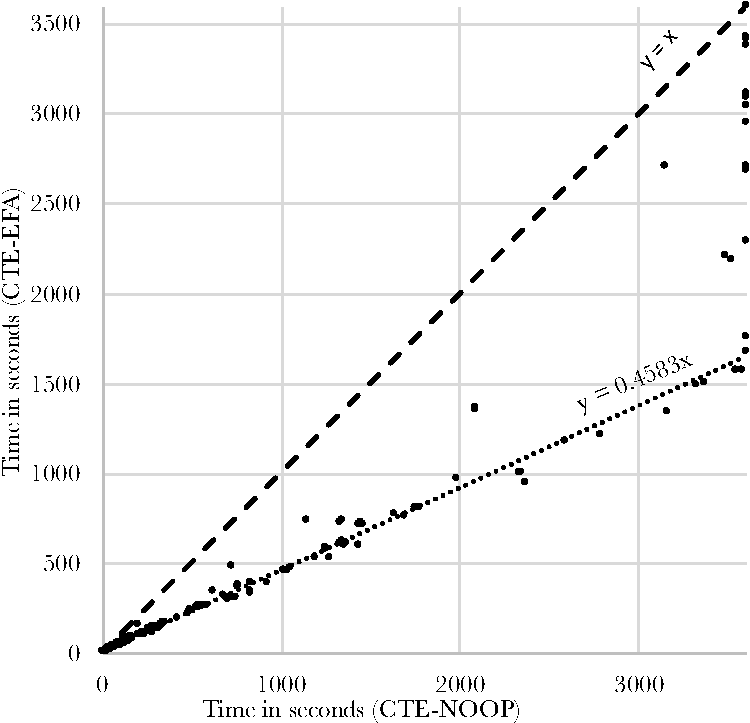
\includegraphics[width=.45\textwidth]{figures/time-extract-efa-noop3-good} %\end{center}
\hfill
%\begin{center} 
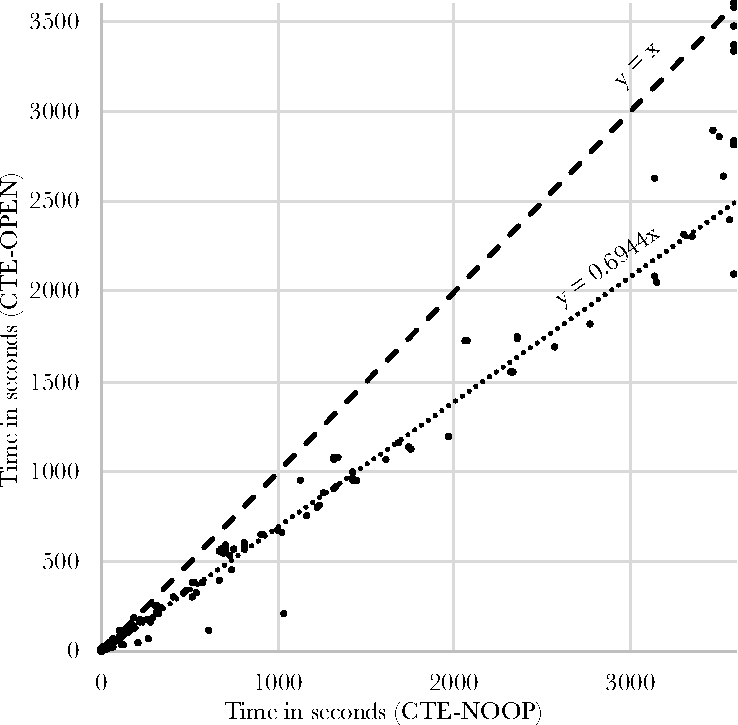
\includegraphics[width=.45\textwidth]{figures/time-extract-open-noop3} \end{center}
\caption{Temps d'extraction (EFA/OPEN vs NOOP).}
\label{fig:planextract-noop}
\end{figure}

\begin{figure}[ht!] \centering
\begin{center} 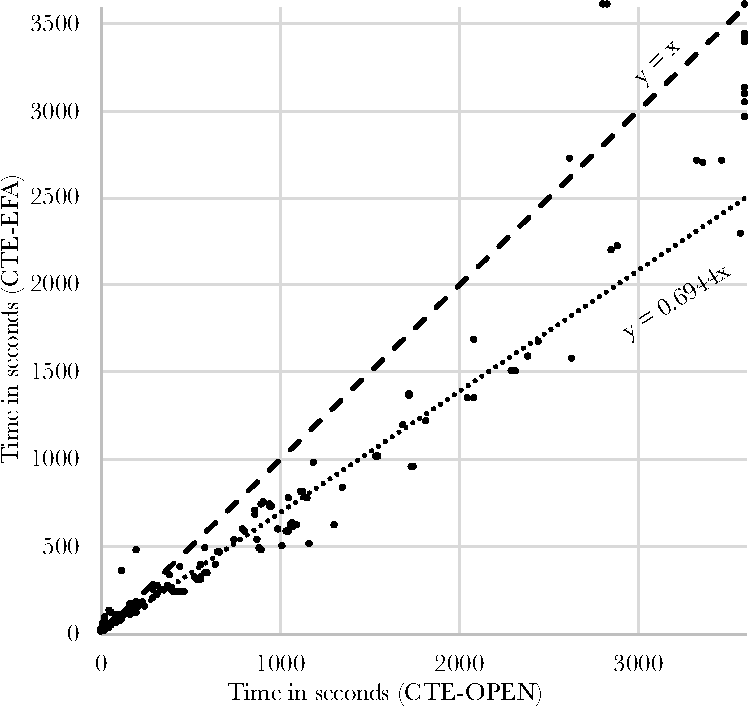
\includegraphics[width=.45\textwidth]{figures/time-extract-efa-open3-good} \end{center}
\caption{Temps d'extraction (EFA vs OPEN).}
\label{fig:planextract}
\end{figure}

\subsection{Discussion}

Pour tenter d'identifier les causes possibles de ces améliorations, nous avons proposé deux hypothèses, mises ensuite à l'épreuve avec nos tests:

\begin{description}
\item[Hypothèse 1] ``Le gain de performance est corrélé à une diminution du nombre de clauses et/ou de littéraux à travers les encodages''. Bien que la taille du problème soit notoirement non-corrélée à sa difficulté dans SAT, nous nous sommes demandés si nous pourrions voir la même non-corrélation. Comme le montre la Table~\ref{fig:comparative}, nous n'observons aucune tendance claire: CTE-EFA tend à avoir un nombre de clauses légèrement plus élevé (+15\%) que CTE-NOOP bien qu'il ait moins de variables (-26\%). CTE-OPEN a le même nombre de littéraux et beaucoup moins de clauses que CTE-NOOP, mais avec un gain de performances inférieur (-41\%) à CTE-EFA (-55\%). Cette non-corrélation nous a conduit à rejeter cette hypothèse.
~\\

\item[Hypothèse 2] ``Le gain de performance est dû à une différence dans le nombre de contraintes basées sur une transition par rapport au nombre de contraintes basées sur un n\oe ud''. Intuitivement, on peut penser qu'un ratio plus faible de contraintes basées sur les transitions sur les contraintes basées sur les n\oe uds faciliterait le processus de résolution: dans les contraintes basées sur les n\oe uds, une clause a le même contexte\footnote {Contexte et expansion sont définis dans \cite{DBLP:conf/ecai/CashmoreFG12}. Intuitivement, l'expansion est un arbre représentant la formule QBF et un contexte est une feuille dans cet arbre.} à travers l'extension QBF entière. Dans les contraintes de branche, la clause correspondante a des contextes différents selon la branche sélectionnée. L'idée est que les clauses basées sur différents contextes ralentissent le solveur. Comme le montre la Table~\ref{fig:comparative}, cette hypothèse ne semble pas pouvoir être étayée sur le plan expérimental: bien que CTE-OPEN montre un rapport transitions-sur-n\oe uds plus faible, il n'aboutit pas au meilleur gain de performance. Au contraire, le rapport CTE-EFA est plus faible, bien qu'il soit le plus efficace par rapport à CTE-NOOP. Nous avons donc aussi rejeté cette explication car nous n'avons noté aucune corrélation la soutenant, malgré une légère tendance où la diminution du temps et le nombre de clauses semblaient corrélées.
\end{description}

Aucune de nos deux hypothèses ne semblant donc être valable, la question de l'explication des gains de performance apportés par nos codages reste ouverte et sera l'objet de nos prochaines recherches.


\begin{figure}[ht!] \centering
\begin{center} 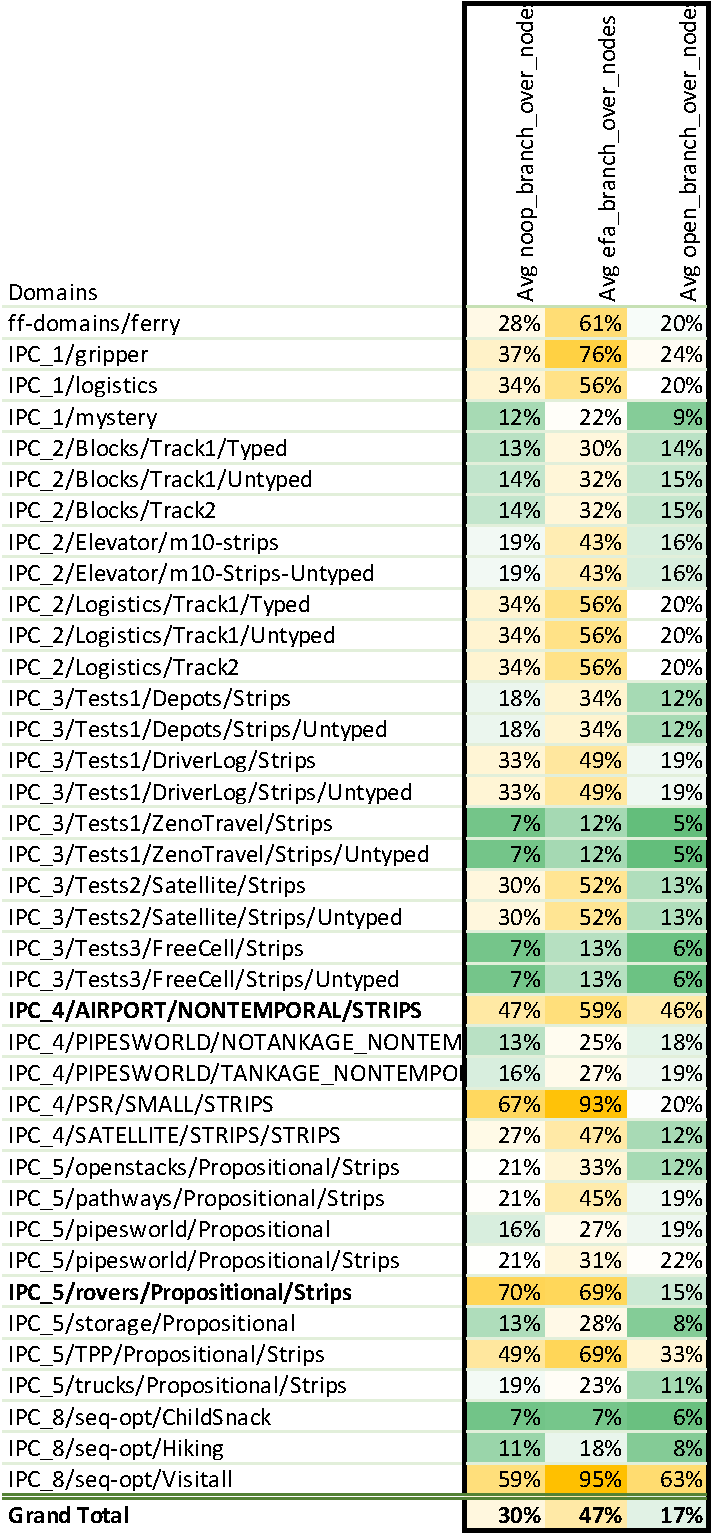
\includegraphics[width=.75\textwidth]{tableaux/experiment-branch_vs_nodes-crop.pdf} \end{center}
\caption{Rapport moyen B/N.}
\label{fig:tab-exp-branch-vs-nodes}
\end{figure}

\begin{figure}[ht!] \centering
\begin{center} 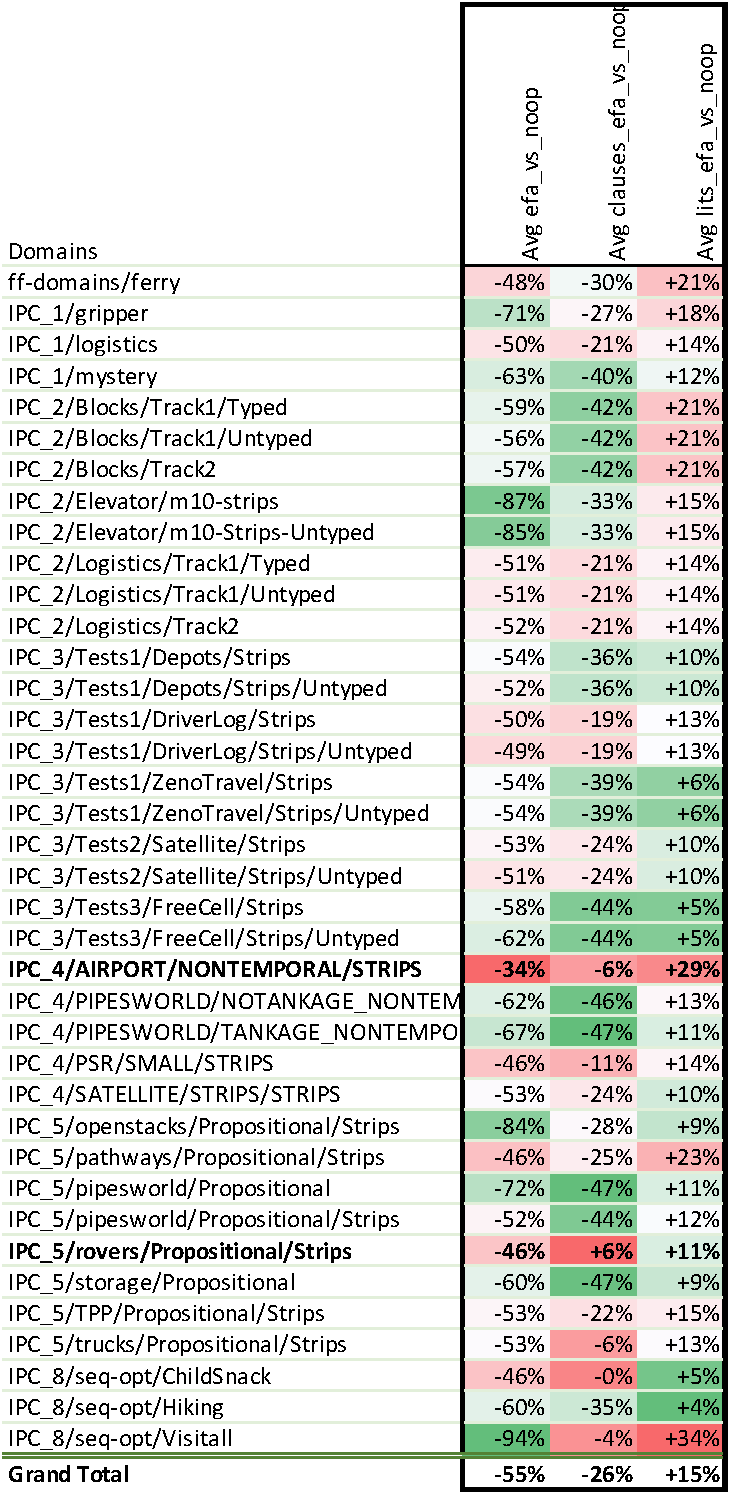
\includegraphics[width=.75\textwidth]{tableaux/experiment-efa_vs_noop-crop.pdf} \end{center}
\caption{Rapport moyen des performances CTE-EFA/CTE-NOOP.}
\label{fig:tab-exp-efa-vs-noop}
\end{figure}

\begin{figure}[ht!] \centering
\begin{center} 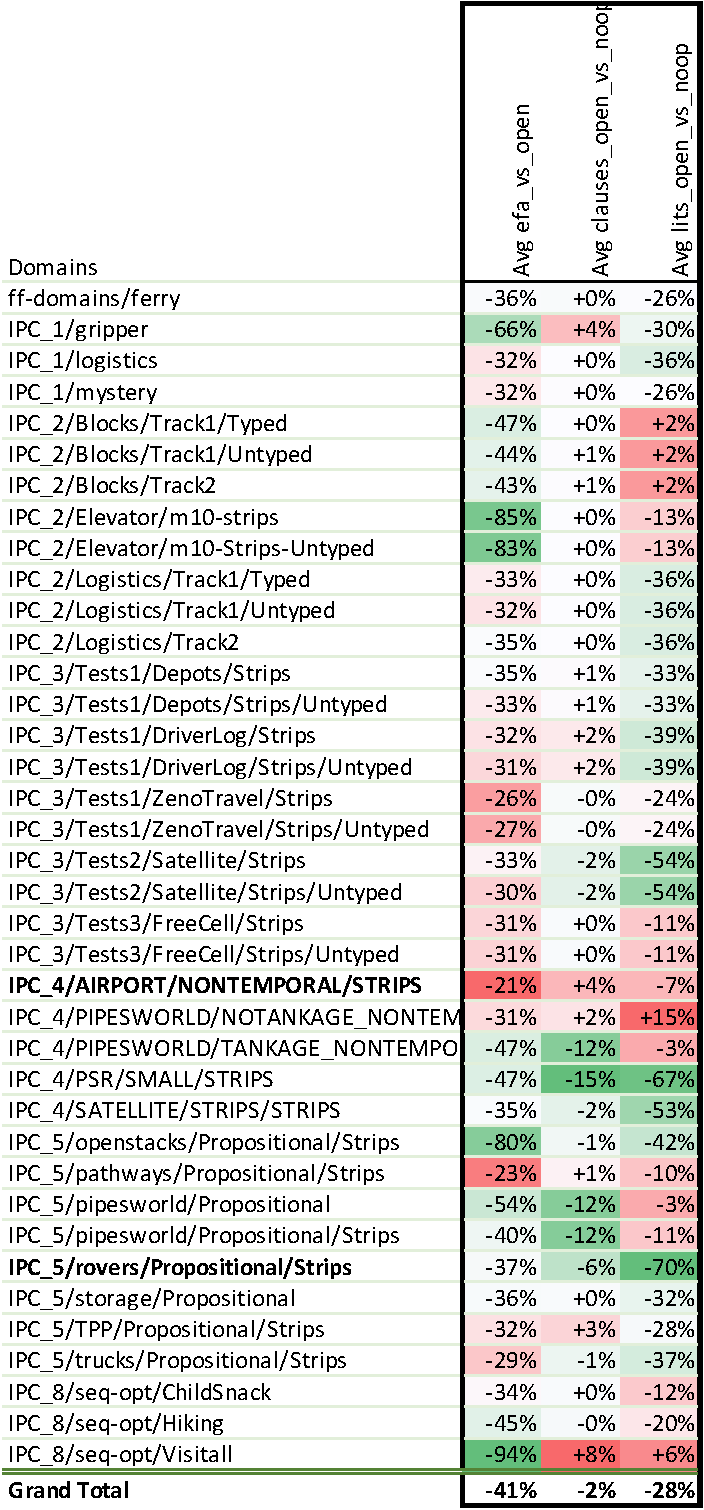
\includegraphics[width=.75\textwidth]{tableaux/experiment-efa_vs_open-crop.pdf} \end{center}
\caption{Rapport moyen des performances CTE-EFA/CTE-OPEN.}
\label{fig:tab-exp-efa-vs-open}
\end{figure}

%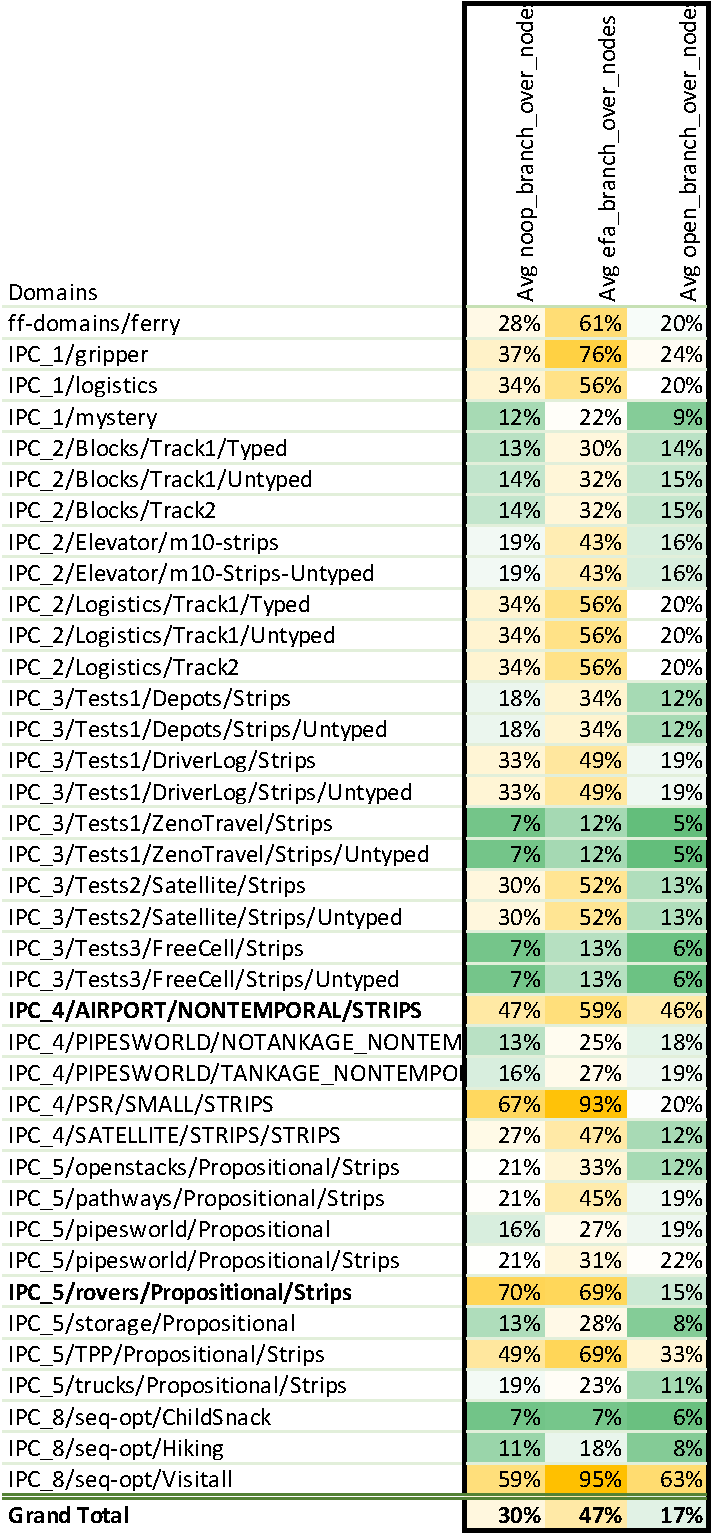
\includegraphics[width=0.5\textwidth]{tableaux/experiment-branch_vs_nodes-crop.pdf}

%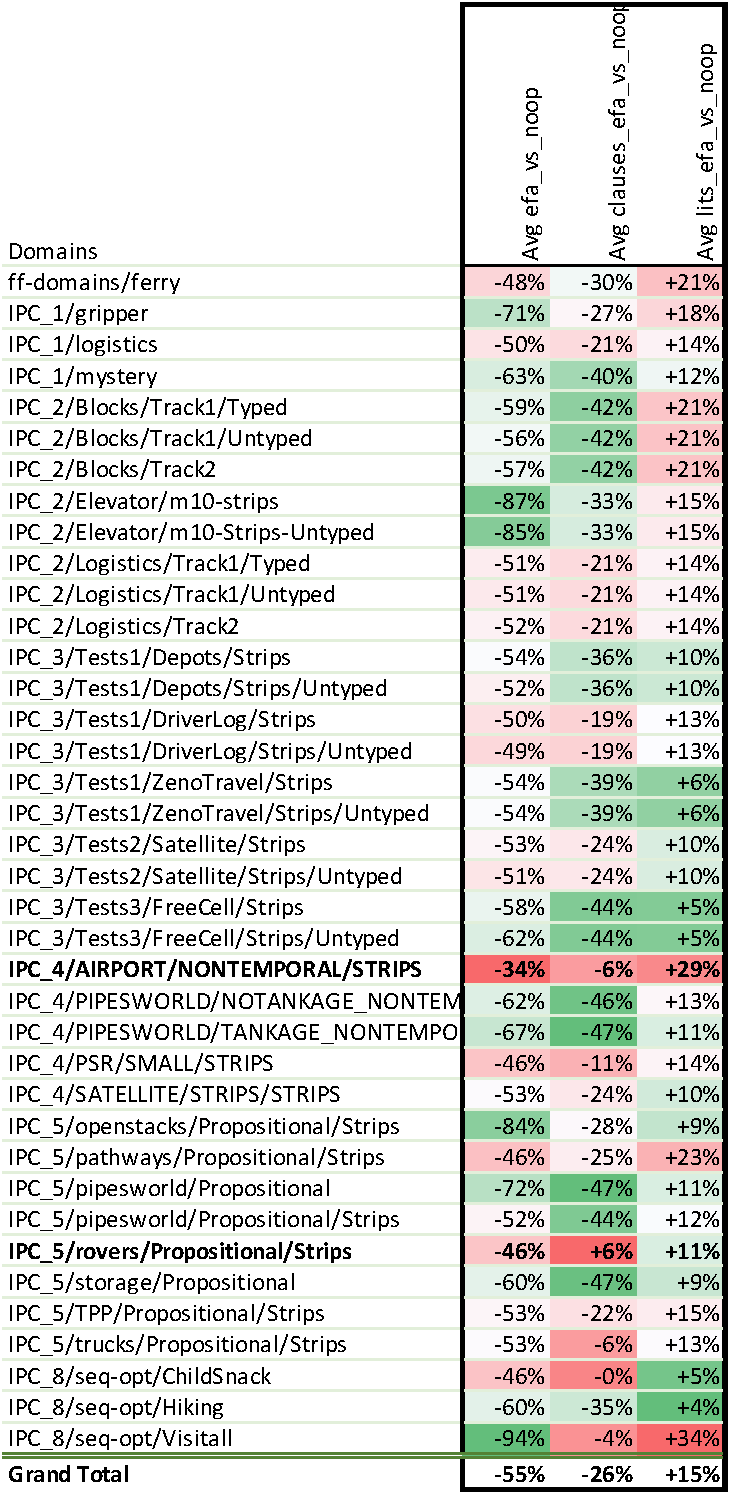
\includegraphics[scale=0.95]{tableaux/experiment-efa_vs_noop-crop.pdf}

%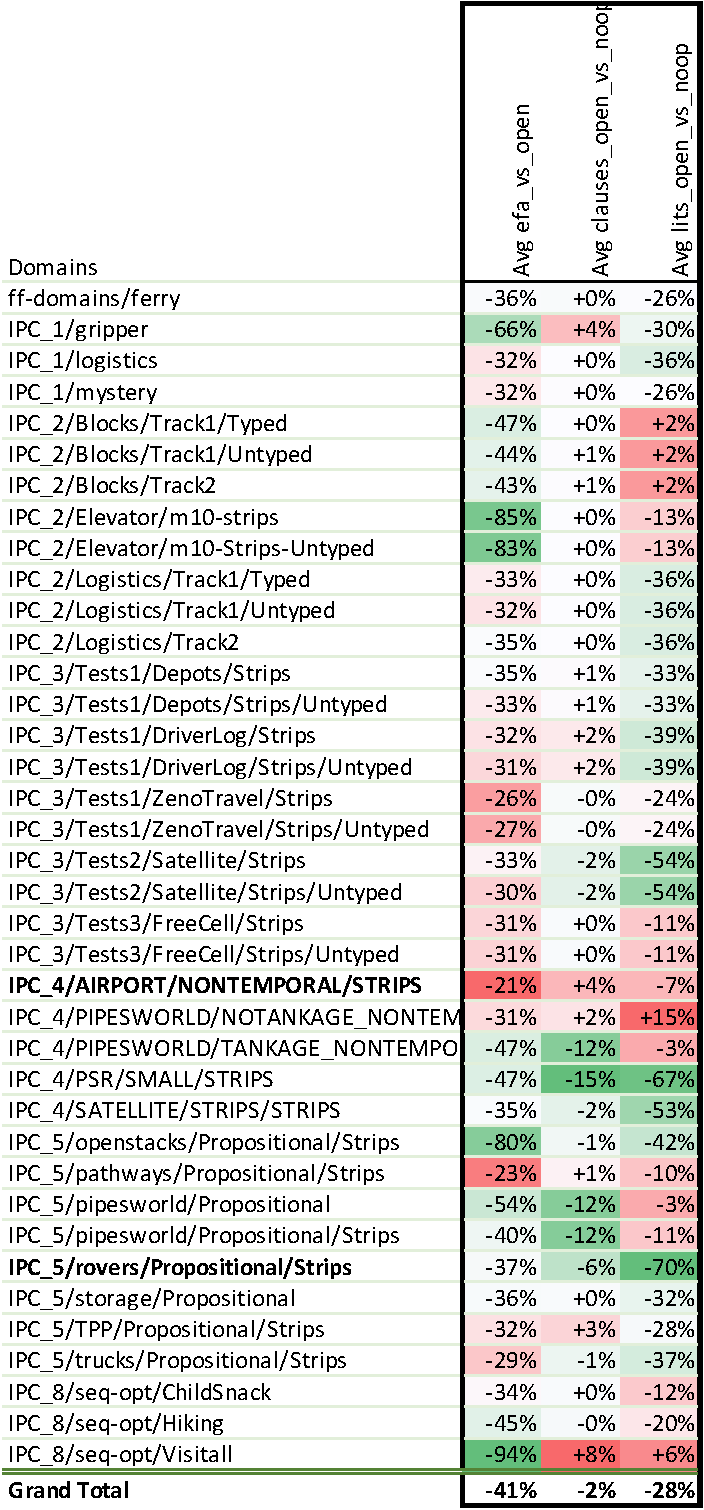
\includegraphics{tableaux/experiment-efa_vs_open-crop.pdf}


%%%%%%%%%%%%%%%%%%%%%%%%%%%%%%%%%%%%%%%%%%%%%%%%%%%%%%%%%%%%
% TESTS : PLANIFICATION SMT
%%%%%%%%%%%%%%%%%%%%%%%%%%%%%
%\subsection{Planification temporelle avec SMT}


%\subsection{Jeux avec QBF}


%%%%%%%%%%%%%%%%%%%%%
% CONCLUSION
%%%%%%%%%%%%%%%%%%%%%

\chapter{Conclusion et perspectives}
\section{Ce que nous avons réalisé}

Dans cette thèse, nous avons présenté \touist, un outil de traduction automatique de problèmes en formules logique que nous avons développé. Cet outil permet d'utiliser facilement différents solveurs SAT, SMT ou QBF puisqu'il effectue lui même lorsque nécessaire, une mise en forme prénexe ou en forme normale conjonctive en utilisant la transformation de Tseitin avant de traduire la formule au format DIMACS, QDIMACS ou SMT-LIB en fonction du solveur externe utilisé. Il permet en retour, d'afficher les résultats renvoyés par le solveur dans un format directement lisible par l'utilisateur, en rapport avec les noms de variables définies par ce dernier.

Nous avons montré comment utiliser le langage de \touist pour exprimer de manière simple des problèmes combinatoires statiques avec SAT, comme le Sudoku. Nous avons aussi montré qu'il est possible de coder aussi facilement des problèmes dynamiques, comme le jeu de Nim, pour lesquel l'utilisation d'un codage QBF nous permet de calculer un stratégie gagnante. Nous avons également montré comment utiliser SMT pour obtenir, grâce à des contraintes d'arithmétique linéaire, un codage plus compact et plus facile à exprimer pour le Takuzu.

Afin d'utiliser \touist pour compiler des problèmes de planification en logique pour les résoudre, nous avons développé le module \touistplan qui intègre différentes méthodes de codage.
Nous avons notamment proposé un nouveau codage SAT et deux nouveaux codages d'arbres compacts QBF pour la planification classique, ainsi qu'un nouveau codage SMT pour la planification temporelle en temps continu. Nous avons montré, par une étude expérimentale sur les benchmarks des compétitions IPC en utilisant \touistplan avec différents solveurs QBF, que nos nouveaux codages QBF sont en moyenne deux fois plus efficaces que le codage de l'état de l'art.

\section{Ce qu'il reste à explorer}

D'une part, de nombreuses perspectives sont ouvertes concernant l'extension de notre traducteur \touist, tant du point de vue des langages d'entrée et des modules de traduction automatique intégrés, que de des langages de sortie et des solveurs utilisés.

L'une des perspectives immédiates serait d'implémenter de nouveaux modules d'entrée pour permettre d'utiliser \touist avec des langages spécifiques, comme nous l'avons fait pour le langage PDDL avec \touistplan.
Nous avons notamment travaillé à l'extension du langage de \touist à DL-PA (Dynamic Logic of Propositional Assignments)~\cite{DBLP:conf/lics/BalbianiHT13} en intégrant une traduction des formules DL-PA vers QBF proposée par Andreas Herzig et Abdallah Saffidine. En l'implémentant nous avons eu des premiers résultats intéressants. Notre objectif est de pouvoir fournir, à terme, un prouveur automatique pour DL-PA.

Une autre voie d'extension de \touist serait d'augmenter le langage d'entrée de \touist pour prendre en compte des atomes d'autres théories que QF-IDL, QF-RDL, QF-LIA ou QF-LRA. Ceci permettrait de l'interfacer avec des solveurs SMT prenant en charge ces nouvelles théories.

Enfin, un travail exploratoire a été commencé sur l'interfaçage entre \touist et l'interface de production de sémantiques argumentatives SESAME (\url{https://www.irit.fr/SESAME/}). Celle-ci, développée au sein de l'équipe LILaC, permet de produire de manière interactive des sémantiques argumentatives dans un langage du premier ordre et domaine fini. L'idée serait de fournir à \touist :
\begin{itemize}
    \item une sémantique argumentative,
    \item un arbre argumentatif dont les sommets sont des arguments et les liens entre ces sommets une relation d'attaque entre arguments,
    \item et un ensemble d'arguments
\end{itemize}
afin que \touist détermine si, en fonction de la sémantique et de l'arbre argumentatif, cet ensemble d'argument constitue une extension possible de la sémantique.\\


D'autre part, nous avons également ouvert des perspectives pour augmenter encore les performances de la planification par compilation.

Dans la cadre de la planification classique, nous avons montré que pour l'approche QBF, au-delà des améliorations sur les solveurs, d'autres travaux doivent être menés pour mettre au point des codages plus performants. Comme nous l'avons indiqué, cela a déjà été réalisé pour SAT avec des améliorations significatives.

Dans le cadre de la planification temporelle en temps continu, le codage SMT que nous avons proposé, bien que plus compact que le codage de référence existant, doit encore être amélioré pour permettre une meilleure efficacité en terme de temps de résolution des problèmes.

%Nous présentons ici deux nouveaux codages d'arbres compacts CTE (Compact Tree Encoding) de problèmes de planification en QBF: CTE-EFA basé sur des frame-axiomes explicatifs dans un espace d'états, et CTE-OPEN basé sur des liens de causalité dans un espace de plans. \fred{dans le chapitre EXPERIMENTATIONS:} Nous les comparons au codage de l'état de l'art CTE-NOOP basé sur des actions No-op et proposé dans \cite{DBLP:conf/ecai/CashmoreFG12}. En termes de temps d'exécution par rapport aux problèmes de référence, CTE-EFA et CTE-OPEN sont toujours plus efficaces que CTE-NOOP.

\appendix
\chapter{Annexes}
\section{Grammaire BNF du langage \touist}
%\renewcommand{\textless}[1]{\bf$\langle$}
%\renewcommand{\textgreater}[1]{$\rangle$}
%\renewcommand{\mdcolor}[1]{}

\noindent Nous présentons ici la grammaire de TouIST sous forme BNF. Certaines règles (une règle commence avec "\mdcode{::=}\textquotedblleft{}) sont paramétrées de telle sorte que des parties de la grammaire soient factorisées (l'idée de règles paramétrées provient du parser \emph{Menhir} que nous avons utilisé pour développer le parser de \touist.%mdk

\noindent\textbf{Remarque}.
Cette grammaire n'est pas LR(1) et ne peut être implémentée telle quelle en utilisant \emph{Menhir} ; une large part de la vérification de type est réalisée après la production de l'arbre de syntaxe abstraite. L'objectif de cette spécification est de présenter de la manière la plus claire et la plus synthétique possible ce que le langage de \touist permet ou non d'exprimer.%mdk%mdk

\begin{footnotesize}

\begin{mdpre}%mdk
\noindent INT~~~~~~~=~{}[0-9]+\\
FLOAT~~~~~=~{}[0-9]+\textbackslash{}.{}[0-9]+\\
TERM~~~~~~=~{}[\_0-9]*{}[a-zA-Z]{}[a-zA-Z\_0-9]*%mdk
\end{mdpre}\begin{mdpre}%mdk
\noindent{\mdcolor{purple}\textless{}touist-file\textgreater{}}~::=~{\mdcolor{purple}\textless{}assign\textgreater{}}~{\mdcolor{purple}\textless{}touist-file\textgreater{}}\\
~~~~~~~~~~~~~~~~~\textbar{}~{\mdcolor{purple}\textless{}formula\textgreater{}}~{\mdcolor{purple}\textless{}touist-file\textgreater{}}\\
~~~~~~~~~~~~~~~~~\textbar{}~EOF\\
\\
{\mdcolor{purple}\textless{}expr\textgreater{}}~::=~{\mdcolor{purple}\textless{}int\textgreater{}}\textbar{}{\mdcolor{purple}\textless{}float\textgreater{}}\textbar{}{\mdcolor{purple}\textless{}prop\textgreater{}}\textbar{}{\mdcolor{purple}\textless{}bool\textgreater{}}\textbar{}{\mdcolor{purple}\textless{}set\textgreater{}}\\
~~~~\textbar{}~"""{\mdcolor{purple}\textless{}formula-simple\textgreater{}}"""~~{\mdcolor{darkgreen}\textless{}-~Touist~\textgreater{}=~3.5.1}\\
{\mdcolor{purple}\textless{}var\textgreater{}}~::=~"\$"~TERM\\
~~~~\textbar{}~"\$"~TERM~"("~{\mdcolor{purple}\textless{}comma-list(\textless{}expr\textgreater{})\textgreater{}}~")"\\
\\
{\mdcolor{purple}\textless{}prop\textgreater{}}~::=\\
~~~~\textbar{}~{\mdcolor{purple}\textless{}var\textgreater{}}\\
~~~~\textbar{}~TERM\\
~~~~\textbar{}~TERM~"("~{\mdcolor{purple}\textless{}comma-list(\textless{}expr\textgreater{})\textgreater{}}~")"\\
\\
{\mdcolor{purple}\textless{}assign\textgreater{}}~::=~{\mdcolor{purple}\textless{}var\textgreater{}}~"="~({\mdcolor{purple}\textless{}expr\textgreater{}})\\
\\
{\mdcolor{purple}\textless{}let-assign\textless{}T\textgreater{}\textgreater{}}~::=\\
~~~~\textbar{}~"let"~{\mdcolor{purple}\textless{}var\textgreater{}}~"="~{\mdcolor{purple}\textless{}expr\textgreater{}}~":"~{\mdcolor{purple}\textless{}formula\textless{}T\textgreater{}\textgreater{}}\\
~~~~\textbar{}~"let"~{\mdcolor{purple}\textless{}comma-list(\textless{}var\textgreater{})\textgreater{}}~"="~{\mdcolor{purple}\textless{}comma-list(\textless{}expr\textgreater{})\textgreater{}}\\
~~~~~~~~~~~~~~~~~~~~~~~~~~~~~":"~{\mdcolor{purple}\textless{}formula\textless{}T\textgreater{}\textgreater{}}\\
\\
{\mdcolor{purple}\textless{}equality(\textless{}T\textgreater{})\textgreater{}}~::=\\
~~~~\textbar{}~{\mdcolor{purple}\textless{}T\textgreater{}}~"!="~{\mdcolor{purple}\textless{}T\textgreater{}}\\
~~~~\textbar{}~{\mdcolor{purple}\textless{}T\textgreater{}}~"=="~{\mdcolor{purple}\textless{}T\textgreater{}}\\
\\
{\mdcolor{purple}\textless{}order(\textless{}T\textgreater{})\textgreater{}}~::=\\
~~~~\textbar{}~{\mdcolor{purple}\textless{}T\textgreater{}}~"\textgreater{}"~{\mdcolor{purple}\textless{}T\textgreater{}}\\
~~~~\textbar{}~{\mdcolor{purple}\textless{}T\textgreater{}}~"\textless{}"~{\mdcolor{purple}\textless{}T\textgreater{}}\\
~~~~\textbar{}~{\mdcolor{purple}\textless{}T\textgreater{}}~"\textless{}="~{\mdcolor{purple}\textless{}T\textgreater{}}\\
~~~~\textbar{}~{\mdcolor{purple}\textless{}T\textgreater{}}~"\textgreater{}="~{\mdcolor{purple}\textless{}T\textgreater{}}\\
\\
{\mdcolor{purple}\textless{}bool\textgreater{}}~::=~"("~{\mdcolor{purple}\textless{}bool\textgreater{}}~")"\\
~~~~\textbar{}~{\mdcolor{purple}\textless{}var\textgreater{}}\\
~~~~\textbar{}~"true"\\
~~~~\textbar{}~"false"\\
~~~~\textbar{}~({\mdcolor{purple}\textless{}expr\textgreater{}})~"in"~{\mdcolor{purple}\textless{}set\textgreater{}}\\
~~~~\textbar{}~"subset("~{\mdcolor{purple}\textless{}set\textgreater{}}~","~{\mdcolor{purple}\textless{}set\textgreater{}}~")"\\
~~~~\textbar{}~"empty("~{\mdcolor{purple}\textless{}set\textgreater{}}~")"\\
~~~~\textbar{}~{\mdcolor{purple}\textless{}equality(\textless{}int\textgreater{}}\textbar{}{\mdcolor{purple}\textless{}float\textgreater{}}\textbar{}{\mdcolor{purple}\textless{}prop\textgreater{})\textgreater{}}\\
~~~~\textbar{}~{\mdcolor{purple}\textless{}order(\textless{}int\textgreater{}}\textbar{}{\mdcolor{purple}\textless{}float\textgreater{})\textgreater{}}\\
~~~~\textbar{}~{\mdcolor{purple}\textless{}connectors(\textless{}bool\textgreater{})\textgreater{}}\\
\\
{\mdcolor{purple}\textless{}num-operation(\textless{}T\textgreater{})\textgreater{}}~::=\\
~~~~\textbar{}~{\mdcolor{purple}\textless{}T\textgreater{}}~"+"~{\mdcolor{purple}\textless{}T\textgreater{}}\\
~~~~\textbar{}~{\mdcolor{purple}\textless{}T\textgreater{}}~"-"~{\mdcolor{purple}\textless{}T\textgreater{}}\\
~~~~\textbar{}~~~~~"-"~{\mdcolor{purple}\textless{}T\textgreater{}}\\
~~~~\textbar{}~{\mdcolor{purple}\textless{}T\textgreater{}}~"*"~{\mdcolor{purple}\textless{}T\textgreater{}}\\
~~~~\textbar{}~{\mdcolor{purple}\textless{}T\textgreater{}}~"/"~{\mdcolor{purple}\textless{}T\textgreater{}}\\
\\
{\mdcolor{purple}\textless{}num-operation-others(\textless{}T\textgreater{})\textgreater{}}~::=\\
~~~~\textbar{}~{\mdcolor{purple}\textless{}T\textgreater{}}~"mod"~{\mdcolor{purple}\textless{}T\textgreater{}}\\
~~~~\textbar{}~"abs("~{\mdcolor{purple}\textless{}T\textgreater{}}~")"\\
\\
{\mdcolor{purple}\textless{}int\textgreater{}}~::=\\
~~~~\textbar{}~"("~{\mdcolor{purple}\textless{}int\textgreater{}}~")"\\
~~~~\textbar{}~{\mdcolor{purple}\textless{}var\textgreater{}}\\
~~~~\textbar{}~INT\\
~~~~\textbar{}~num-operation({\mdcolor{purple}\textless{}int\textgreater{}})\\
~~~~\textbar{}~num-operation-others({\mdcolor{purple}\textless{}int\textgreater{}})\\
~~~~\textbar{}~"if"~{\mdcolor{purple}\textless{}bool\textgreater{}}~"then"~{\mdcolor{purple}\textless{}int\textgreater{}}~"else"~{\mdcolor{purple}\textless{}int\textgreater{}}~"end"\\
~~~~\textbar{}~"int("~({\mdcolor{purple}\textless{}int\textgreater{}}\textbar{}{\mdcolor{purple}\textless{}float\textgreater{}})~")"\\
~~~~\textbar{}~"card("~{\mdcolor{purple}\textless{}set\textgreater{}}~")"\\
\\
{\mdcolor{purple}\textless{}float\textgreater{}}~::=\\
~~~~\textbar{}~"("~{\mdcolor{purple}\textless{}float\textgreater{}}~")"\\
~~~~\textbar{}~{\mdcolor{purple}\textless{}var\textgreater{}}\\
~~~~\textbar{}~FLOAT\\
~~~~\textbar{}~num-operation({\mdcolor{purple}\textless{}float\textgreater{}})\\
~~~~\textbar{}~num-operation-others({\mdcolor{purple}\textless{}float\textgreater{}})\\
~~~~\textbar{}~"if"~{\mdcolor{purple}\textless{}bool\textgreater{}}~"then"~{\mdcolor{purple}\textless{}float\textgreater{}}~"else"~{\mdcolor{purple}\textless{}float\textgreater{}}~"end"\\
~~~~\textbar{}~"float("~({\mdcolor{purple}\textless{}int\textgreater{}}\textbar{}{\mdcolor{purple}\textless{}float\textgreater{}})~~")"\\
~~~~\textbar{}~"sqrt("~{\mdcolor{purple}\textless{}float\textgreater{}}~")"\\
\\
{\mdcolor{purple}\textless{}set\textgreater{}}~::=~"("~{\mdcolor{purple}\textless{}set\textgreater{}}~")"\\
~~~~\textbar{}~{\mdcolor{purple}\textless{}var\textgreater{}}\\
~~~~\textbar{}~"{}["~{\mdcolor{purple}\textless{}comma-list(\textless{}expr\textgreater{})\textgreater{}}~"]"\\
~~~~\textbar{}~"{}[~{\mdcolor{purple}\textless{}int\textgreater{}}~".."~{\mdcolor{purple}\textless{}int\textgreater{}}~"]"~~~~~~{\mdcolor{darkgreen}\textless{}-~step~is~1}\\
~~~~\textbar{}~"{}[~{\mdcolor{purple}\textless{}float\textgreater{}}~".."~{\mdcolor{purple}\textless{}float\textgreater{}}~"]"~~{\mdcolor{darkgreen}\textless{}-~step~is~1.0}\\
~~~~\textbar{}~"{}[~{\mdcolor{purple}\textless{}expr\textgreater{}}~"for"~{\mdcolor{purple}\textless{}comma-list(\textless{}var\textgreater{})\textgreater{}}\\
~~~~~~~"in"~{\mdcolor{purple}\textless{}comma-list(\textless{}set\textgreater{})\textgreater{}}~{}["when"~{\mdcolor{purple}\textless{}bool\textgreater{}}]~"]"~~{\mdcolor{darkgreen}\textless{}-~TouIST~\textgreater{}=~3.5.2}\\
~~~~\textbar{}~{\mdcolor{purple}\textless{}set\textgreater{}}~"inter"~{\mdcolor{purple}\textless{}set\textgreater{}}~~~~~~~~~~{\mdcolor{darkgreen}\textless{}-~TouIST~\textgreater{}=~3.4.0}\\
~~~~\textbar{}~{\mdcolor{purple}\textless{}set\textgreater{}}~"union"~{\mdcolor{purple}\textless{}set\textgreater{}}~~~~~~~~~~{\mdcolor{darkgreen}\textless{}-~TouIST~\textgreater{}=~3.4.0}\\
~~~~\textbar{}~{\mdcolor{purple}\textless{}set\textgreater{}}~"diff"~{\mdcolor{purple}\textless{}set\textgreater{}}~~~~~~~~~~~{\mdcolor{darkgreen}\textless{}-~TouIST~\textgreater{}=~3.4.0}\\
~~~~\textbar{}~"union("~{\mdcolor{purple}\textless{}set\textgreater{}}~","~{\mdcolor{purple}\textless{}set\textgreater{}}~")"\\
~~~~\textbar{}~"inter("~{\mdcolor{purple}\textless{}set\textgreater{}}~","~{\mdcolor{purple}\textless{}set\textgreater{}}~")"\\
~~~~\textbar{}~"diff("~{\mdcolor{purple}\textless{}set\textgreater{}}~","~{\mdcolor{purple}\textless{}set\textgreater{}}~")"\\
~~~~\textbar{}~"powerset("~{\mdcolor{purple}\textless{}set\textgreater{}}~")"\\
\\
{\mdcolor{purple}\textless{}comma-list(\textless{}T\textgreater{})\textgreater{}}~::=~{\mdcolor{purple}\textless{}T\textgreater{}}~\textbar{}~{\mdcolor{purple}\textless{}T\textgreater{}}~","~{\mdcolor{purple}\textless{}comma-list(\textless{}T\textgreater{})\textgreater{}}\\
\\
{\mdcolor{purple}\textless{}generalized-connectors(\textless{}T\textgreater{})\textgreater{}}~::=\\
~~~~\textbar{}~"bigand"~{\mdcolor{purple}\textless{}comma-list(\textless{}var\textgreater{})\textgreater{}}~"in"~{\mdcolor{purple}\textless{}comma-list(\textless{}set\textgreater{})\textgreater{}}\\
~~~~~~~~~~~~~~~~~~~~~~~~~~~~~{}["when"~{\mdcolor{purple}\textless{}bool\textgreater{}}]~":"~{\mdcolor{purple}\textless{}T\textgreater{}}~"end"\\
~~~~\textbar{}~"bigor"~{\mdcolor{purple}\textless{}comma-list(\textless{}var\textgreater{})\textgreater{}}~"in"~{\mdcolor{purple}\textless{}comma-list(\textless{}set\textgreater{})\textgreater{}}\\
~~~~~~~~~~~~~~~~~~~~~~~~~~~~~{}["when"~{\mdcolor{purple}\textless{}bool\textgreater{}}]~":"~{\mdcolor{purple}\textless{}T\textgreater{}}~"end"\\
~~~~\textbar{}~"exact("~{\mdcolor{purple}\textless{}int\textgreater{}}~","~{\mdcolor{purple}\textless{}set\textgreater{}}~")"\\
~~~~\textbar{}~"atmost("~{\mdcolor{purple}\textless{}int\textgreater{}}~","~{\mdcolor{purple}\textless{}set\textgreater{}}~")"\\
~~~~\textbar{}~"atleast("~{\mdcolor{purple}\textless{}int\textgreater{}}~","~{\mdcolor{purple}\textless{}set\textgreater{}}~")"\\
\\
{\mdcolor{purple}\textless{}connectors(\textless{}T\textgreater{})\textgreater{}}~::=\\
~~~~\textbar{}~~~~~"not"~{\mdcolor{purple}\textless{}T\textgreater{}}\\
~~~~\textbar{}~{\mdcolor{purple}\textless{}T\textgreater{}}~"and"~{\mdcolor{purple}\textless{}T\textgreater{}}\\
~~~~\textbar{}~{\mdcolor{purple}\textless{}T\textgreater{}}~"or"~{\mdcolor{purple}\textless{}T\textgreater{}}\\
~~~~\textbar{}~{\mdcolor{purple}\textless{}T\textgreater{}}~"xor"~{\mdcolor{purple}\textless{}T\textgreater{}}\\
~~~~\textbar{}~{\mdcolor{purple}\textless{}T\textgreater{}}~"=\textgreater{}"~{\mdcolor{purple}\textless{}T\textgreater{}}\\
~~~~\textbar{}~{\mdcolor{purple}\textless{}T\textgreater{}}~"\textless{}=\textgreater{}"~{\mdcolor{purple}\textless{}T\textgreater{}}\\
\\
{\mdcolor{purple}\textless{}formula(\textless{}T\textgreater{})\textgreater{}}~::=\\
~~~~\textbar{}~"\textbackslash{}\textbackslash{}"~{\mdcolor{purple}\textless{}T\textgreater{}}~\textbar{}~{\mdcolor{purple}\textless{}T\textgreater{}}~"\textbackslash{}\textbackslash{}"~~~~~~~~~~~~~{\mdcolor{darkgreen}\textless{}-~newline~marker~for~latex~display}\\
~~~~\textbar{}~"("~{\mdcolor{purple}\textless{}T\textgreater{}}~")"\\
~~~~\textbar{}~"if"~{\mdcolor{purple}\textless{}bool\textgreater{}}~"then"~{\mdcolor{purple}\textless{}T\textgreater{}}~"else"~{\mdcolor{purple}\textless{}T\textgreater{}}~"end"\\
~~~~\textbar{}~{\mdcolor{purple}\textless{}connectors(\textless{}T\textgreater{})\textgreater{}}\\
~~~~\textbar{}~{\mdcolor{purple}\textless{}generalized-connectors(\textless{}T\textgreater{})\textgreater{}}\\
~~~~\textbar{}~{\mdcolor{purple}\textless{}let-assign(\textless{}T\textgreater{})\textgreater{}}\\
~~~~\textbar{}~{\mdcolor{purple}\textless{}T\textgreater{}}~("\textbackslash{}n"\textbar{}"~")~{\mdcolor{purple}\textless{}T\textgreater{}}~~~{\mdcolor{darkgreen}\textless{}-~newline/whitespace~in~top-level~is~an~'and'}\\
\\
{\mdcolor{purple}\textless{}formula-simple\textgreater{}}~::=\\
~~~~\textbar{}~"Top"\\
~~~~\textbar{}~"Bot"\\
~~~~\textbar{}~{\mdcolor{purple}\textless{}prop\textgreater{}}\\
~~~~\textbar{}~{\mdcolor{purple}\textless{}var\textgreater{}}\\
~~~~\textbar{}~{\mdcolor{purple}\textless{}formula(\textless{}formula-simple\textgreater{})\textgreater{}}\\
\\
{\mdcolor{purple}\textless{}formula-smt\textgreater{}}~::=\\
~~~~\textbar{}~{\mdcolor{purple}\textless{}formula(\textless{}formula-smt\textgreater{})\textgreater{}}\\
~~~~\textbar{}~{\mdcolor{purple}\textless{}expr-smt\textgreater{}}\\
\\
{\mdcolor{purple}\textless{}expr-smt\textgreater{}}~::=\\
~~~~\textbar{}~"Top"\\
~~~~\textbar{}~"Bot"\\
~~~~\textbar{}~{\mdcolor{purple}\textless{}prop\textgreater{}}\\
~~~~\textbar{}~{\mdcolor{purple}\textless{}var\textgreater{}}\\
~~~~\textbar{}~{\mdcolor{purple}\textless{}int\textgreater{}}\\
~~~~\textbar{}~{\mdcolor{purple}\textless{}float\textgreater{}}\\
~~~~\textbar{}~{\mdcolor{purple}\textless{}order\textgreater{}(\textless{}expr-smt\textgreater{}})\\
~~~~\textbar{}~\textless{}num-operations\_standard({\mdcolor{purple}\textless{}expr-smt\textgreater{})\textgreater{}}\\
~~~~\textbar{}~{\mdcolor{purple}\textless{}equality(\textless{}expr-smt\textgreater{})\textgreater{}}\\
~~~~\textbar{}~\textless{}in\_parenthesis({\mdcolor{purple}\textless{}expr-smt\textgreater{})\textgreater{}}\\
\\
{\mdcolor{purple}\textless{}formula-qbf\textgreater{}}~::=\\
~~~~\textbar{}~"Top"\\
~~~~\textbar{}~"Bot"\\
~~~~\textbar{}~{\mdcolor{purple}\textless{}prop\textgreater{}}\\
~~~~\textbar{}~{\mdcolor{purple}\textless{}var\textgreater{}}\\
~~~~\textbar{}~{\mdcolor{purple}\textless{}formula(\textless{}formula-qbf\textgreater{})\textgreater{}}\\
~~~~\textbar{}~"exists"~{\mdcolor{purple}\textless{}comma-list(\textless{}prop\textgreater{}}\textbar{}{\mdcolor{purple}\textless{}var\textgreater{})\textgreater{}}~{}[{\mdcolor{purple}\textless{}for\textgreater{}}]~":"~{\mdcolor{purple}\textless{}formula-qbf\textgreater{}}\\
~~~~\textbar{}~"forall"~{\mdcolor{purple}\textless{}comma-list(\textless{}prop\textgreater{}}\textbar{}{\mdcolor{purple}\textless{}var\textgreater{})\textgreater{}}~{}[{\mdcolor{purple}\textless{}for\textgreater{}}]~":"~{\mdcolor{purple}\textless{}formula-qbf\textgreater{}}\\
\\
{\mdcolor{purple}\textless{}for\textgreater{}}~::=~"for"~{\mdcolor{purple}\textless{}var\textgreater{}}~"in"~{\mdcolor{purple}\textless{}set\textgreater{}}%mdk
\end{mdpre}

\end{footnotesize}

\printbibliography

\end{document}
